\documentclass[10pt]{article}
\usepackage[utf8]{inputenc}
\usepackage[T1]{fontenc}
\usepackage{amsmath}
\usepackage{amsfonts}
\usepackage{amssymb}
\usepackage{stmaryrd}
\usepackage{hyperref}
\hypersetup{colorlinks=true, linkcolor=blue, filecolor=magenta, urlcolor=cyan,}
\urlstyle{same}
\usepackage{graphicx}
\usepackage[export]{adjustbox}
\usepackage{mdframed}
\usepackage{booktabs,array,multirow}
\usepackage{esint}
\usepackage{xeCJK}
\usepackage{adjustbox}
\newcommand{\HRule}{\begin{center}\rule{0.5\linewidth}{0.2mm}\end{center}}
\graphicspath{ {./images/} }
\newcommand{\customfootnote}[1]{
  \let\thefootnote\relax\footnotetext{#1}
}
\begin{document}

\begin{center}
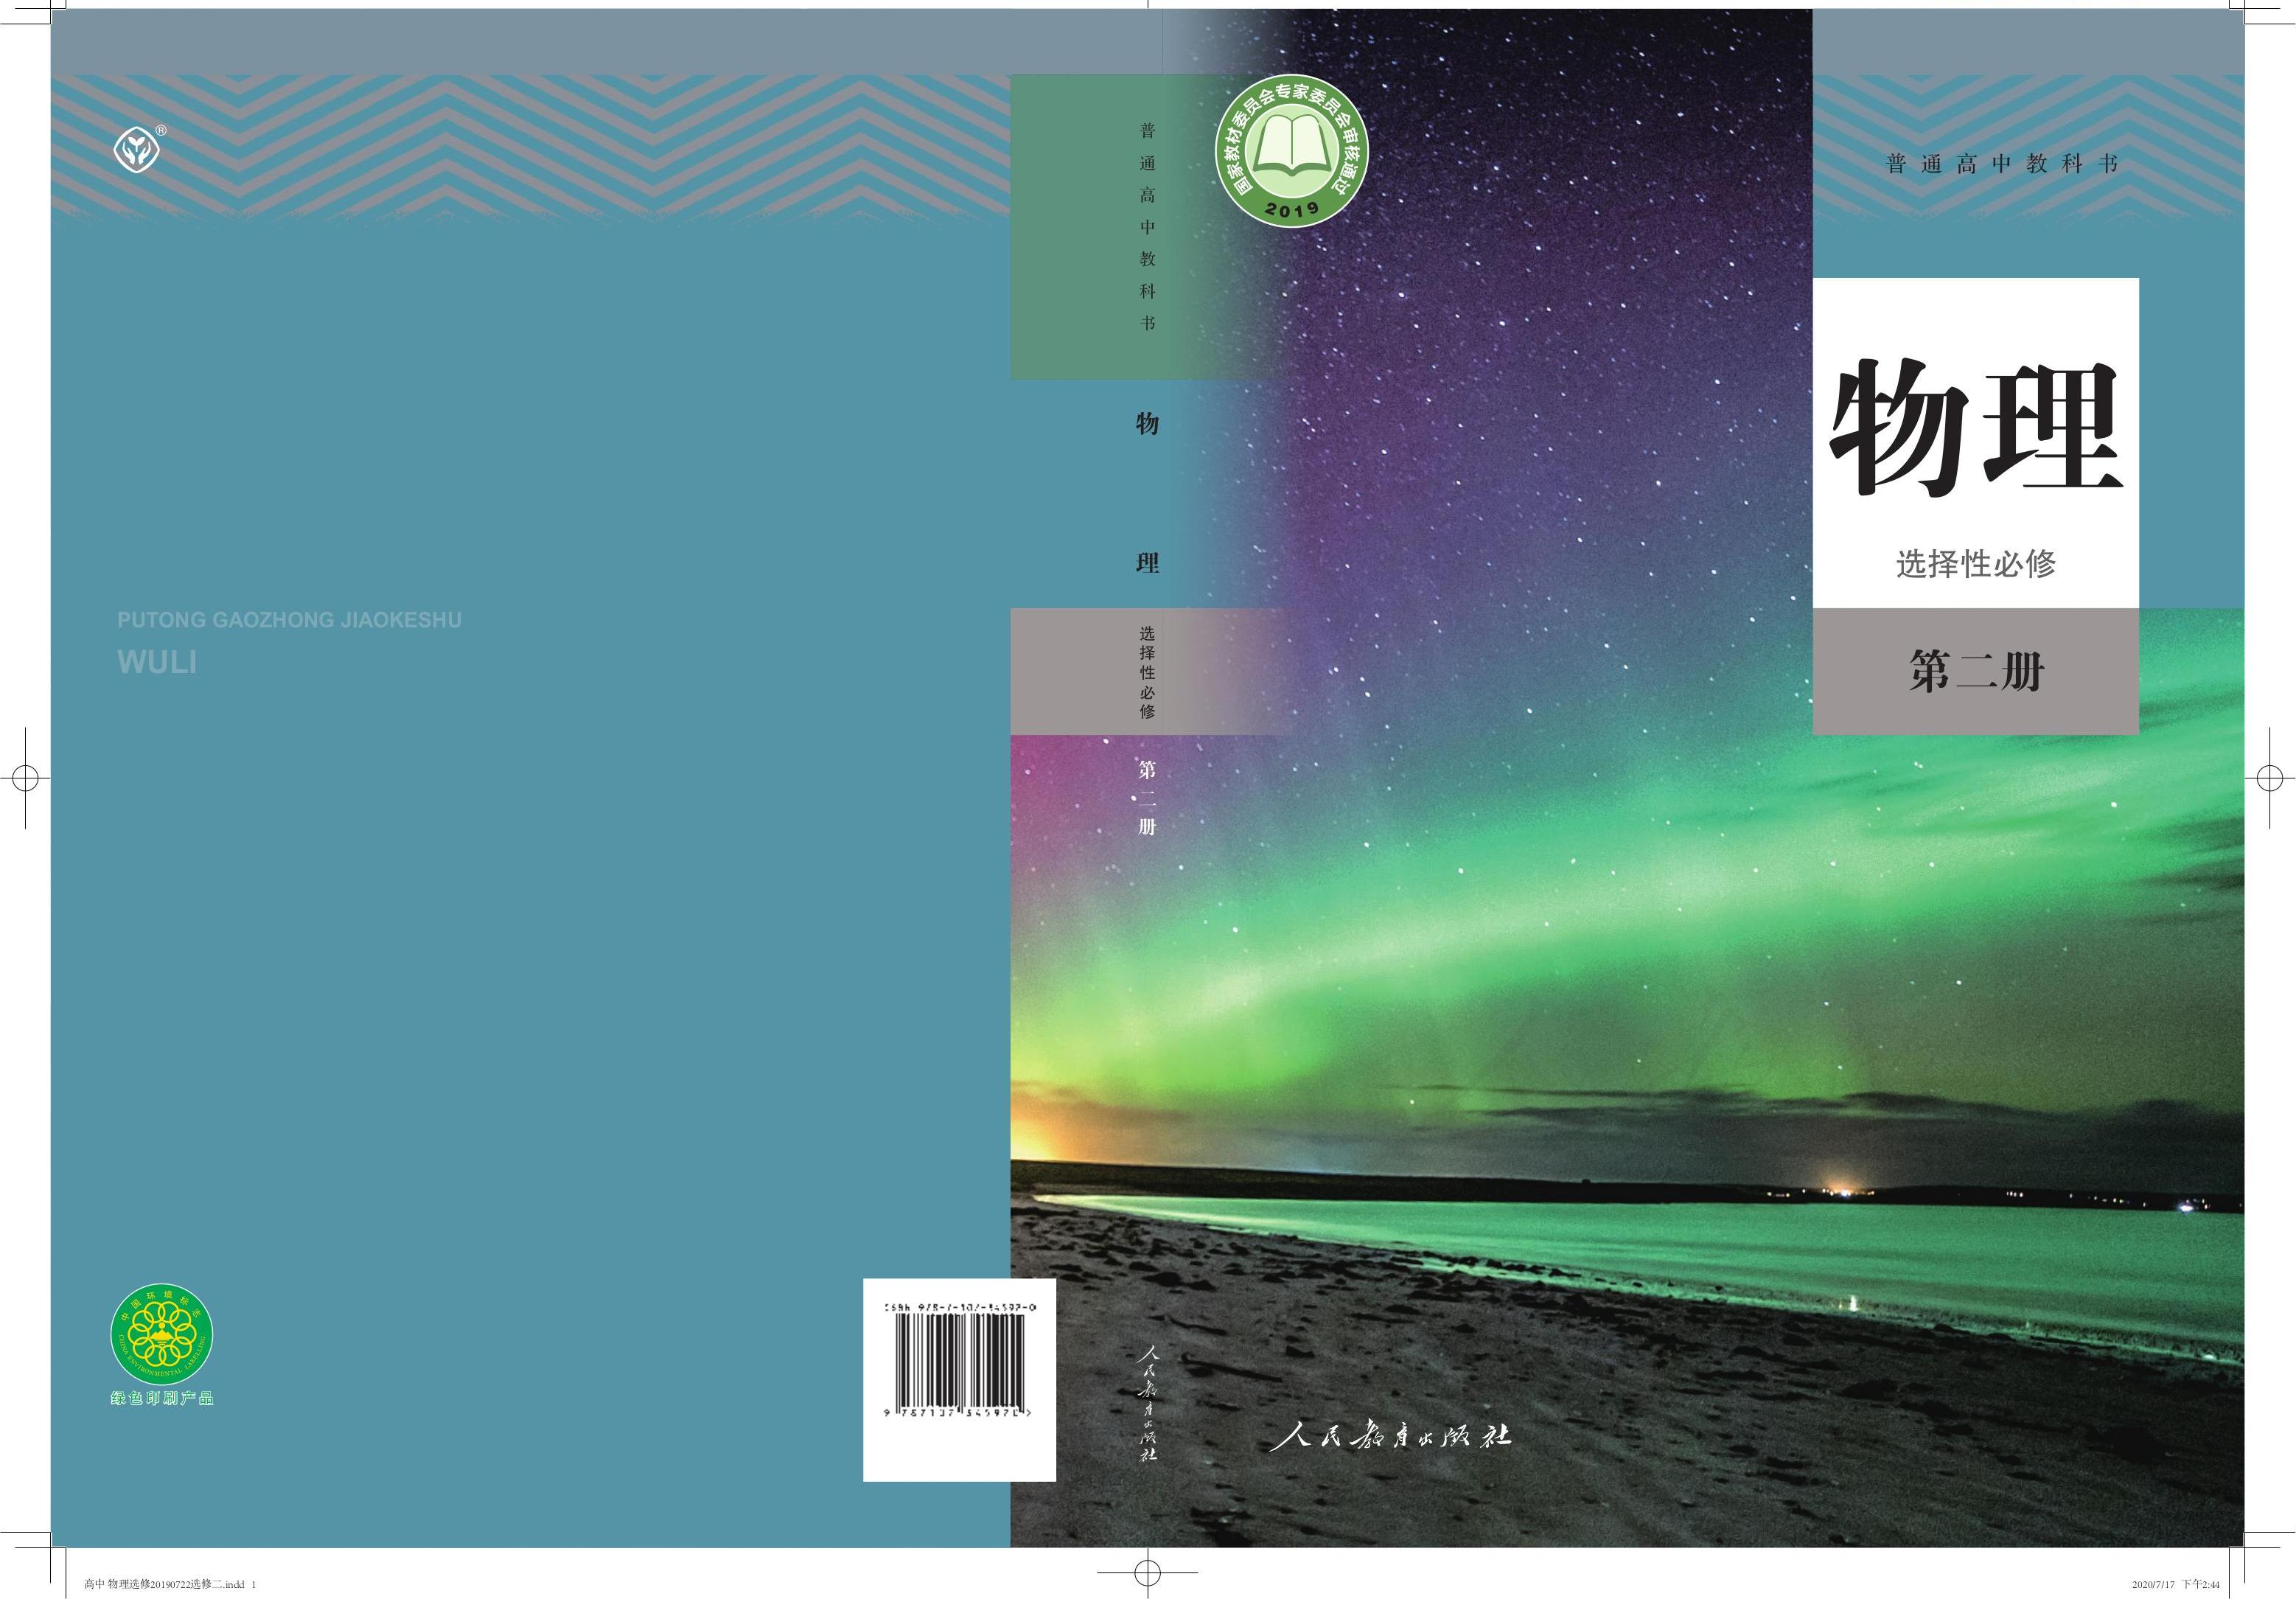
\includegraphics[max width=1.0\textwidth]{images/01910e72-c5b7-7ed5-a6d4-fb3a5faefc32_1_100040.jpg}
\end{center}

普通高中教科书

\section*{物理}

选择性必修

第二册

人民教育出版社 课程教材研究所编著

物理课程教材研究开发中心

人民教育出版社

总 主 编: 彭前程 黄恕伯

本册主编: 谷雅慧 方贵荣

编写人员: (以姓氏笔画为序)

谷雅慧 邹丽晖 金新喜 曹宝龙 彭 征

责任编辑: 付荣兴 苗元秀

美术编辑: 王 艾

普通高中教科书 物理 选择性必修 第二册

人民教育出版社 课程教材研究所

物理课程教材研究开发中心 编著

出版人民众和成社

(北京市海淀区中关村南大街 17 号院 1 号楼 邮编:100081)

网 址 http://www.pep.com.cn

\section*{目 录}

\begin{center}
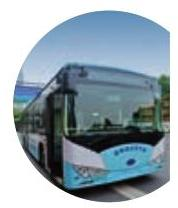
\includegraphics[max width=0.2\textwidth]{images/01910e72-c5b7-7ed5-a6d4-fb3a5faefc32_4_932038.jpg}
\end{center}

1

1. 磁场对通电导线的作用力 2

2. 磁场对运动电荷的作用力 8

3. 带电粒子在匀强磁场中的运动 13

4. 质谱仪与回旋加速器 17

23

1. 楞次定律 24

2. 法拉第电磁感应定律 30

3. 涡流、电磁阻尼和电磁驱动 35

4. 互感和自感 40

48

1. 交变电流 49

2. 交变电流的描述 54

3. 变压器 58

4. 电能的输送 63

70

1. 电磁振荡 71

2. 电磁场与电磁波 76

3. 无线电波的发射和接收 80

4. 电磁波谱 83

90

1. 认识传感器 91

2. 常见传感器的工作原理及应用 97

3. 利用传感器制作简单的自动控制装置 103

课题研究 111

索引 115

\begin{center}
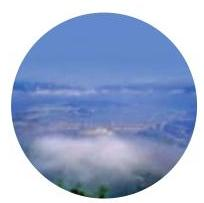
\includegraphics[max width=0.2\textwidth]{images/01910e72-c5b7-7ed5-a6d4-fb3a5faefc32_4_418457.jpg}
\end{center}

\begin{center}
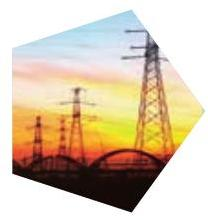
\includegraphics[max width=0.2\textwidth]{images/01910e72-c5b7-7ed5-a6d4-fb3a5faefc32_4_120420.jpg}
\end{center}

\begin{center}
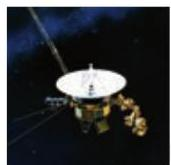
\includegraphics[max width=0.2\textwidth]{images/01910e72-c5b7-7ed5-a6d4-fb3a5faefc32_4_359198.jpg}
\end{center}

\begin{center}
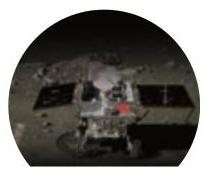
\includegraphics[max width=0.2\textwidth]{images/01910e72-c5b7-7ed5-a6d4-fb3a5faefc32_4_917283.jpg}
\end{center}

\section*{第二章 电磁感应}

\section*{第五章 传感器}

\section*{第四章 电磁振荡与电磁波}

\section*{第一章 安培力与洛伦兹力}

\section*{第三章 交变电流}

\section*{第一章}

安培力与洛伦兹力

奥斯特发现通电导线能使磁针发生偏转, 不仅开启了研究电与磁联系的序幕,还使人们认识了这种神奇的“力”。很快, 人们就在实验中发现了通电导线在磁场中会受到力的作用。电流表、 扬声器、电动机中都有这种作用力。

现在,这种力还能应用到交通工具上,让电动车行驶在街头; 应用到发射台上, 射出数倍音速的炮弹……未来的某一天,可能还会应用到发射塔上,发射航天器……

在这一章里, 就让我们一起去探究这种神奇的作用力吧!

电和磁的实验中最明显的现象是, 处于彼此距离相当远的物体之间的相互作用。因此, 把这些现象化为科学形式的第一步就是, 确定物体之间作用力的大小和方向。

——麦克斯韦

\section*{1 磁场对通电导线的作用力}

\section*{问题}

\begin{center}
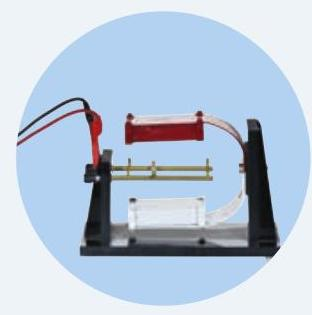
\includegraphics[max width=0.3\textwidth]{images/01910e72-c5b7-7ed5-a6d4-fb3a5faefc32_7_521053.jpg}
\end{center}

在右图中, 当导体棒中有电流流过时, 导体棒就会因受力而发生运动。这个力的方向该如何判断? 它的大小除了与磁感应强度有关外, 还与哪些因素有关?

在必修课中, 我们已经知道了磁场对通电导线有作用力,并从这个现象入手定义了物理量一一磁感应强度 \(B\) 。 安培在研究磁场与电流的相互作用方面作出了杰出的贡献, 为了纪念他, 人们把通电导线在磁场中受的力称为安培力 (Ampère’s force),把电流的单位定为安培 \({}^{\text{①}}\) 。

\begin{center}
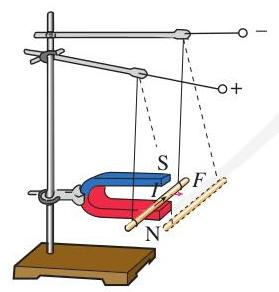
\includegraphics[max width=0.3\textwidth]{images/01910e72-c5b7-7ed5-a6d4-fb3a5faefc32_7_409960.jpg}
\end{center}

图 1.1-1 观察安培力的方向

\section*{安培力的方向}

如图 1.1-1 所示, 把一段导体棒悬挂在蹄形磁体的两极间, 通以电流。研究安培力的方向与哪些因素有关。

\customfootnote{

① 安培也是国际单位制的基本单位之一。真空中相距 \(1\mathrm{\;m}\) 的两根无限长且圆截面可忽略的平行直导线内通过等量恒定电流, 当两导线之间产生的力在每米长度上等于 \(2 \times {10}^{-7}\mathrm{\;N}\) 时,每根导线中通过的电流就是 \(1\mathrm{\;A}\) 。

}

\section*{演示}

\section*{安培力的方向}

按照图 1.1-1 所示, 组装好器材, 进行实验, 观察导体棒受力方向。

1. 上下交换磁极的位置以改变磁场的方向, 观察导体棒受力方向是否改变。

2. 改变导体棒中电流的方向, 观察受力方向是否改变。

实验现象表明, 通电导体棒受力方向与磁场方向、电流方向有关。你能尝试把各种情况下三者的方向画出来, 进行归纳分析, 找到规律吗?

众多事实表明, 通电导线在磁场中所受安培力的方向与电流方向、磁感应强度的方向都垂直 (图 1.1-2)。安培力的方向可用以下方法判定: 伸开左手, 使拇指与其余四个手指垂直,并且都与手掌在同一个平面内;让磁感线从掌心垂直进入,并使四指指向电流的方向,这时拇指所指的方向就是通电导线在磁场中所受安培力的方向 (图 1.1-3 )。这就是判定通电导线在磁场中受力方向的左手定则 ( left-hand rule )。

\begin{center}
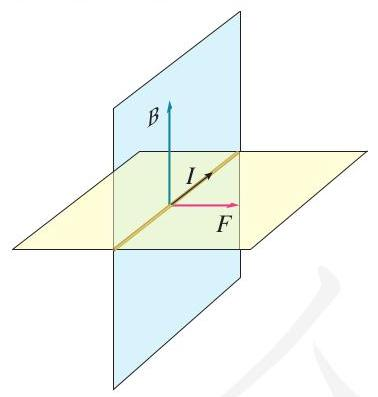
\includegraphics[max width=0.4\textwidth]{images/01910e72-c5b7-7ed5-a6d4-fb3a5faefc32_8_910338.jpg}
\end{center}

图 1.1-2 安培力的方向与电流方

向、磁感应强度的方向都垂直

\begin{center}
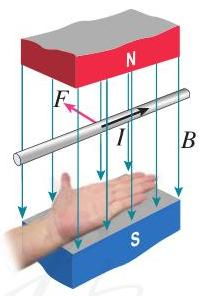
\includegraphics[max width=0.2\textwidth]{images/01910e72-c5b7-7ed5-a6d4-fb3a5faefc32_8_581765.jpg}
\end{center}

图 1.1-3 左手定则

磁场、安培力的问题, 在很多方面都与电场、库仑力的问题相似。然而, 安培力要比库仑力复杂。研究库仑力时, 受力的物体是点电荷, 点电荷受力的方向与电场的方向相同或相反; 但在研究安培力时, 受力的物体是通电导线, 通电导线受力的方向与磁场的方向、电流的方向不但不在一条直线上, 而且不在一个平面里。因此, 研究安培力的问题要涉及三维空间。

\section*{安培力的大小}

在必修课的学习中我们已经知道,垂直于磁场 \(B\) 的方向放置的长为 \(l\) 的一段导线,当通过的电流为 \(I\) 时,它所受的安培力

\[
F = {IlB}
\]

其中力 \(F\) 、电流 \(I\) 、导线长度 \(l\) 、磁感应强度 \(B\) 的单位分别为牛顿 \(\left( \mathrm{N}\right)\) 、安培 \(\left( \mathrm{A}\right)\) 、米 \(\left( \mathrm{m}\right)\) 、特斯拉 \(\left( \mathrm{T}\right)\) 。

当磁感应强度 \(B\) 的方向与通电导线的方向平行时,导线受力为 0 。

\section*{电考与讨论}

当通电导线中的电流方向与磁场方向既不垂直也不平行时, 我们应该如何计算安培力呢?

\begin{center}
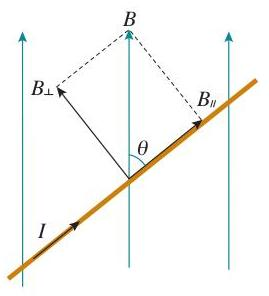
\includegraphics[max width=0.3\textwidth]{images/01910e72-c5b7-7ed5-a6d4-fb3a5faefc32_9_214798.jpg}
\end{center}

图 \({1.1} - {4B}\) 与电流方向的关系

\begin{center}
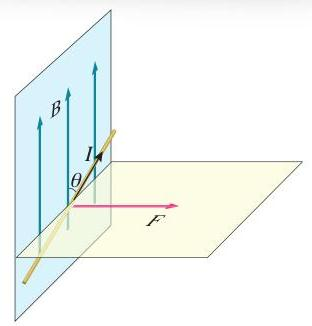
\includegraphics[max width=0.3\textwidth]{images/01910e72-c5b7-7ed5-a6d4-fb3a5faefc32_9_610985.jpg}
\end{center}

图 \({1.1} - {5B}\) 与电流方向夹角为 \(\theta\) 时的受力情况

若磁感应强度 \(B\) 的方向与电流方向成 \(\theta\) 角,根据矢量的运算法则, \(B\) 可以分解为与电流方向垂直的分量 \({B}_{ \bot }\) 和与电流方向平行的分量 \({B}_{//}\) (图 1.1-4)

\[
{B}_{ \bot } = B\sin \theta
\]

\[
{B}_{//} = B\cos \theta
\]

其中 \({B}_{//}\) 对通电导线没有作用力,导线所受的安培力只是 \({B}_{ \bot }\) 产生的。由此得到

\[
F = {IlB}\sin \theta
\]

这就是一般情况下安培力的表达式, \(F\) 的方向如图 1.1-5 所示。

\section*{磁电式电流表}

图 1.1-6 展示了我们实验中常用的磁电式电流表的结构, 它所依据的物理学原理就是通电线圈因受安培力而转动。

\begin{center}
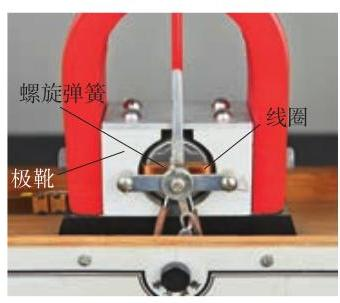
\includegraphics[max width=0.3\textwidth]{images/01910e72-c5b7-7ed5-a6d4-fb3a5faefc32_10_165838.jpg}
\end{center}

图 1.1-6 磁电式电流表的结构

磁电式电流表最基本的组成部分是磁体和放在磁体两极之间的线圈。线圈在磁场中受力的情况如图 1.1-7 所示。 当电流通过线圈时, 导线受到安培力的作用。由左手定则可以判定, 线圈左右两边所受的安培力的方向相反, 于是安装在轴上的线圈就要转动。

\begin{center}
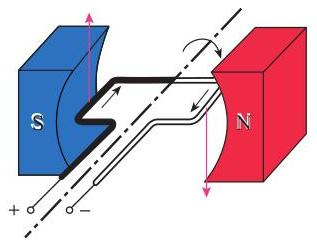
\includegraphics[max width=0.3\textwidth]{images/01910e72-c5b7-7ed5-a6d4-fb3a5faefc32_10_202706.jpg}
\end{center}

图 1.1-7 通电线圈在安培力的作用下发生转动

\begin{center}
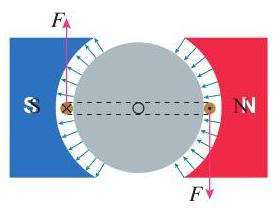
\includegraphics[max width=0.3\textwidth]{images/01910e72-c5b7-7ed5-a6d4-fb3a5faefc32_10_553810.jpg}
\end{center}

图 1.1-8 极靴和铁质圆柱使磁场沿半径方向

线圈转动时, 图 1.1-6 中的螺旋弹簧变形, 以反抗线圈的转动。电流越大, 安培力就越大, 螺旋弹簧的形变也就越大, 线圈偏转的角度也越大, 达到新的平衡。所以, 从线圈偏转的角度就能判断通过电流的大小。

从前面的分析可知, 安培力总与磁感应强度的方向垂直。电流表的两磁极装有极靴, 极靴中间还有一个用软铁制成的圆柱。这样, 极靴与圆柱间的磁场都沿半径方向, 如图 1.1-8 所示。线圈无论转到什么位置, 它的平面都跟磁感线平行, 线圈左右两边所在之处的磁感应强度的大小都相等。

线圈中的电流方向改变时, 安培力的方向随着改变, 指针的偏转方向也随着改变。所以, 根据指针的偏转方向, 可以知道被测电流的方向。

磁电式电流表的优点是灵敏度高, 可以测出很弱的电流; 缺点是线圈的导线很细, 允许通过的电流很弱 (几十微安到几毫安)。如果要用它测量较大的电流, 就要根据在必修第三册中学到的方法扩大其量程。

\section*{科学漫步}

\section*{“电学中的牛顿”——安培}

安培最有影响的科学工作是在电磁学领域。他在得知奥斯特发现电流磁效应的实验后, 第二天就开始实验, 并有了新的发现。安培把导线绕成圆筒状, 制成螺线管。尽管螺线管不是用铁丝而是用铜线绕成的, 但是接通电源以后却能够吸引小铁钉。今天几乎任何电子仪器都离不开线圈, 可见安培这一发现的重要性。

安培做了通电平行导线间相互作用的实验, 证明通电导线间就像磁极和磁极之间一样, 也会发生相互作用。他用不同形状的通电导线进行了许多精巧的实验, 结合严密的数学推演, 得出了关于两条通电导线之间相互作用力的大小和方向的公式。

安培对电磁学的贡献不仅是多方面的, 而且是奠基性的, 麦克斯韦把安培称作 “电学中的牛顿”。安培之所以能够取得重大的研究成就, 是与他的数学修养分不开的。近代科学的重要特点之一是定量分析。数学是科学的语言。系统地应用数学来研究物理学, 是 19 世纪物理学发展的重要特点之一, 这为有数学才能的物理学家创造了用武之地。今天, 数学在科学研究中的作用更为重要。

安培十分重视学术交流。他能敏感地从他人的工作中提出前瞻性的课题, 抓住机遇迅速进入新的研究领域。安培完美的逻辑推理、巧妙的科学实验和精美的数学表达, 令后人赞叹不已。今天, 在各种电器的铭牌上常常可以看到安培名字的第一个字母A,那是人们用电流的单位来纪念安培。

\section*{练习与应用}

1. 图 1.1-9 的磁场中有一条通电导线, 其方向与磁场方向垂直。图 1.1-9 甲、乙、丙分别标明了电流、磁感应强度和安培力三个量中的两个量的方向, 试画出第三个量的方向。(本书用 “: ” 表示磁感线垂直于纸面向外, “ \(\times\) ” 表示磁感线垂直于纸面向里," \(\odot\) ” 表示电流垂直于纸面向外, “ \(\otimes\) ” 表示电流垂直于纸面向里。)

\begin{center}
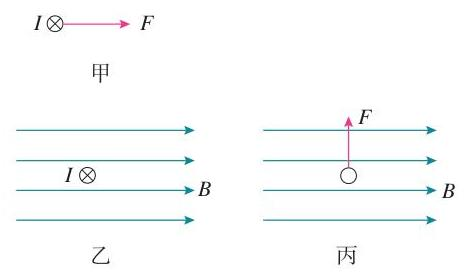
\includegraphics[max width=0.4\textwidth]{images/01910e72-c5b7-7ed5-a6d4-fb3a5faefc32_11_234099.jpg}
\end{center}

图 1.1-9

2. 在图 1.1-10 中画出通电导体棒 \({ab}\) 所受的安培力的方向。

\begin{center}
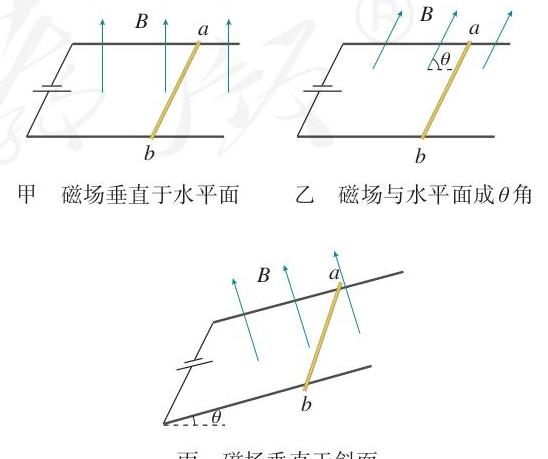
\includegraphics[max width=0.5\textwidth]{images/01910e72-c5b7-7ed5-a6d4-fb3a5faefc32_11_951516.jpg}
\end{center}

图 1.1-10

3. 图 1.1-11 所示为电流天平, 可以用来测量匀强磁场的磁感应强度。它的右臂挂着矩形线圈,匝数为 \(n\) ,线圈的水平边长为 \(l\) ,处于匀强磁场内,磁感应强度 \(B\) 的方向与线圈平面垂直。当线圈中通过电流 \(I\) 时,调节砝码使两臂达到平衡。然后使电流反向, 大小不变。这时需要在左盘中增加质量为 \(m\) 的砝码,才能使两臂再达到新的平衡。

(1) 导出用 \(n\text{、}m\text{、}l\text{、}I\) 表示磁感应强度 \(B\) 的表达式。

( 2 ) 当 \(n = 9,l = {10.0}\mathrm{\;{cm}},I = {0.10}\mathrm{\;A}\) , \(m = {8.78}\mathrm{\;g}\) 时,磁感应强度是多少?

\begin{center}
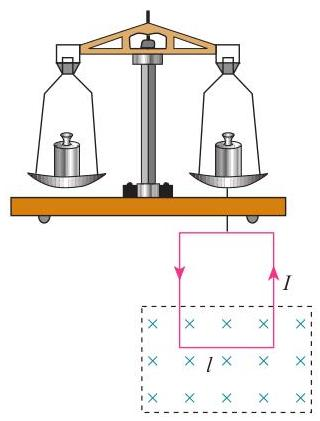
\includegraphics[max width=0.3\textwidth]{images/01910e72-c5b7-7ed5-a6d4-fb3a5faefc32_12_493453.jpg}
\end{center}

图 1.1-11

4. 有人做了一个如图 1.1-12 所示的实验: 把一根柔软的弹簧悬挂起来, 使它的下端刚好跟槽中的水银接触, 观察通电后的现象。请你分析一下, 通电后有可能发生怎样的现象?

\begin{center}
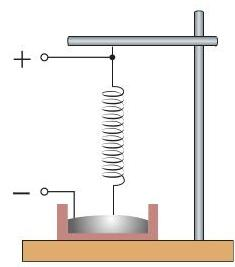
\includegraphics[max width=0.2\textwidth]{images/01910e72-c5b7-7ed5-a6d4-fb3a5faefc32_12_735189.jpg}
\end{center}

图 1.1-12

\section*{2 磁场对运动电荷的作用力}

\section*{问题}

\begin{center}
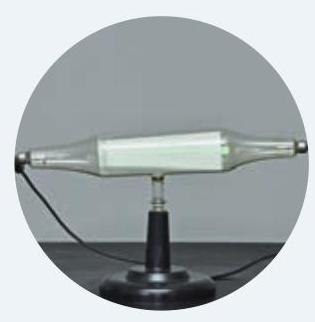
\includegraphics[max width=0.3\textwidth]{images/01910e72-c5b7-7ed5-a6d4-fb3a5faefc32_13_252820.jpg}
\end{center}

我们知道, 磁场对通电导线有作用力; 我们还知道, 带电粒子的定向移动形成了电流。那么, 磁场对运动电荷有作用力吗? 如果有, 力的方向和大小又是怎样的呢?

\section*{洛伦兹力的方向}

\section*{演示}

\section*{观察电子束在磁场中的偏转}

\begin{center}
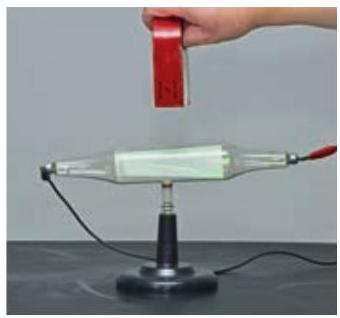
\includegraphics[max width=0.3\textwidth]{images/01910e72-c5b7-7ed5-a6d4-fb3a5faefc32_13_822232.jpg}
\end{center}

图 1.2-1 电子束在磁场中受力偏转

抽成真空的玻璃管左右两个电极分别连接到高压电源两极时, 阴极会发射电子。电子在电场的加速下飞向阳极。 \({}^{\text{①}}\)

没有磁场时, 电子束的径迹呈一条直线。如果在电子束的路径上施加磁场, 电子束会发生弯曲 (图 1.2-1)。改变磁场方向,使其与原来方向相反,电子束会向相反方向弯曲。

\begin{center}
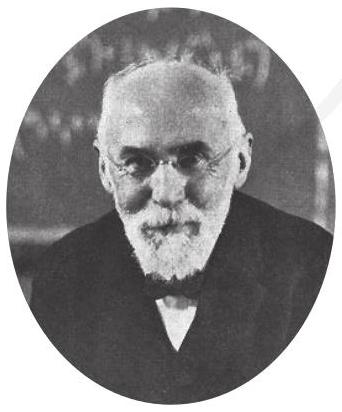
\includegraphics[max width=0.3\textwidth]{images/01910e72-c5b7-7ed5-a6d4-fb3a5faefc32_13_394113.jpg}
\end{center}

洛伦兹(Hendrik Lorentz,1853- 1928 )

实验表明, 电子束受到磁场的力的作用, 径迹发生了弯曲。运动电荷在磁场中受到的力称为洛伦兹力 (Lorentz force )。通电导线在磁场中受到的安培力, 实际是洛伦兹力的宏观表现。运动的带电粒子在磁场中所受洛伦兹力的方向, 与运动方向和磁感应强度的方向都垂直。洛伦兹力的方向可以依照左手定则判定: 伸开左手, 使拇指与其余四个手指垂直,并且都与手掌在同一个平面内;让磁感线从掌心垂直进入,并使四指指向正电荷运动的方向,这时拇

\customfootnote{

① 挡板上有一个扁平的狭缝, 电子飞过挡板后可以形成一个扁平的电子束。长条形的荧光板稍稍倾向轴线, 可以让电子束掠射到荧光板上, 显示出电子束的径迹。

}

指所指的方向就是运动的正电荷在磁场中所受洛伦兹力的方向 (图 1.2-2)。负电荷受力的方向与正电荷受力的方向相反。

\begin{center}
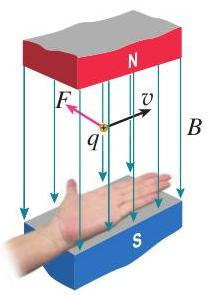
\includegraphics[max width=0.2\textwidth]{images/01910e72-c5b7-7ed5-a6d4-fb3a5faefc32_14_263163.jpg}
\end{center}

图 1.2-2 判断洛伦兹力的方向

\section*{洛伦兹力的大小}

导线中电流的方向与磁场的方向垂直时, 安培力的大小为 \(F = {IlB}\) 。这种情况下,导线中电荷定向运动的方向也与磁场的方向垂直。既然安培力是洛伦兹力的宏观表现, 那么我们是否可以由安培力的表达式推导出洛伦兹力的表达式?

\section*{电考与讨论}

如何由安培力的表达式推导出洛伦兹力的表达式? 建议你沿以下逻辑线索思考。

\begin{center}
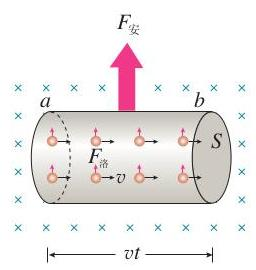
\includegraphics[max width=0.2\textwidth]{images/01910e72-c5b7-7ed5-a6d4-fb3a5faefc32_14_369590.jpg}
\end{center}

图 1.2-3 运动电荷所受洛伦兹力的矢量和在宏观上表现为安培力

1. 设静止导线中定向运动的带电粒子的速度都是 \(v\) ,单位体积内的粒子数为 \({n}_{ \circ }\) 算出图 1.2-3 中一段导线中的粒子数,这就是在时间 \(t\) 内通过横截面 \(S\) 的粒子数。粒子的电荷量记为 \(q\) ,由此可以算出 \(q\) 与电流 \(I\) 的关系。

2. 写出这段长为 \({vt}\) 的导线所受的安培力 \({F}_{\text{安 }}\) 。

3. 求出每个粒子所受的力,它等于洛伦兹力 \({F}_{\text{洛 }}\) 。这时,许多中间量,如 \(n\text{、}S\text{、}t\) 等都应不再出现。

推导时仍然可以认为做定向运动的电荷是正电荷, 所得结果具有普遍性。

电荷量为 \(q\) 的粒子以速度 \(v\) 运动时,如果速度方向与磁感应强度 \(B\) 的方向垂直 (图 1.2-4),那么粒子受到的洛伦兹力为

\[
F = {qvB}
\]

\begin{center}
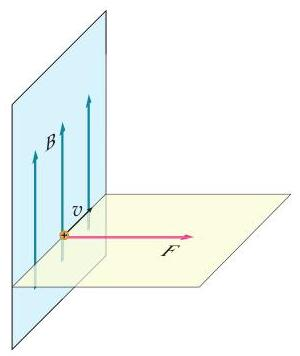
\includegraphics[max width=0.3\textwidth]{images/01910e72-c5b7-7ed5-a6d4-fb3a5faefc32_14_224368.jpg}
\end{center}

图 \({1.2} - {4v}\) 与 \(B\) 垂直

\begin{center}
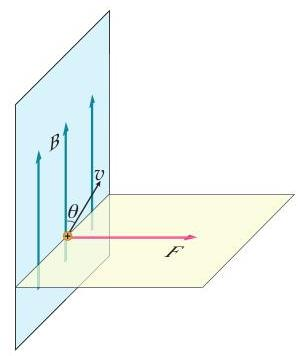
\includegraphics[max width=0.3\textwidth]{images/01910e72-c5b7-7ed5-a6d4-fb3a5faefc32_14_213138.jpg}
\end{center}

图 \({1.2} - {5v}\) 与 \(B\) 不垂直

式中力 \(F\) 、磁感应强度 \(B\) 、电荷量 \(q\) 、速度 \(v\) 的单位分别为牛顿 \(\left( \mathrm{N}\right)\) 、特斯拉 \(\left( \mathrm{T}\right)\) 、库仑 \(\left( \mathrm{C}\right)\) 、米每秒 \(\left( {\mathrm{m}/\mathrm{s}}\right)\) 。

仿照上节对于安培力大小的讨论可以知道, 在一般情况下,当电荷运动的方向与磁场的方向夹角为 \(\theta\) 时 (图 \({1.2} - 5\) ),电荷所受的洛伦兹力为

\[
F = {qvB}\sin \theta
\]

\section*{电子束的磁偏转}

\begin{center}
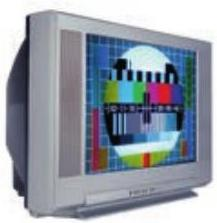
\includegraphics[max width=0.2\textwidth]{images/01910e72-c5b7-7ed5-a6d4-fb3a5faefc32_15_486460.jpg}
\end{center}

图 1.2-6 显像管电视机

洛伦兹力的方向与粒子的运动速度方向垂直, 当粒子在磁场中运动时, 因受到洛伦兹力的作用, 就会发生偏转。显像管电视机 (图 1.2-6) 中就应用了电子束磁偏转的原理。

显像管中有一个电子枪, 工作时它能发射高速电子。 撞击荧光屏, 就能发光。可是, 很细的一束电子打在荧光屏上只能使一个点发光, 要使整个荧光屏发光, 就要靠磁场来使电子束偏转了。

\section*{电考与讨论}

从图 1.2-7 中可以看出, 没有磁场时电子束打在荧光屏正中的 \(O\) 点。为使电子束偏转,由安装在管颈的偏转线圈产生偏转磁场。

\begin{center}
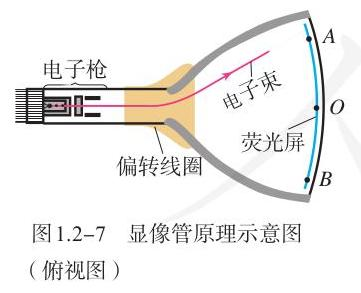
\includegraphics[max width=0.3\textwidth]{images/01910e72-c5b7-7ed5-a6d4-fb3a5faefc32_15_886718.jpg}
\end{center}

1. 要使电子束在水平方向偏离中心, 打在荧光屏上的 \(A\) 点,偏转磁场应该沿什么方向?

2. 要使电子束打在 \(B\) 点,磁场应该沿什么方向?

3. 要使电子束打在荧光屏上的位置由 \(B\) 点逐渐向 \(A\) 点移动, 偏转磁场应该怎样变化?

实际上, 在偏转区的水平方向和竖直方向都有偏转磁场, 其方向、强弱都在不断变化, 因此电子束打在荧光屏上的光点就像图 1.2-8 那样不断移动, 这在显示技术中叫作扫描 (scanning )。电子束从最上一行到最下一行扫描一遍叫作一场, 电视机中的显像管每秒要进行 50 场扫描, 所以我们感到整个荧光屏都在发光。

\begin{center}
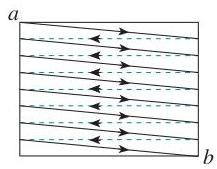
\includegraphics[max width=0.2\textwidth]{images/01910e72-c5b7-7ed5-a6d4-fb3a5faefc32_16_708703.jpg}
\end{center}

图 1.2-8 电子束在荧光屏上扫描

\section*{科学漫步}

\section*{正电子的发现}

在粒子物理研究中, 带电粒子在云室等探测装置中的径迹是非常重要的实验证据。根据对不同粒子径迹的分析和比较, 科学家可以得到粒子的带电情况、 运动情况等许多信息, 甚至可以发现新粒子。

\begin{center}
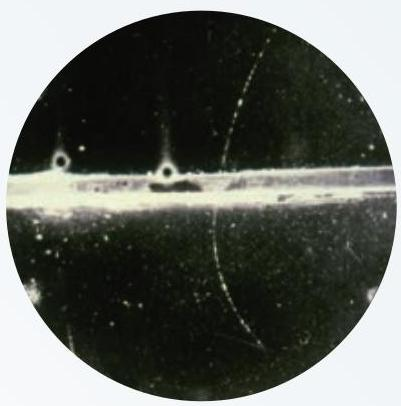
\includegraphics[max width=0.4\textwidth]{images/01910e72-c5b7-7ed5-a6d4-fb3a5faefc32_16_482571.jpg}
\end{center}

图 1.2-9 安德森记录的正电子的径迹

1930 年, 英国物理学家狄拉克从理论上预言了电子的反粒子的存在, 这个反粒子就是正电子。正电子与电子质量相同, 但是带等量的正电荷, 也可以说, 它是带正电荷的电子。

1932 年, 美国物理学家安德森在宇宙线实验中发现了正电子。他利用放在强磁场中的云室来记录宇宙线粒子,并在云室中加入一块厚 \(6\mathrm{\;{mm}}\) 的铅板,借以减慢粒子的速度。当宇宙线粒子通过云室内的强磁场时, 拍下粒子径迹的照片, 如图 1.2-9所示。

由于所加铅板降低了粒子的运动速度, 粒子在磁场中偏转的轨道半径就会变小, 所以根据铅板上下粒子径迹的偏转情况,可以判定粒子的运动方向 (图 1.2-9 中的粒子是由上向下运动的 )。 这个粒子的径迹与电子的径迹十分相似, 只是偏转方向相反。由此, 安德森发现了正电子, 并由于这一发现, 获得了 1936 年的诺贝尔物理学奖。

在安德森这一发现之前不久, 约里奥-居里夫妇也在云室照片中发现了与电子偏转方向相反的粒子径迹。如果他们意识到这个粒子所带电荷与电子相反, 就会把研究工作引向正电子的发现。但遗憾的是, 他们没有认真研究这一现象, 只是提出了一个经不住推敲的解释, 就把这一特殊现象放走了。他们认为, 这是向放射源移动的电子的径迹, 而不是从放射源发出的正电子的径迹。他们没有思考, 向放射源移动的电子来自何处, 也没有设法判断这个粒子的运动方向。得知安德森的发现后, 约里奥-居里夫妇证实, 他们使用的钋加铍源发射的射线能够产生正负电子对。 他们后来也记录到了单个正电子的径迹。

正电子的发现证明了反物质的存在, 对反物质世界的探索现在仍是物理学的前沿之一。

\section*{(练习与应用}

1. 电子的速率 \(v = {3.0} \times {10}^{6}\mathrm{\;m}/\mathrm{s}\) ,沿着与磁场垂直的方向射入 \(B = {0.10}\mathrm{\;T}\) 的匀强磁场中, 它受到的洛伦兹力多大?

2. 试判断图 1.2-10 所示的带电粒子刚进入磁场时所受到的洛伦兹力的方向。

\begin{center}
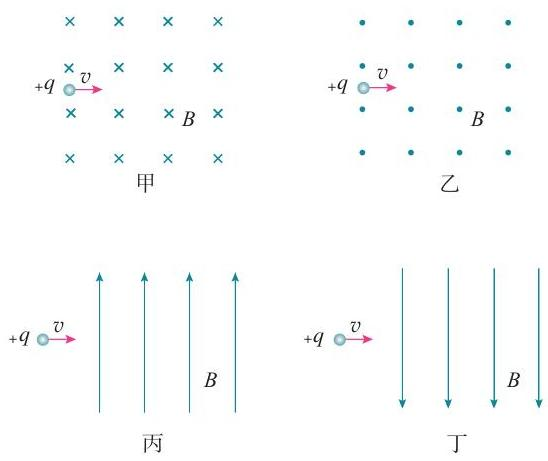
\includegraphics[max width=0.5\textwidth]{images/01910e72-c5b7-7ed5-a6d4-fb3a5faefc32_17_368660.jpg}
\end{center}

图 1.2-10

3. 在图 1.2-11 所示的平行板器件中, 电场强度 \(E\) 和磁感应强度 \(B\) 相互垂直。具有不同水平速度的带电粒子射入后发生偏转的情况不同。 这种装置能把具有某一特定速度的粒子选择出来, 所以叫作速度选择器。试证明带电粒子具有速度 \(v = \frac{E}{B}\) 时,才能沿着图示虚线路径通过这个速度选择器。

\begin{center}
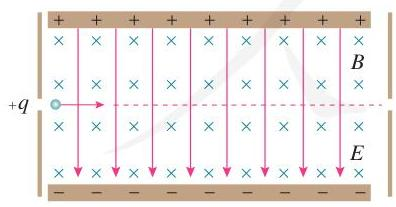
\includegraphics[max width=0.4\textwidth]{images/01910e72-c5b7-7ed5-a6d4-fb3a5faefc32_17_945085.jpg}
\end{center}

图 1.2-11

4. 一种用磁流体发电的装置如图 1.2-12 所示。平行金属板 A、B 之间有一个很强的磁场, 将一束等离子体 (即高温下电离的气体, 含有大量正、负带电粒子)喷入磁场, A、B两板间便产生电压。如果把 A、B 和用电器连接, A、 \(\mathrm{B}\) 就是一个直流电源的两个电极。

(1) A、B板哪一个是电源的正极?

(2)若A、B两板相距为 \(d\) ,板间的磁场按匀强磁场处理,磁感应强度为 \(B\) ,等离子体以速度 \(v\) 沿垂直于 \(B\) 的方向射入磁场,这个发电机的电动势是多大?

\begin{center}
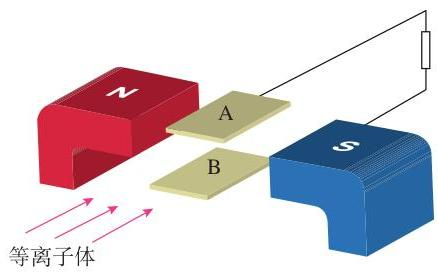
\includegraphics[max width=0.4\textwidth]{images/01910e72-c5b7-7ed5-a6d4-fb3a5faefc32_17_644790.jpg}
\end{center}

图 1.2-12

5. 我们已经知道, 垂直于匀强磁场磁感线的通电导线所受的安培力 \(F = {IlB}\) ,由此,我们用 \(B = \frac{F}{Il}\) 来定义磁感应强度。同样,运动方向垂直于匀强磁场磁感线的带电粒子所受的洛伦兹力 \(F = {qvB}\) ,由此也可以用洛伦兹力来定义磁感应强度, 这样得到磁感应强度的定义式是怎样的? 把这个定义式与电场强度的定义式 \(E = \frac{F}{q}\) 进行对比,这两个定义式的差别在哪里? 通过对这两个定义式的对比, 你能获得哪些认识?

\section*{3 带电粒子在匀强磁场中的运动}

\section*{问题}

\begin{center}
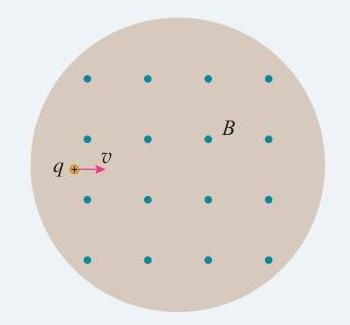
\includegraphics[max width=0.3\textwidth]{images/01910e72-c5b7-7ed5-a6d4-fb3a5faefc32_18_600709.jpg}
\end{center}

在现代科学技术中, 常常要研究带电粒子在磁场中的运动。如果沿着与磁场垂直的方向发射一束带电粒子, 请猜想这束粒子在匀强磁场中的运动径迹, 你猜想的依据是什么?

\section*{带电粒子在匀强磁场中的运动}

要分析上述问题中带电粒子的运动, 就需要分析粒子的受力情况。我们知道, 带电粒子在磁场中运动要受到洛伦兹力的作用。由于带电粒子初速度的方向和洛伦兹力的方向都在与磁场方向垂直的平面内, 所以粒子在这个平面内运动。

\begin{center}
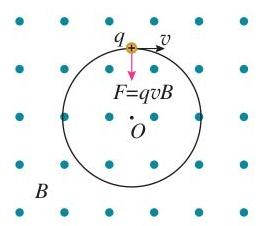
\includegraphics[max width=0.2\textwidth]{images/01910e72-c5b7-7ed5-a6d4-fb3a5faefc32_18_493803.jpg}
\end{center}

图 1.3-1 带电粒子在匀强磁场中做匀速圆周运动

洛伦兹力总是与粒子的运动方向垂直, 只改变粒子速度的方向, 不改变粒子速度的大小。由于粒子速度的大小不变, 粒子在匀强磁场中所受洛伦兹力的大小也不改变, 洛伦兹力对粒子起到了向心力的作用。所以, 沿着与磁场垂直的方向射入磁场的带电粒子, 在匀强磁场中做匀速圆周运动 (图 1.3-1 )。

\section*{电考与讨论}

垂直射入磁场的带电粒子在匀强磁场中做匀速圆周运动, 圆周的半径可能与哪些因素有关? 周期可能与哪些因素有关?

\section*{带电粒子在磁场中做圆周运动的半径和周期}

考虑到粒子所受的洛伦兹力提供了它做匀速圆周运动的向心力, 列出方程来就不难得到几个物理量之间的关系式。然后就可以分别判断粒子的速度和磁场的强弱对圆半径的影响。

假设一个电荷量为 \(q\) 的粒子,在磁感应强度为 \(B\) 的匀强磁场中以速度 \(v\) 运动,那么带电粒子所受的洛伦兹力为

\[
F = {qvB}
\]

洛伦兹力提供向心力

\[
{qvB} = m\frac{{v}^{2}}{r}
\]

由此可解得圆周运动的半径

\[
r = \frac{mv}{qB}
\]

从这个结果可以看出, 粒子在匀强磁场中做匀速圆周运动的半径与它的质量、速度成正比, 与电荷量、磁感应强度成反比。

\section*{演 示}

\section*{观察带电粒子的运动径迹}

图 1.3-2 是洛伦兹力演示仪的示意图。电子枪可以发射电子束。玻璃泡内充有稀薄的气体, 在电子束通过时能够显示电子的径迹。励磁线圈能够在两个线圈之间产生匀强磁场, 磁场的方向与两个线圈中心的连线平行。

分别预测下列情况下带电粒子的运动径迹, 然后用洛伦兹力演示仪进行检验。

\begin{center}
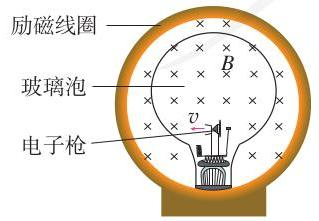
\includegraphics[max width=0.3\textwidth]{images/01910e72-c5b7-7ed5-a6d4-fb3a5faefc32_19_635305.jpg}
\end{center}

图 1.3-2 洛伦兹力演示仪示意图

1. 不加磁场。

2. 在玻璃泡中施加沿两线圈中心连线方向、由读者指向纸面的磁场。

3. 保持出射电子的速度不变, 改变磁感应强度。

4. 保持磁感应强度不变, 改变出射电子速度的大小和方向。

在前面的实验中, 不加磁场时, 电子束的径迹是一条直线 (图 1.3-3)。加磁场后电子束的径迹是一个圆 (图 1.3-4)。当电子束出射速度不变, 磁感应强度变大时, 这个圆的半径变小; 当磁感应强度不变, 电子束出射速度变大时, 这个圆的半径变大。

\begin{center}
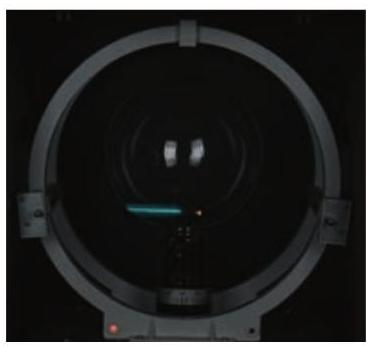
\includegraphics[max width=0.3\textwidth]{images/01910e72-c5b7-7ed5-a6d4-fb3a5faefc32_20_973485.jpg}
\end{center}

图 1.3-3 没有磁场时电子束沿直线运动

我们还可以根据圆周运动的知识分析带电粒子做匀速圆周运动的周期。匀速圆周运动的周期 \(T = \frac{2\pi r}{v}\) ,将 \(r = \frac{mv}{qB}\) 代入,可得

\[
T = \frac{2\pi m}{qB}
\]

\begin{center}
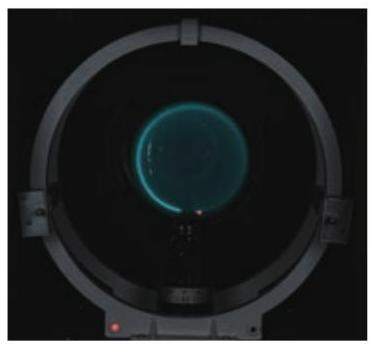
\includegraphics[max width=0.4\textwidth]{images/01910e72-c5b7-7ed5-a6d4-fb3a5faefc32_20_512596.jpg}
\end{center}

图 1.3-4 施加垂直于纸面的磁场后, 电子束沿圆轨道运动

由此可见, 带电粒子在匀强磁场中做匀速圆周运动的周期跟轨道半径和运动速度无关。这是一个很重要的结论, 下一节介绍的回旋加速器就是依据这个原理制成的。

\section*{【例题】}

一个质量为 \({1.67} \times {10}^{-{27}}\mathrm{\;{kg}}\) 、电荷量为 \({1.6} \times {10}^{-{19}}\mathrm{C}\) 的带电粒子,以 \(5 \times {10}^{5}\mathrm{\;m}/\mathrm{s}\) 的初速度沿与磁场垂直的方向射入磁感应强度为 \({0.2}\mathrm{\;T}\) 的匀强磁场。

(1)求粒子所受的重力和洛伦兹力的大小之比。

(2)求粒子在磁场中运动的轨道半径。

(3)求粒子做匀速圆周运动的周期。

分析 依据所给数据分别计算出带电粒子所受的重力和洛伦兹力, 就可求出所受重力与洛伦兹力之比。带电粒子在匀强磁场中受洛伦兹力并做匀速圆周运动, 由此可以求出粒子运动的轨道半径及周期。

解 ( 1 ) 粒子所受的重力

\[
G = {mg} = {1.67} \times {10}^{-{27}} \times {9.8}\mathrm{\;N} = {1.64} \times {10}^{-{26}}\mathrm{\;N}
\]

所受的洛伦兹力

\[
F = {qvB} = {1.6} \times {10}^{-{19}} \times 5 \times {10}^{5} \times {0.2}\mathrm{\;N} = {1.6} \times {10}^{-{14}}\mathrm{\;N}
\]

重力与洛伦兹力之比

\[
\frac{G}{F} = \frac{{1.64} \times {10}^{-{26}}}{{1.6} \times {10}^{-{14}}} = {1.03} \times {10}^{-{12}}
\]

可见, 带电粒子在磁场中运动时, 洛伦兹力远大于重力, 重力作用的影响可以忽略。

(2)带电粒子所受的洛伦兹力为

\[
F = {qvB}
\]

洛伦兹力提供向心力, 故

\[
{qvB} = m\frac{{v}^{2}}{r}
\]

由此得到粒子在磁场中运动的轨道半径

\[
r = \frac{mv}{qB} = \frac{{1.67} \times {10}^{-{27}} \times 5 \times {10}^{5}}{{1.6} \times {10}^{-{19}} \times {0.2}}\mathrm{\;m} = {2.61} \times {10}^{-2}\mathrm{\;m}
\]

(3)粒子做匀速圆周运动的周期

\[
T = \frac{2\pi r}{v} = \frac{2\pi m}{qB} = \frac{2 \times {3.14} \times {1.67} \times {10}^{-{27}}}{{1.6} \times {10}^{-{19}} \times {0.2}}\mathrm{\;s} = {3.28} \times {10}^{-7}\mathrm{\;s}
\]

\section*{练习与应用}

1. 电子以 \({1.6} \times {10}^{6}\mathrm{\;m}/\mathrm{s}\) 的速度沿着与磁场垂直的方向射入 \(B = {2.0} \times {10}^{-4}\mathrm{\;T}\) 的匀强磁场中。 求电子做匀速圆周运动的轨道半径和周期。

2. 已知氚核的质量约为质子质量的 3 倍, 带正电荷,电荷量为一个元电荷; \(\alpha\) 粒子即氦原子核, 质量约为质子质量的 4 倍, 带正电荷, 电荷量为 \(e\) 的 2 倍。现在质子、氚核和 \(\alpha\) 粒子在同一匀强磁场中做匀速圆周运动。求下列情况中它们运动的半径之比:

(1)它们的速度大小相等。

(2)它们由静止经过相同的加速电场加速后进入磁场。

3. 如图 1.3-5 所示,一个质量为 \(m\) 、电荷量为 \(q\) 的带负电荷的粒子,不计重力,从 \(x\) 轴上的 \(P\) 点以速度 \(v\) 射入第一象限内的匀强磁场中,并恰好垂直于 \(y\) 轴射出第一象限。已知 \(v\) 与 \(x\) 轴成 \({60}^{ \circ }\) 角, \({OP} = a\) 。

(1)求匀强磁场的磁感应强度 \(B\) 的大小。

(2)求带电粒子穿过第一象限所用的时间。

\begin{center}
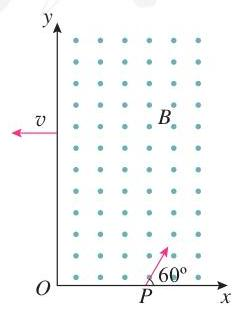
\includegraphics[max width=0.2\textwidth]{images/01910e72-c5b7-7ed5-a6d4-fb3a5faefc32_21_337275.jpg}
\end{center}

图 1.3-5

\section*{4 质谱仪与回旋加速器}

\section*{问题}

\begin{center}
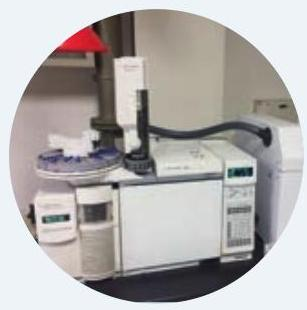
\includegraphics[max width=0.3\textwidth]{images/01910e72-c5b7-7ed5-a6d4-fb3a5faefc32_22_732216.jpg}
\end{center}

在科学研究和工业生产中, 常需要将一束带等量电荷的粒子分开, 以便知道其中所含物质的成分。利用所学的知识, 你能设计一个方案, 以便分开电荷量相同、质量不同的带电粒子吗?

\section*{质谱仪}

我们知道, 电场可以对带电粒子施加作用力, 磁场也可以对运动的带电粒子施加作用力。可以利用电场和磁场来控制带电粒子的运动。利用电场让带电粒子获得一定的速度,利用磁场让粒子做圆周运动。由 \(r = \frac{mv}{qB}\) 可知,带电粒子在匀强磁场中做匀速圆周运动的半径与质量有关, 如果 \(B\text{、}v\) 相同, \(m\) 不同,则 \(r\) 不同,这样就可以把不同的粒子分开。

19 世纪末, 汤姆孙的学生阿斯顿就按照这样的想法设计了质谱仪, 并用质谱仪发现了氖 -20 和氖 -22, 证实了同位素的存在。后来经过多次改进, 质谱仪已经成为一种十分精密的仪器, 是科学研究和工业生产中的重要工具。

\begin{center}
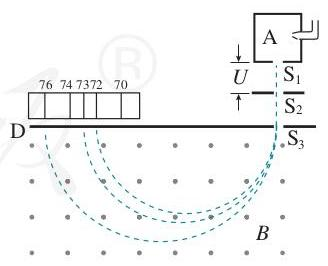
\includegraphics[max width=0.3\textwidth]{images/01910e72-c5b7-7ed5-a6d4-fb3a5faefc32_22_634528.jpg}
\end{center}

图 1.4-1 质谱仪工作原理

如图 1.4-1 所示,质量为 \(m\) 、电荷量为 \(q\) 的粒子,从容器 \(\mathrm{A}\) 下方的小孔 \({\mathrm{S}}_{1}\) 飘入电势差为 \(U\) 的加速电场,其初速度几乎为 0,然后经过 \({\mathrm{S}}_{3}\) 沿着与磁场垂直的方向进入磁感应强度为 \(B\) 的匀强磁场中,最后打到照相底片 \(\mathrm{D}\) 上。

粒子进入磁场时的速度 \(v\) 等于它在电场中被加速而得到的速度。由动能定理得

\[
\frac{1}{2}m{v}^{2} = {qU}
\]

由此可知

\[
v = \sqrt{\frac{2qU}{m}} \tag{1}
\]

粒子在磁场中只受洛伦兹力的作用, 做匀速圆周运动, 圆周的半径为

\[
r = \frac{mv}{qB} \tag{(2)}
\]

把 (1) 式中的 \(v\) 代入 (2) 式,得出粒子在磁场中做匀速圆周运动的轨道半径

\[
r = \frac{1}{B}\sqrt{\frac{2mU}{q}}
\]

如果容器 \(\mathrm{A}\) 中粒子的电荷量相同而质量不同,它们进入匀强磁场后将沿着不同的半径做圆周运动, 因而被分开, 并打到照相底片的不同地方。

实际工作中, 往往让中性的气体分子进入电离室 A, 在那里被电离成离子, 这些离子从电离室的小孔 “飘” 出, 从缝 \({\mathrm{S}}_{1}\) 进入加速电场中被加速。然后让离子垂直进入匀强磁场中做匀速圆周运动, 最后打在照相底片 \(\mathrm{D}\) 上。从离子打在底片上的位置可以测出圆周的半径 \(r\) ,进而可以算出离子的比荷 \(\frac{q}{m}\) 。

\section*{回旋加速器}

要认识原子核内部的情况, 必须把核 “打开” 进行 “观察”。然而, 原子核被强大的核力约束, 只有用极高能量的粒子作为 “炮弹” 去轰击, 才能把它 “打开”。产生这些高能 “炮弹” 的 “工厂” 就是各种各样的粒子加速器。

由于库仑力可以对带电粒子做功, 从而增加粒子的动能, 因此, 人们首先想到加速器中一定要用到电场。加速电压越高, 粒子获得的动能就越高。然而产生过高的电压在技术上是很困难的, 于是人们就会进一步设想, 能不能采用多次 (多级) 加速的方法呢?

在图 1.4-2 所示的多级加速器中, 各加速区的两板之间用独立电源供电,所以粒子从 \({\mathrm{P}}_{2}\) 飞向 \({\mathrm{P}}_{3}\text{、}\) 从 \({\mathrm{P}}_{4}\) 飞向 \({\mathrm{P}}_{5}\cdots \cdots\) 时不会减速。由于粒子在加速过程中的径迹为直线, 要得到较高动能的粒子, 其加速装置要很长。人们进一步思考, 如果带电粒子在一次加速后又转回来被第二次加速, 如此往复 “转圈圈” 式地被加速, 加速器装置所占的空间不是会大大缩小吗? 而磁场正好能使带电粒子 “转圈圈”! 于是, 人们依据这个思路设计出了用磁场控制轨道、用电场进行加速的回旋加速器 (cyclotron)。

\begin{center}
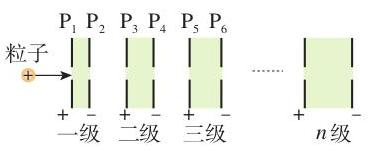
\includegraphics[max width=0.4\textwidth]{images/01910e72-c5b7-7ed5-a6d4-fb3a5faefc32_24_218887.jpg}
\end{center}

图 1.4-2 多级加速器

回旋加速器的工作原理如图 1.4-3 所示。 \({\mathrm{D}}_{1}\) 和 \({\mathrm{D}}_{2}\) 是两个中空的半圆金属盒,它们之间有一定的电势差 \(U\) 。 \(A\) 处的粒子源产生的带电粒子, 在两盒之间被电场加速。两个半圆盒处于与盒面垂直的匀强磁场中, 所以粒子在磁场中做匀速圆周运动。经过半个圆周之后, 当粒子再次到达两盒间的缝隙时, 这时控制两盒间的电势差, 使其恰好改变正负, 于是粒子经过盒缝时再一次被加速。如此, 粒子在做圆周运动的过程中一次一次地经过盒缝, 而两盒间的电势差一次一次地改变正负, 粒子的速度就能够增加到很大。

\begin{center}
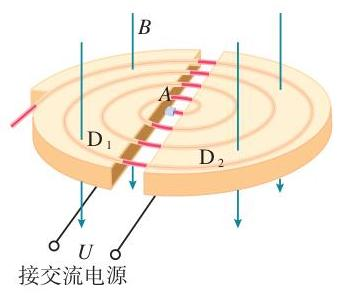
\includegraphics[max width=0.3\textwidth]{images/01910e72-c5b7-7ed5-a6d4-fb3a5faefc32_24_182927.jpg}
\end{center}

图 1.4-3 回旋加速器的原理

\section*{思考与讨论}

假如粒子每两次经过盒缝的时间间隔 \({}^{\mathbb{O}}\) 相同,控制两盒间电势差的正负变换是比较容易的。但是粒子的运动越来越快, 也许粒子走过半圆的时间间隔越来越短, 这样两盒间电势差的正负变换就要越来越快, 从而造成技术上的一个难题。实际情况是这样吗?

带电粒子在匀强磁场中做匀速圆周运动的周期 \(T = \frac{2\pi m}{qB}\) 。对一定的带电粒子和一定的磁场来说,这个周期是不变的, 尽管粒子的速率和半径一次比一次大, 运动周期却始终不变。这样, 如果在两盒间加一个交变电场, 使它也以同样的周期往复变化, 那就可以保证粒子每经过电场时, 都正好赶上适合的电场方向而被加速。

\customfootnote{

① 指粒子经过半圆轨道所用的时间。盒缝宽度远小于盒半径 (图 1.4-3 夸大了缝的宽度), 粒子通过盒缝的时间可以忽略。

}

回旋加速器加速的带电粒子,能量达到 \({25} \sim {30}\mathrm{{MeV}}\) 后, 很难再加速了。原因是, 按照狭义相对论, 粒子的质量随着速度增加而增大, 而质量的变化会导致其回转周期的变化, 从而破坏了与电场变化周期的同步。

\section*{练习与应用}

1. A、B 是两种同位素的原子核, 它们具有相同的电荷、不同的质量。为测定它们的质量比, 使它们从质谱仪的同一加速电场由静止开始加速, 然后沿着与磁场垂直的方向进入同一匀强磁场, 打到照相底片上。如果从底片上获知 \(\mathrm{A}\text{、}\mathrm{\;B}\) 在磁场中运动轨迹的直径之比是 \({1.08} : 1\) ,求 \(\mathrm{A}\text{、}\mathrm{\;B}\) 的质量之比。

2. 回旋加速器 \(\mathrm{D}\) 形盒的半径为 \(r\) ,匀强磁场的磁感应强度为 \({B}_{ \circ }\) 一个质量为 \({m}_{ \smallsetminus }\) 电荷量为 \(q\) 的粒子在加速器的中央从速度为 0 开始加速。 根据回旋加速器的这些数据, 估算该粒子离开回旋加速器时获得的动能。

3. 如图 1.4-4 所示, 一束电子以垂直于磁感应强度 \(B\) 并垂直于磁场边界的速度 \(v\) 射入宽度为 \(d\) 的匀强磁场中,穿出磁场时速度方向和原来射入方向的夹角为 \(\theta = {60}^{ \circ }\) ,求电子的比荷和穿越磁场的时间。

4. 回旋加速器两个 \(\mathrm{D}\) 形金属盒分别和一高频交流电源两极相接, 两盒放在磁感应强度为 \(B\) 的匀强磁场中,磁场方向垂直于盒底面, 粒子源置于盒的圆心附近。若粒子源射出的粒子电荷量为 \(q\) ,质量为 \(m\) ,粒子最大回旋半径为 \(R\) 。

(1)粒子在盒内做何种运动?

(2)求所加交流电源的频率。

(3)求粒子加速后获得的最大动能。

\begin{center}
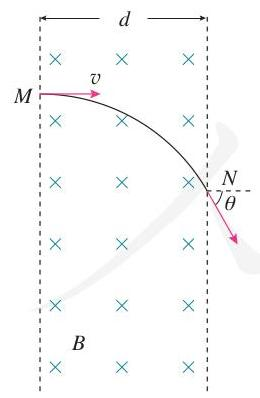
\includegraphics[max width=0.2\textwidth]{images/01910e72-c5b7-7ed5-a6d4-fb3a5faefc32_25_896161.jpg}
\end{center}

图 1.4-4

A 组

1. 有人说: “通电导线放在磁感应强度为 0 的位置上, 所受的安培力一定为 0 , 因此, 当某位置的通电导线不受安培力时, 该位置的磁感应强度一定为 0 。” 你认为他说的话对吗? 为什么?

2. 把一根通电的硬导线放在磁场中, 导线所在区域的磁感线呈弧形, 如图 1-1 所示。导线可以在空中自由移动和转动, 导线中的电流方向由 \(a\) 向 \(b\) 。

(1)描述导线的运动情况。

(2)虚线框内有产生以上弧形磁感线的磁场源, 它可能是条形磁体、蹄形磁体、通电螺线管、直线电流。请你分别按每种可能考虑, 大致画出它们的安放位置。

\begin{center}
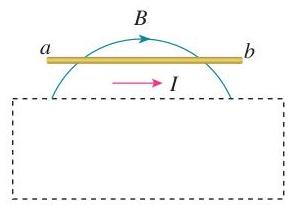
\includegraphics[max width=0.3\textwidth]{images/01910e72-c5b7-7ed5-a6d4-fb3a5faefc32_26_346378.jpg}
\end{center}

图 1-1

3. 如图 1-2 所示, 把轻质导线圈用绝缘细线悬挂在磁体 \(\mathrm{N}\) 极附近,磁体的轴线穿过线圈的圆心且垂直线圈平面。当线圈内通以图示方向的电流后, 线圈的运动情况怎样? 请用以下两种方法分析:

(1)把整个线圈看成一个通电螺线管。

(2)把线圈截成许多小段, 每小段视为通电直导线, 分析磁场对各小段导线的作用力。

\begin{center}
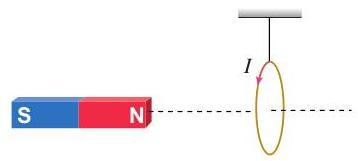
\includegraphics[max width=0.3\textwidth]{images/01910e72-c5b7-7ed5-a6d4-fb3a5faefc32_26_325815.jpg}
\end{center}

图 1-2

4. 如图 1-3 所示,长为 \({2l}\) 的直导线折成边长相等、夹角为 \({60}^{ \circ }\) 的 \(\mathrm{V}\) 形,并置于与其所在平面相垂直的匀强磁场中,磁感应强度为 \(B\) 。 当在导线中通以电流 \(I\) 时,该 \(\mathrm{V}\) 形通电导线受到的安培力为多大?

\begin{center}
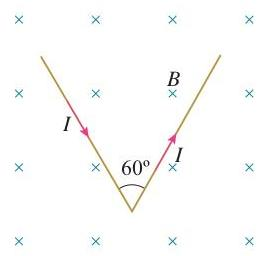
\includegraphics[max width=0.3\textwidth]{images/01910e72-c5b7-7ed5-a6d4-fb3a5faefc32_26_747258.jpg}
\end{center}

图 1-3

5. 一束粒子中有带正电的, 有带负电的, 还有不带电的。要想把它们分开, 可以用哪些办法?

6. 质子和 \(\alpha\) 粒子在同一匀强磁场中做半径相同的圆周运动。求质子的动能和 \(\alpha\) 粒子的动能之比。

7. 如图 1-4 所示,质量为 \({m}_{\mathrm{x}}\) 长为 \(l\) 的直导线用两绝缘细线悬挂于 \(O\text{、}{O}^{\prime }\) ,并处于匀强磁场中。当导线中通以沿 \(x\) 轴正方向的电流 \(I\) ,且导线保持静止时,悬线与竖直方向夹角为 \({\theta }_{ \circ }\) 有以下三种磁感应强度方向:

(1)沿 \(z\) 轴正方向; (2) 沿 \(y\) 轴正方向; (3)沿悬线向上。

请判断哪些是可能的, 可能时其磁感应强度大小是多少? 如果不可能, 请说明原因。

\begin{center}
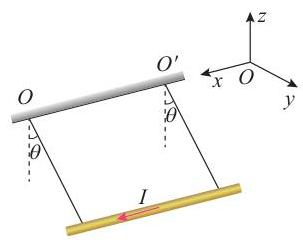
\includegraphics[max width=0.3\textwidth]{images/01910e72-c5b7-7ed5-a6d4-fb3a5faefc32_26_939137.jpg}
\end{center}

图 1-4

1. 如图 1-5 所示,金属杆 \({ab}\) 的质量为 \(m\) , 长为 \(l\) ,通过的电流为 \(I\) ,处在磁感应强度为 \(B\) 的匀强磁场中,磁场方向与导轨平面为 \(\theta\) 角斜向上,结果 \({ab}\) 静止于水平导轨上。

(1)求金属杆 \({ab}\) 受到的摩擦力。

(2)求金属杆对导轨的压力。

\begin{center}
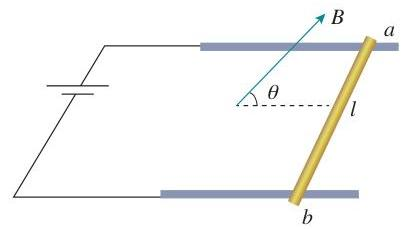
\includegraphics[max width=0.4\textwidth]{images/01910e72-c5b7-7ed5-a6d4-fb3a5faefc32_27_480802.jpg}
\end{center}

图 1-5

2. 如图 1-6 所示,宽为 \(l\) 的光滑导轨与水平面成 \(\alpha\) 角,质量为 \(m\) 、长为 \(l\) 的金属杆水平放置在导轨上。空间存在着匀强磁场, 当回路总电流为 \({I}_{1}\) 时,金属杆恰好能静止。

(1)磁感应强度 \(B\) 至少有多大? 此时方向如何?

(2)若保持 \(B\) 的大小不变而将 \(B\) 的方向改为竖直向上,应把回路总电流 \({I}_{2}\) 调到多大才能使金属杆保持静止?

\begin{center}
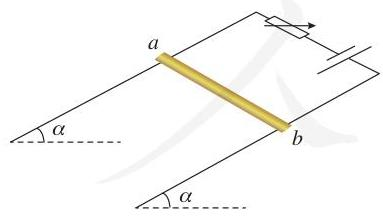
\includegraphics[max width=0.4\textwidth]{images/01910e72-c5b7-7ed5-a6d4-fb3a5faefc32_27_374731.jpg}
\end{center}

图 1-6

3. 利用学过的知识, 请你想办法把下面的带电粒子束分开: a. 速度不同的电子; b. 具有相同动能的质子和 \(\alpha\) 粒子 ( \(\alpha\) 粒子由两个质子和两个中子组成,质子与 \(\alpha\) 粒子的比荷不同)。

\section*{B 组}

4. 真空区域有宽度为 \(l\) 、磁感应强度为 \(B\) 的匀强磁场, 磁场方向如图 1-7 所示, \({MN}\) 、 \({PQ}\) 是磁场的边界。质量为 \(m\) 、电荷量为 \(q\) 的粒子 (不计重力) 沿着与 \({MN}\) 夹角 \(\theta\) 为 \({30}^{ \circ }\) 的方向射入磁场中,刚好没能从 \({PQ}\) 边界射出磁场。 求粒子射入磁场的速度大小及在磁场中运动的时间。

\begin{center}
\includegraphics[max width=0.2\textwidth]{images/01910e72-c5b7-7ed5-a6d4-fb3a5faefc32_27_322475.jpg}
\end{center}

图 1-7

5. 某一具有速度选择器的质谱仪原理如图 1-8 所示, \(\mathrm{A}\) 为粒子加速器,加速电压为 \({U}_{1}\) ; B 为速度选择器, 磁场与电场正交, 磁感应强度为 \({B}_{1}\) ,两板间距离为 \(d;\mathrm{C}\) 为偏转分离器,磁感应强度为 \({B}_{2}\) 。今有一质量为 \(m\) 、电荷量为 \(e\) 的正粒子 (不计重力), 经加速后, 该粒子恰能通过速度选择器, 粒子进入分离器后做匀速圆周运动。

(1)粒子的速度 \(v\) 为多少?

(2)速度选择器两板间电压 \({U}_{2}\) 为多少?

(3)粒子在 \({B}_{2}\) 磁场中做匀速圆周运动的半径 \(R\) 为多大?

\begin{center}
\includegraphics[max width=0.3\textwidth]{images/01910e72-c5b7-7ed5-a6d4-fb3a5faefc32_27_978805.jpg}
\end{center}

图 1-8

\section*{第二章}

\section*{电磁感应}

朝辞白帝彩云间,千里江陵一日还。

两岸猿声啼不住,轻舟已过万重山。

这首人们耳熟能详的唐诗,曾给我们带来多少愉悦和幻想呀! 如今, 诗人笔下的三峡, 不仅风景秀丽依然,更在为祖国的建设作着巨大的贡献。三峡水电站安装着 32 台巨型发电机, 总装机容量 2250 万千瓦。千年流淌的滚滚长江,正在焕发着青春。

电厂里巨大的发电机怎么会发出这么多电来? 磁生电有什么规律呢? 这一章我们将进一步去认识电与磁的规律。

在他 (法拉第) 的眼中, 华丽的宫廷和布拉顿高原上的雷雨比起来, 算得了什么? 皇家的一切器具和落日比较起来, 又算什么? 我之所以说出雷雨和落日, 因为这些现象在他的心里, 都可以挑起一种狂喜……

一丁铎尔 \({}^{\left( 1\right) }\)

\section*{1 楞次定律}

\section*{问题}

\begin{center}
\includegraphics[max width=0.3\textwidth]{images/01910e72-c5b7-7ed5-a6d4-fb3a5faefc32_29_377489.jpg}
\end{center}

线圈与电流表相连, 把磁体的某一个磁极向线圈中插入、从线圈中抽出时, 电流表的指针发生了偏转, 但两种情况下偏转的方向不同, 这说明感应电流的方向并不相同。感应电流的方向与哪些因素有关?

\section*{影响感应电流方向的因素}

我们知道, 穿过闭合回路的磁通量变化是产生感应电流的条件, 看来感应电流的方向可能与磁通量的变化有关。

\section*{实验}

\section*{探究影响感应电流方向的因素}

在上面的实验中,条形磁体的 \(\mathrm{N}\) 极或 \(\mathrm{S}\) 极插入闭合线圈时,穿过线圈的磁通量增大, \(\mathrm{N}\) 极或 \(\mathrm{S}\) 极抽出时,穿过线圈的磁通量减小。想一想,感应电流的方向与磁通量的变化之间有什么关系呢?

\customfootnote{

① 丁铎尔 (John Tyndall, 1820 -1893), 英国物理学家, 法拉第的学生和朋友,《作为一个发现者的法拉第》一书的作者。

}

在纸上画出上面实验的草图, 记录磁极运动的四种情况 (图 2.1-1)。根据实验结果, 分别标出不同情况下磁体的 \(\mathrm{N}\) 极、 \(\mathrm{S}\) 极的运动方向以及感应电流的方向。

\begin{center}
\includegraphics[max width=0.9\textwidth]{images/01910e72-c5b7-7ed5-a6d4-fb3a5faefc32_30_823891.jpg}
\end{center}

图 2.1-1 研究感应电流方向的实验记录

实验现象表明, 穿过线圈的磁通量都在增大时, 如果磁场方向不同 (图 2.1-1 甲、 乙), 感应电流的方向并不相同。而穿过线圈的磁通量都减小时, 如果磁场的方向不同 (图 2.1-1 丙、丁), 感应电流的方向也不同。看来, 实验并不能直接显示出感应电流的方向与磁通量变化的关系。

感应电流的方向与磁通量变化不容易建立起直接的联系, 那么应该如何转换一个角度来研究这一问题呢?

进一步分析可以想到, 磁体周围存在磁场, 感应电流也会产生磁场。感应电流磁场的磁通量与磁体磁场的磁通量有没有联系呢?

由于线圈的横截面积是不变的, 磁通量的变化可以用磁场的变化来体现。感应电流的方向与磁场的方向有关, 我们应该选择磁体的磁场和感应电流的磁场进行分析。

下面用表格来比较图 2.1-1 中的信息。由于这几幅图标出了感应电流的方向, 所以根据右手螺旋定则就能判定感应电流的磁场方向。

我们分别研究穿过线圈的磁通量增大和减小的情况。

\section*{表 1 磁通量增大时的情况}

\begin{center}
\adjustbox{max width=\textwidth}{
\begin{tabular}{|c|c|c|c|}
\hline
图号 & 磁体磁场的方向 & 感应电流的方向 & 感应电流的磁场方向 \\
\hline
甲 & 向下 & 逆时针(俯视) & 向上 \\
\hline
乙 & 向上 & 顺时针(俯视) & 向下 \\
\hline
\end{tabular}
}
\end{center}

比较表 1 中的数据, 可以发现, 当穿过线圈的磁通量增大时, 感应电流的磁场与磁体的磁场方向相反, 阻碍磁通量的增加。

表 2 磁通量减小时的情况

\begin{center}
\adjustbox{max width=\textwidth}{
\begin{tabular}{|c|c|c|c|}
\hline
图号 & 磁体的磁场方向 & 感应电流的方向 & 感应电流的磁场方向 \\
\hline
丙 & \phantom{X} & \phantom{X} & \phantom{X} \\
\hline
丁 & \phantom{X} & \phantom{X} & \phantom{X} \\
\hline
\end{tabular}
}
\end{center}

根据实验结果填写表 2 , 比较表 2 中的数据。当穿过线圈的磁通量减小时, 感应电流的磁场与磁体磁场的方向是相同的, 还是相反的? 是有助于磁通量的减小, 还是阻碍了磁通量的减小?

概括以上的实验结果, 能得出什么结论?

\section*{楞次定律}

1834 年, 俄国物理学家楞次在分析了许多实验事实后, 得到了关于感应电流方向的规律: 感应电流具有这样的方向,即感应电流的磁场总要阻碍引起感应电流的磁通量的变化。 这就是楞次定律 (Lenz's law )。

感应电流沿着楞次定律所述的方向, 是能量守恒定律的必然结果。我们知道, 由于电阻的存在, 感应电流在闭合回路中流动时将产生热量。根据能量守恒定律, 能量不可能无中生有, 这部分热量只可能从其他形式的能量转化而来。在上述实验中, 把磁极插入线圈或从线圈内抽出时, 推力或拉力都必须做机械功, 做功过程中消耗的机械能转化成感应电流的电能。

\section*{电考与讨论}

\begin{center}
\includegraphics[max width=0.3\textwidth]{images/01910e72-c5b7-7ed5-a6d4-fb3a5faefc32_31_612489.jpg}
\end{center}

图 2.1-2 磁体靠近或远离铝环

如图 2.1-2, 用绳吊起一个铝环, 用磁体的任意一极去靠近铝环, 会产生什么现象? 把磁极从靠近铝环处移开, 会产生什么现象? 解释发生的现象。

用楞次定律可以判定感应电流的方向。下面我们通过实例来了解处理这类问题的思路。

\section*{【例题 1】}

法拉第最初发现电磁感应现象的实验如图 2.1-3 所示。 软铁环上绕有 \(\mathrm{M}\text{、}\mathrm{\;N}\) 两个线圈,当线圈 \(\mathrm{M}\) 电路中的开关断开的瞬间, 线圈 \(\mathrm{N}\) 中的感应电流沿什么方向?

\begin{center}
\includegraphics[max width=0.3\textwidth]{images/01910e72-c5b7-7ed5-a6d4-fb3a5faefc32_32_496896.jpg}
\end{center}

图 2.1-3

分析与解答 首先明确, 我们用楞次定律研究的对象是线圈 \(\mathrm{N}\) 和电流表组成的闭合导体回路。

线圈 \(\mathrm{M}\) 中的电流在铁环中产生的磁感线是顺时针方向的 (图 2.1-4),这些磁感线穿过线圈 \(\mathrm{N}\) 的方向是向下的,即线圈 \(\mathrm{N}\) 中原磁场 \({B}_{0}\) 的方向是向下的。

\begin{center}
\includegraphics[max width=0.3\textwidth]{images/01910e72-c5b7-7ed5-a6d4-fb3a5faefc32_32_920278.jpg}
\end{center}

图 2.1-4

开关断开的瞬间,铁环中的磁场迅速减弱,线圈 \(\mathrm{N}\) 中的磁通量减小。

感应电流的磁场 \({B}_{\mathrm{i}}\) (图 2.1-4 中没有标出) 要阻碍磁通量的减小,所以, \({B}_{\mathrm{i}}\) 的方向与 \({B}_{0}\) 的方向相同,即线圈 \(\mathrm{N}\) 中 \({B}_{\mathrm{i}}\) 的方向也是向下的。

根据右手螺旋定则,由 \({B}_{\mathrm{i}}\) 的方向判定,线圈 \(\mathrm{N}\) 中感应电流 \({I}_{\mathrm{i}}\) 应沿图 2.1-4 所示的方向。

\section*{【例题 2】}

如图 2.1-5 所示,在通有电流 \(I\) 的长直导线附近有一个矩形线圈 \({ABCD}\) ,线圈与导线始终在同一个平面内。线圈在导线的一侧,垂直于导线左右平移时,其中产生了 \(A \rightarrow B \rightarrow C \rightarrow D \rightarrow A\) 方向的电流。已知距离载流直导线较近的位置磁场较强。请判断: 线圈在向哪个方向移动?

\begin{center}
\includegraphics[max width=0.2\textwidth]{images/01910e72-c5b7-7ed5-a6d4-fb3a5faefc32_32_748696.jpg}
\end{center}

图 2.1-5

分析与解答 选择矩形线圈为研究对象, 画出通电直导线一侧的磁感线分布图 (图 2.1-6), 磁感线方向垂直纸面向里,用 “ \(\times\) ” 表示。已知矩形线圈中感应电流的方向是 \(A \rightarrow B \rightarrow\) \(C \rightarrow D \rightarrow A\) ,根据右手螺旋定则,感应电流的磁场方向是垂直纸面向外的 (即指向读者的, 用矩形中心的圆点 “·” 表示)。

\begin{center}
\includegraphics[max width=0.2\textwidth]{images/01910e72-c5b7-7ed5-a6d4-fb3a5faefc32_32_970453.jpg}
\end{center}

图 2.1-6

根据楞次定律, 感应电流的磁场应该是阻碍穿过线圈的磁通量变化的。现在已经判明感应电流的磁场从纸面内向外指向读者, 是跟原来磁场的方向相反的。因此线圈移动时通过它的磁通量一定是在增大。这说明线圈在向左移动。

\section*{右手定则}

我们用楞次定律进行分析, 看一看当闭合导体回路的一部分做切割磁感线的运动时, 怎样判定感应电流的方向。

\section*{电考与讨论}

\begin{center}
\includegraphics[max width=0.3\textwidth]{images/01910e72-c5b7-7ed5-a6d4-fb3a5faefc32_33_893522.jpg}
\end{center}

图 2.1-7 判定感应电流的方向

在图 2.1-7 中, 假定导体棒 \({CD}\) 向右运动。

1. 我们研究的是哪个闭合导体回路?

2. 当导体棒 \({CD}\) 向右运动时,穿过这个闭合导体回路的磁通量是增大还是减小?

3. 感应电流的磁场应该是沿哪个方向的?

4. 导体棒 \({CD}\) 中的感应电流是沿哪个方向的?

\begin{center}
\includegraphics[max width=0.2\textwidth]{images/01910e72-c5b7-7ed5-a6d4-fb3a5faefc32_33_691887.jpg}
\end{center}

图 2.1-8 右手定则

可以用右手的手掌和手指的方向来判断导线切割磁感线时产生的感应电流的方向 (图 2.1-8), 即: 伸开右手, 使拇指与其余四个手指垂直,并且都与手掌在同一个平面内; 让磁感线从掌心进入,并使拇指指向导线运动的方向, 这时四指所指的方向就是感应电流的方向。这就是更便于判定导线切割磁感线时感应电流方向的右手定则 (righthand rule )。

\section*{科学方法}

\section*{归纳推理}

归纳推理是从一类事物的部分对象所具有的某种属性出发, 推理出这类事物的所有对象都具有共同属性的推理方法, 也就是由具体结论推理出一般规律的方法。楞次定律的得出就运用了归纳推理。通过研究不同磁极插入和拔出线圈等的实验现象, 逐步归纳推理得出反映感应电流方向的规律。与演绎推理不同的是, 归纳推理是从物理现象出发研究问题, 而演绎推理则是由已知物理规律出发研究问题。

\section*{练习与应用}

1. 在图 2.1-9 中, 线圈 \(\mathrm{M}\) 和线圈 \(\mathrm{P}\) 绕在同一个铁芯上。

(1)当闭合开关 \(\mathrm{S}\) 的一瞬间,线圈 \(\mathrm{P}\) 中感应电流的方向如何?

(2)当断开开关 \(\mathrm{S}\) 的一瞬间,线圈 \(\mathrm{P}\) 中感应电流的方向如何?

\begin{center}
\includegraphics[max width=0.3\textwidth]{images/01910e72-c5b7-7ed5-a6d4-fb3a5faefc32_34_847537.jpg}
\end{center}

图 2.1-9

2. 在图 2.1-10 中 \({CDEF}\) 是金属框,框内存在着如图所示的匀强磁场。当导体 \({MN}\) 向右移动时, 请用楞次定律判断 \({MNDC}\) 和 \({MNEF}\) 两个电路中感应电流的方向。

\begin{center}
\includegraphics[max width=0.3\textwidth]{images/01910e72-c5b7-7ed5-a6d4-fb3a5faefc32_34_495440.jpg}
\end{center}

图 2.1-10

3. 如图 2.1-11 所示,导线 \({AB}\) 与 \({CD}\) 平行。试判断在闭合与断开开关 \(\mathrm{S}\) 时,导线 \({CD}\) 中感应电流的方向, 说明你判断的理由。

\begin{center}
\includegraphics[max width=0.3\textwidth]{images/01910e72-c5b7-7ed5-a6d4-fb3a5faefc32_34_829824.jpg}
\end{center}

图 2.1-11

4. 如图 2.1-12 所示, 在水平放置的条形磁体的 \(\mathrm{N}\) 极附近,一个闭合线圈竖直向下运动并始终保持水平。在位置 \(B,\mathrm{\;N}\) 极附近的磁感线正好与线圈平面平行, \(A\text{、}B\) 之间和 \(B\text{、}C\) 之间的距离都比较小。试判断线圈在位置 \(A\text{、}B\text{、}C\) 时感应电流的方向, 说明你判断的理由。

\begin{center}
\includegraphics[max width=0.5\textwidth]{images/01910e72-c5b7-7ed5-a6d4-fb3a5faefc32_34_284901.jpg}
\end{center}

图 2.1-12

5. 图 2.1-13 中的 \(\mathrm{A}\) 和 \(\mathrm{B}\) 都是铝环, \(\mathrm{A}\) 环是闭合的, B 环是断开的, 横梁可以绕中间的支点转动。某人在实验时, 用磁体的任意一极移近 A 环, A 环都会被推斥, 把磁体远离 A 环, A 环又会被磁体吸引。但磁体移近或远离 B 环时, 却没有发现与 A 环相同的现象。这是为什么?

\begin{center}
\includegraphics[max width=0.4\textwidth]{images/01910e72-c5b7-7ed5-a6d4-fb3a5faefc32_34_865294.jpg}
\end{center}

图 2.1-13

\section*{2 法拉第电磁感应定律}

\section*{问题}

\begin{center}
\includegraphics[max width=0.3\textwidth]{images/01910e72-c5b7-7ed5-a6d4-fb3a5faefc32_35_395030.jpg}
\end{center}

穿过闭合导体回路的磁通量发生变化, 闭合导体回路中就有感应电流。感应电流的大小跟哪些因素有关呢?

在用导线切割磁感线产生感应电流的实验中, 导线切割磁感线的速度越快、磁体的磁场越强, 产生的感应电流就越大。在向线圈中插入条形磁体的实验中, 磁体的磁场越强、插入的速度越快, 产生的感应电流就越大。这些现象向我们提示, 当回路中的电阻一定时, 感应电流的大小可能与磁通量变化的快慢有关, 而磁通量变化的快慢可以用磁通量的变化率表示。也就是说, 感应电流的大小与磁通量的变化率有关。

\section*{做一做}

实验装置如图 2.2-1 所示, 线圈的两端与电压表相连。 将强磁体从长玻璃管上端由静止下落, 穿过线圈。分别使线圈距离上管口 \({20}\mathrm{\;{cm}}\text{、}{30}\mathrm{\;{cm}}\text{、}{40}\mathrm{\;{cm}}\) 和 \({50}\mathrm{\;{cm}}\) ,记录电压表的示数以及发生的现象。

\begin{center}
\includegraphics[max width=0.2\textwidth]{images/01910e72-c5b7-7ed5-a6d4-fb3a5faefc32_35_388542.jpg}
\end{center}

图 2.2-1

分别改变线圈的匝数、磁体的强度, 重复上面的实验, 得出定性的结论。

\section*{电磁感应定律}

电路中有感应电流, 就一定有电动势。如果电路没有闭合, 这时虽然没有感应电流, 电动势依然存在。

在电磁感应现象中产生的电动势叫作感应电动势 (induction electromotive force)。产生感应电动势的那部分导体就相当于电源。

德国物理学家纽曼、韦伯在对理论和实验资料进行严格分析后, 于 1845 年和 1846 年先后指出: 闭合电路中感应电动势的大小, 跟穿过这一电路的磁通量的变化率成正比。因法拉第对电磁感应现象研究的巨大贡献, 后人称之为法拉第电磁感应定律 (Faraday's law of electromagnetic induction )。

如果在极短的时间 \({\Delta t}\) 内,磁通量的变化量为 \({\Delta \Phi }\) ,磁通量的变化率就是 \(\frac{\Delta \Phi }{\Delta t}\) 。用 \(E\) 表示闭合电路中的感应电动势, 那么电磁感应定律就可以表示为

\[
E = k\frac{\Delta \Phi }{\Delta t}
\]

式中 \(k\) 是比例常量。在国际单位制中,电动势 \(E\) 的单位是伏 ( V )、磁通量 \(\Phi\) 的单位是韦伯 ( Wb ) 、时间 \(t\) 的单位是秒 ( s ),这时 \(k = 1\) 。于是

\[
E = \frac{\Delta \Phi }{\Delta t} \tag{1}
\]

闭合电路常常是一个匝数为 \(n\) 的线圈,而且穿过每匝线圈的磁通量总是相同的。由于这样的线圈可以看成是由 \(n\) 个单匝线圈串联而成的,因此整个线圈中的感应电动势是单匝线圈的 \(n\) 倍,即

\[
E = n\frac{\Delta \Phi }{\Delta t} \tag{2}
\]

\begin{mdframed}

这几个公式只表示感应电动势的大小。至于感应电流的方向, 可以用上节学到的楞次定律判定。

\end{mdframed}

\section*{导线切割磁感线时的感应电动势}

\begin{center}
\includegraphics[max width=0.3\textwidth]{images/01910e72-c5b7-7ed5-a6d4-fb3a5faefc32_36_708283.jpg}
\end{center}

图 2.2-2 计算导线切割磁感线时的感应电动势

根据法拉第电磁感应定律, 只要知道磁通量的变化率, 就可以算出感应电动势。一种情况是, 导线做切割磁感线运动而使磁通量变化, 这时法拉第电磁感应定律可以表示为一种更简单、更便于应用的形式。

如图 2.2-2 所示,把矩形线框 \({CDMN}\) 放在磁感应强度为 \(B\) 的匀强磁场里,线框平面跟磁感线垂直。设线框可动部分导体棒 \({MN}\) 的长度为 \(l\) ,它以速度 \(v\) 向右运动,在 \({\Delta t}\) 时间内,由原来的位置 \({MN}\) 移到 \({M}_{1}{N}_{1}\) 。这个过程中线框的面积变化量是

\[
{\Delta S} = {lv\Delta t}
\]

穿过闭合电路的磁通量的变化量则是

\[
{\Delta \Phi } = {B\Delta S} = {Blv\Delta t}
\]

根据法拉第电磁感应定律, \(E = \frac{\Delta \Phi }{\Delta t}\) ,由此求得感应电动势

\[
E = {Blv}
\]

在国际单位制中,磁感应强度 \(B\) 、导线长度 \(l\) 、速度 \(v\) 的单位分别是特斯拉 ( \(\mathrm{T}\) )、米 \(\left( \mathrm{m}\right)\) 、米每秒 \(\left( {\mathrm{m}/\mathrm{s}}\right) ,E\) 的单位是伏 \(\left( \mathrm{V}\right)\) 。

如果导线的运动方向与导线本身是垂直的, 但与磁感线方向有一个夹角 \(\theta\) (图 2.2-3),速度 \(v\) 可以分解为两个分量: 垂直于磁感线的分量 \({v}_{1} = v\sin \theta\) 和平行于磁感线的分量 \({v}_{2} = v\cos {\theta }_{ \circ }\) 后者不切割磁感线,不产生感应电动势。 前者切割磁感线, 产生的感应电动势为

\[
E = {Bl}{v}_{1}
\]

考虑到 \({v}_{1} = v\sin \theta\) ,因此

\[
E = {Blv}\sin \theta
\]

\begin{center}
\includegraphics[max width=0.4\textwidth]{images/01910e72-c5b7-7ed5-a6d4-fb3a5faefc32_37_796293.jpg}
\end{center}

图 2.2-3 导线运动方向不与磁感线垂直时的情况

\section*{思考与讨论}

\begin{mdframed}

\begin{center}
\includegraphics[max width=0.2\textwidth]{images/01910e72-c5b7-7ed5-a6d4-fb3a5faefc32_38_341416.jpg}
\end{center}

图 2.2-4 导体棒做切割磁感线运动

\end{mdframed}

如图 2.2-4,导体棒 \({CD}\) 在匀强磁场中运动。自由电荷会随着导体棒运动, 并因此受到洛伦兹力。导体棒中自由电荷相对于纸面的运动大致沿什么方向? 为了方便, 可以认为导体棒中的自由电荷是正电荷。

导体棒一直运动下去, 自由电荷是否总会沿着导体棒运动? 为什么? 导体棒哪端的电势比较高?

以上讨论不必考虑自由电荷的热运动。

一段导线在做切割磁感线的运动时相当于一个电源, 通过上面的分析可以看到, 这时的非静电力与洛伦兹力有关。 在图 2.2-2 中, 由于导体棒运动产生感应电动势, 电路中有电流通过, 导体棒在运动过程中会受到安培力的作用。可以判断, 安培力的方向与推动导体棒运动的力的方向是相反的。这时即使导体棒做匀速运动, 推力也做功。如果没有推力的作用, 导体棒将克服安培力做功而消耗本身的机械能。

\begin{mdframed}

\begin{itemize}
\item 如果感应电动势是由于导体运动而产生的, 它也叫作动生电动势。
\end{itemize}

\end{mdframed}

\section*{(练习与应用}

1. 有一个 1000 匝的线圈,在 \({0.4}\mathrm{\;s}\) 内通过它的磁通量从 \({0.02}\mathrm{\;{Wb}}\) 增加到 \({0.09}\mathrm{\;{Wb}}\) ,求线圈中的感应电动势。如果线圈的电阻是 \({10\Omega }\) , 把一个电阻为 \({990\Omega }\) 的电热器连接在它的两端, 通过电热器的电流是多大?

2. 当航天飞机在环绕地球的轨道上飞行时, 从中释放一颗卫星, 卫星与航天飞机速度相同, 两者用导电缆绳相连。这种卫星称为绳系卫星, 利用它可以进行多种科学实验。

现有一绳系卫星在地球赤道上空沿东西方向运行。卫星位于航天飞机的正上方, 它与航天飞机之间的距离是 \({20.5}\mathrm{\;{km}}\) ,卫星所在位置的地磁场 \(B = {4.6} \times {10}^{-5}\mathrm{\;T}\) ,沿水平方向由南向北。如果航天飞机和卫星的运行速度都是 \({7.6}\mathrm{\;{km}}/\mathrm{s}\) ,求缆绳中的感应电动势。

3. 动圈式扬声器的结构如图 2.2-5 所示。 线圈圆筒安放在永磁体磁极间的空隙中, 能够在空隙中左右运动。音频电流通进线圈, 安培力使线圈左右运动。纸盆与线圈连接, 随着线圈振动而发声。

\begin{center}
\includegraphics[max width=0.3\textwidth]{images/01910e72-c5b7-7ed5-a6d4-fb3a5faefc32_38_178091.jpg}
\end{center}

图 2.2-5

这样的扬声器能不能当作话筒使用? 也就是说, 如果我们对着纸盆说话, 扬声器能不能把声音变成相应的电流? 为什么?

4. 如图 2.2-6,矩形线圈在匀强磁场中绕 \(O{O}^{\prime }\) 轴匀速转动时, 线圈中的感应电动势是否变化? 为什么? 设线圈的两个边长分别是 \({l}_{1}\) 和 \({l}_{2}\) ,转动时角速度是 \(\omega\) ,磁场的磁感应强度为 \(B\) 。试证明: 在图示位置时, 线圈中的感应电动势为 \(E = {BS\omega }\) ,式中 \(S = {l}_{1}{l}_{2}\) ,为线圈面积。

\begin{center}
\includegraphics[max width=0.2\textwidth]{images/01910e72-c5b7-7ed5-a6d4-fb3a5faefc32_39_661803.jpg}
\end{center}

图 2.2-6

5. 图 2.2-7 是电磁流量计的示意图。圆管由非磁性材料制成, 空间有匀强磁场。当管中的导电液体流过磁场区域时,测出管壁上 \(M\) 、 \(N\) 两点间的电势差 \(U\) ,就可以知道管中液体的流量 \(Q\) ——单位时间内流过管道横截面的液体体积。已知管的直径为 \(d\) ,磁感应强度为 \(B\) , 试推出 \(Q\) 与 \(U\) 关系的表达式。假定管中各处液体的流速相同。

\begin{center}
\includegraphics[max width=0.5\textwidth]{images/01910e72-c5b7-7ed5-a6d4-fb3a5faefc32_39_506958.jpg}
\end{center}

图 2.2-7

电磁流量计的管道内没有任何阻碍液体流动的结构, 所以常用来测量高黏度及强腐蚀性流体的流量。它的优点是测量范围宽、反应快、易与其他自动控制装置配套。

6. 一长为 \(l\) 的导体棒在磁感应强度为 \(B\) 的匀强磁场中绕其一端以角速度 \(\omega\) 在垂直于磁场的平面内匀速转动 (图 2.2-8),求 \({ab}\) 两端产生的感应电动势。

\begin{center}
\includegraphics[max width=0.4\textwidth]{images/01910e72-c5b7-7ed5-a6d4-fb3a5faefc32_39_917581.jpg}
\end{center}

图 2.2-8

\section*{3 涡流、电磁阻尼和电磁驱动}

\section*{问题}

在电磁炉的炉盘下有一个线圈。电磁炉工作时, 它的盘面并不发热, 在炉盘上面放置铁锅, 铁锅会发热。你知道这是为什么吗?

\section*{电磁感应现象中的感生电场}

\begin{mdframed}

如果感应电动势是由感生电场产生的, 它也叫作感生电动势。

\end{mdframed}

麦克斯韦认为, 磁场变化时会在空间激发一种电场。 这种电场与静电场不同, 它不是由电荷产生的, 我们把它叫作感生电场 (induced electric field)。如果此刻空间存在闭合导体, 导体中的自由电荷就会在感生电场的作用下做定向运动, 产生感应电流, 也就是说导体中产生了感应电动势。

\begin{center}
\includegraphics[max width=0.4\textwidth]{images/01910e72-c5b7-7ed5-a6d4-fb3a5faefc32_40_382828.jpg}
\end{center}

图 2.3-1 电子感应加速器

现代科学研究中常要用到高速电子, 电子感应加速器就是利用感生电场使电子加速的设备。它的基本原理如图 2.3-1 甲所示, 上、下为电磁铁的两个磁极, 磁极之间有一个环形真空室, 电子在真空室中做圆周运动。电磁铁线圈中电流的大小、方向可以变化, 产生的感生电场使电子加速。

从图 2.3-1 甲中可以看到, 磁场方向由下向上, 如果从上向下看 ( \({2.3} - 1\) 乙),电子沿逆时针方向运动。电子带负电, 它在电场中受力的方向与电场方向相反。所以为使电子加速, 产生的电场应沿顺时针方向。根据楞次定律, 为使真空室中产生顺时针方向的感生电场, 磁场应该由弱变强。也就是说, 为使电子加速, 电磁铁线圈中的电流应该由小变大。

\section*{涡流}

当某线圈中的电流随时间变化时, 由于电磁感应, 附近的另一个线圈中可能会产生感应电流。实际上, 这个线圈附近的任何导体, 如果穿过它的磁通量发生变化, 导体内都会产生感应电流, 如图 2.3-2 中的虚线所示。如果用图表示这样的感应电流, 看起来就像水中的漩涡, 所以把它叫作涡电流, 简称涡流 (eddy current)。

\begin{center}
\includegraphics[max width=0.3\textwidth]{images/01910e72-c5b7-7ed5-a6d4-fb3a5faefc32_41_829650.jpg}
\end{center}

图2.3-2 导体中产生涡流

\begin{center}
\includegraphics[max width=0.3\textwidth]{images/01910e72-c5b7-7ed5-a6d4-fb3a5faefc32_41_119655.jpg}
\end{center}

图 2.3-3 真空冶炼炉

金属块中的涡流会产生热量。用来冶炼合金钢的真空冶炼炉 (图 2.3-3), 炉外有线圈, 线圈中通入迅速变化的电流, 炉内的金属中产生涡流。涡流产生的热量使金属熔化。 利用涡流冶炼金属的优点是, 整个过程可以在真空中进行, 能防止空气中的杂质进入金属, 可以冶炼高质量的合金。

\begin{center}
\includegraphics[max width=0.3\textwidth]{images/01910e72-c5b7-7ed5-a6d4-fb3a5faefc32_41_193077.jpg}
\end{center}

图 2.3-4 电磁炉加热食物

本节问题中, 迅速变化的电流通过电磁炉面板下方的线圈时, 线圈周围产生迅速变化的磁场, 变化的磁场使面板上方的铁锅底部产生涡流, 铁锅迅速发热, 从而达到加热食物的目的 (图2.3-4)。

电动机、变压器的线圈都绕在铁芯上。线圈中流过变化的电流, 在铁芯中产生的涡流使铁芯发热, 浪费了能量, 还可能损坏电器。因此, 我们要想办法减小涡流。途径之一是增大铁芯材料的电阻率, 常用的铁芯材料是硅钢, 它的电阻率比较大。另一个途径就是用互相绝缘的硅钢片叠成的铁芯来代替整块硅钢铁芯 (图 2.3-5 )。

一种探测地雷的探雷器是利用涡流工作的。士兵手持一个长柄线圈在地面扫过 (图 2.3-6), 线圈中有变化着的电流。如果地下埋着金属物品,金属中会感应出涡流,涡流的磁场反过来影响线圈中的电流, 使仪器报警。这种探雷器可以用来探测金属壳的地雷或有较大金属零件的地雷。

\begin{center}
\includegraphics[max width=0.3\textwidth]{images/01910e72-c5b7-7ed5-a6d4-fb3a5faefc32_42_881697.jpg}
\end{center}

图 2.3-5 用硅钢片做变压器的铁芯

\begin{center}
\includegraphics[max width=0.3\textwidth]{images/01910e72-c5b7-7ed5-a6d4-fb3a5faefc32_42_793802.jpg}
\end{center}

图 2.3-6 探雷

机场、车站和重要活动场所的安检门可以探测人身携带的金属物品, 道理是一样的。

\section*{电磁阻尼}

\section*{电考与讨论}

如图 2.3-7 所示, 一个单匝线圈落入磁场中, 分析它在图示位置时感应电流的方向和所受安培力的方向。安培力对线圈的运动有什么影响?

磁电式仪表的线圈常常用铝框做骨架, 把线圈绕在铝框上, 指针也固定在铝框上 (图 2.3-8 )。假定仪表工作时指针向右转动, 铝框中的感应电流沿什么方向? 由于铝框转动时其中有感应电流, 铝框要受到安培力。安培力是沿什么方向的? 安培力对铝框的转动产生什么影响?

\begin{center}
\includegraphics[max width=0.2\textwidth]{images/01910e72-c5b7-7ed5-a6d4-fb3a5faefc32_42_819012.jpg}
\end{center}

图 2.3-7

\begin{center}
\includegraphics[max width=0.4\textwidth]{images/01910e72-c5b7-7ed5-a6d4-fb3a5faefc32_42_595309.jpg}
\end{center}

图 2.3-8

当导体在磁场中运动时, 感应电流会使导体受到安培力, 安培力的方向总是阻碍导体的运动, 这种现象称为电磁阻尼。

\section*{做一做}

取一只微安表, 用手晃动表壳, 观察表针相对表盘摆动的情况。用导线把微安表的两个接线柱连在一起 (图 2.3-9), 再次晃动表壳, 表针相对表盘的摆动情况与刚才有什么不同? 怎样解释这种差别? 为什么灵敏电流表在运输时总要用导体把两个接线柱连在一起?

连接两个

\begin{center}
\includegraphics[max width=0.2\textwidth]{images/01910e72-c5b7-7ed5-a6d4-fb3a5faefc32_43_197660.jpg}
\end{center}

接线柱的导线

图 2.3-9

\section*{电磁驱动}

\section*{演示}

\begin{center}
\includegraphics[max width=0.2\textwidth]{images/01910e72-c5b7-7ed5-a6d4-fb3a5faefc32_43_358698.jpg}
\end{center}

图 2.3-10 铝框的运动

\section*{观察铝框的运动}

如图 2.3-10 所示, 一个铝框放在蹄形磁体的两个磁极间, 可以绕支点自由转动。转动磁体, 观察铝框的运动。 怎样解释铝框的运动?

如果磁场相对于导体转动, 在导体中会产生感应电流, 感应电流使导体受到安培力的作用, 安培力使导体运动起来, 这种作用常常称为电磁驱动。

交流感应电动机就是利用电磁驱动的原理工作的。配置的三个线圈连接到三相电源上, 就能产生类似上面演示实验中的旋转磁场, 磁场中的导线框也就随着转动 (图 2.3-11)。 就这样, 电动机 (图 2.3-12) 把电能转化成机械能。

\begin{center}
\includegraphics[max width=0.3\textwidth]{images/01910e72-c5b7-7ed5-a6d4-fb3a5faefc32_43_577212.jpg}
\end{center}

图 2.3-11 产生旋转磁场的装置

\begin{center}
\includegraphics[max width=0.3\textwidth]{images/01910e72-c5b7-7ed5-a6d4-fb3a5faefc32_43_698949.jpg}
\end{center}

图 2.3-12 电动机

1. 有一个铜盘, 轻轻拨动它, 能长时间地绕轴自由转动。如果在转动时把蹄形磁体的两极放在铜盘的边缘, 但并不与铜盘接触 (图 2.3-13 ), 铜盘就能在较短的时间内停止。分析这个现象产生的原因。

2. 如图 2.3-14 所示, 弹簧上端固定, 下端悬挂一个磁体。将磁体托起到某一高度后放开, 磁体能上下振动较长时间才停下来。如果在磁体下端放一个固定的闭合线圈, 使磁极上下振动时穿过它, 磁体就会很快地停下来。分析这个现象的产生原因, 并说明此现象中能量转化的情况。

\begin{center}
\includegraphics[max width=0.2\textwidth]{images/01910e72-c5b7-7ed5-a6d4-fb3a5faefc32_44_160166.jpg}
\end{center}

图 2.3-13

\begin{center}
\includegraphics[max width=0.2\textwidth]{images/01910e72-c5b7-7ed5-a6d4-fb3a5faefc32_44_773825.jpg}
\end{center}

图2.3-14

3. 在科技馆中常看到这样的表演: 一根长 \(1\mathrm{\;m}\) 左右的空心铝管竖直放置 (图 2.3-15 甲), 把一枚磁性比较强的小圆柱形永磁体从铝管上端放入管口, 圆柱直径略小于铝管的内径。根据一般经验,小圆柱自由下落 \(1\mathrm{\;m}\) 左右的时间不会超过 \({0.5}\mathrm{\;s}\) ,但把小圆柱从上端放入管中后, 过了许久它才从铝管下端落出。小圆柱在管内运动时, 没有感觉到它跟铝管内壁发生摩擦, 把小圆柱靠着铝管, 也不见它们相互吸引。是什么原因使小圆柱在铝管中缓慢下落呢? 如果换用一条有裂缝的铝管 (图 2.3-15 乙), 圆柱在铝管中的下落就变快了。这又是为什么?

\begin{center}
\includegraphics[max width=0.2\textwidth]{images/01910e72-c5b7-7ed5-a6d4-fb3a5faefc32_44_270743.jpg}
\end{center}

图 2.3-15

4. 人造卫星绕地球运行时, 轨道各处的地磁场的强弱并不相同, 因此, 金属外壳的人造地球卫星运行时, 外壳中总有感应电流。分析这一现象中的能量转化情形。它对卫星的运动可能产生怎样的影响?

5. 如图 2.3-16 所示, 水平放置的绝缘桌面上有一个金属圆环, 圆心的正上方有一个竖直的条形磁体。请通过分析形成以下结论: 条形磁体沿水平方向移动时, 金属圆环将受到水平方向运动的驱动力, 驱动力的方向跟条形磁体运动的方向相同。

\begin{center}
\includegraphics[max width=0.2\textwidth]{images/01910e72-c5b7-7ed5-a6d4-fb3a5faefc32_44_388143.jpg}
\end{center}

图 2.3-16

\section*{4 互感和自感}

\section*{问题}

\begin{center}
\includegraphics[max width=0.3\textwidth]{images/01910e72-c5b7-7ed5-a6d4-fb3a5faefc32_45_621765.jpg}
\end{center}

两个线圈 A、B 之间并没有导线相连, 线圈 A 与手机的音频输出端连接, 线圈 B 与扩音器的输入端连接。把线圈 \(\mathrm{A}\) 插入线圈 \(\mathrm{B}\) 时就能在扩音器上听见由手机输出的声音, 这是为什么?

\section*{互感现象}

在法拉第最初发现电磁感应现象的实验中, 两个线圈之间并没有导线相连, 但当一个线圈中的电流变化时, 它所产生的变化的磁场会在另一个线圈中产生感应电动势。 这种现象叫作互感 (mutual induction), 这种感应电动势叫作互感电动势。

利用互感现象可以把能量由一个线圈传递到另一个线圈, 因此互感在电工技术和电子技术中有广泛的应用。变压器就是利用互感现象制成的。

互感现象是一种常见的电磁感应现象, 它不仅可以发生于绕在同一铁芯上的两个线圈之间, 而且可以发生于任何两个相互靠近的电路之间。在电力工程和电子电路中, 互感现象有时会影响电路的正常工作, 这时要设法减小电路间的互感。

\section*{自感现象}

当一个线圈中的电流变化时, 它所产生的变化的磁场在线圈本身激发出感应电动势。这种现象称为自感 (self-induction), 由于自感而产生的感应电动势叫作自感电动势。

\section*{演示}

\section*{观察两个灯泡的发光情况}

在图 2.4-1 的电路中,两个灯泡 \({\mathrm{A}}_{1}\) 和 \({\mathrm{A}}_{2}\) 的规格相同, \({\mathrm{A}}_{1}\) 与线圈 \(L\) 串联后接到电源上, \({\mathrm{A}}_{2}\) 与可调电阻 \(R\) 串联后接到电源上。

先闭合开关 \(\mathrm{S}\) ,调节电阻 \(R\) ,使两个灯泡的亮度相同,再调节可调电阻 \({R}_{1}\) ,使它们都正常发光,然后断开开关 \(\mathrm{S}\) 。

重新接通电路。注意观察, 在开关闭合的时候两个灯泡的发光情况。

\begin{center}
\includegraphics[max width=0.3\textwidth]{images/01910e72-c5b7-7ed5-a6d4-fb3a5faefc32_46_661405.jpg}
\end{center}

图 2.4-1 开关闭合时观察灯泡的发光情况

\begin{center}
\includegraphics[max width=0.2\textwidth]{images/01910e72-c5b7-7ed5-a6d4-fb3a5faefc32_46_715610.jpg}
\end{center}

图2.4-2 感应电动势阻碍电流的增加

在图 2.4-1 的电路中, 闭合开关的瞬间, 电流从无到有, 线圈 \(L\) 中产生感应电动势。根据楞次定律,感应电动势会阻碍电流的增加 (图 2.4-2),所以灯泡 \({\mathrm{A}}_{1}\) 较慢地亮起来。

\section*{演示}

\section*{观察开关断开时灯泡的亮度}

按图 2.4-3 连接电路。先闭合开关使灯泡发光, 然后断开开关。注意观察开关断开时灯泡的亮度。演示前思考下列问题。

\begin{center}
\includegraphics[max width=0.3\textwidth]{images/01910e72-c5b7-7ed5-a6d4-fb3a5faefc32_46_540699.jpg}
\end{center}

图 2.4-3 开关断开时观察灯泡的亮度

1. 电源断开时,通过线圈 \(L\) 的电流减小,这时会出现感应电动势。感应电动势的作用是使线圈 \(L\) 中的电流减小得更快些还是更慢些?

2. 产生感应电动势的线圈可以看作一个电源, 它能向外供电。由于开关已经断开, 线圈提供的感应电流将沿什么路径流动?

3. 开关断开后, 通过灯泡的感应电流与原来通过它的电流方向是否一致?

4. 开关断开后, 通过灯泡的感应电流是否有可能比原来的电流更大? 为了使实验的效果更明显,对线圈 \(L\) 应该有什么要求?

\section*{做一做}

\section*{用电流传感器显示自感对电流的影响}

电流传感器的作用相当于一个电流表, 本书就用电流表的符号表示。传感器与计算机相结合不仅即时反映电流的迅速变化, 还能在屏幕上显示电流随时间变化的图像。

1. 按图 2.4-4 甲连接电路 (图 2.4-5 是实物连接图), 可以看到, 开关闭合时电流是逐渐增大的。为了说明这一点, 可以拆掉线圈 (图 2.4-4 乙) 再测一次, 看看两次测得的电流一时间图像有什么不同。

2. 将线圈 \(L\) 与电阻 \(R\) 并联后接到电池的两端 (电路与图 2.4-3 相仿),测量通过电阻 \(R\) 的电流,可以看到,开关断开前后通过电阻 \(R\) 的电流方向不同。

\begin{center}
\includegraphics[max width=0.2\textwidth]{images/01910e72-c5b7-7ed5-a6d4-fb3a5faefc32_47_970551.jpg}
\end{center}

图 2.4-4 显示通电时线圈对电流影响的实验

\begin{center}
\includegraphics[max width=0.5\textwidth]{images/01910e72-c5b7-7ed5-a6d4-fb3a5faefc32_47_140871.jpg}
\end{center}

图 2.4-5 实物连接图

变压器、电动机等设备中有匝数很多的线圈, 当电路中的开关断开时会产生很大的自感电动势, 使得开关中的金属片之间产生电火花, 烧蚀接触点, 甚至会引起人身伤害。因此, 切断这类电路时, 必须采用特制的安全开关, 避免出现电火花。

\section*{自感系数}

自感电动势也是感应电动势, 同样遵从法拉第电磁感应定律, 即

\[
E = n\frac{\Delta \Phi }{\Delta t}
\]

实验表明, 磁场的强弱正比于电流的强弱, 也就是说, 磁通量的变化正比于电流的变化。因此, 自感电动势正比于电流的变化率, 即

\[
E \propto \frac{\Delta I}{\Delta t}
\]

\begin{center}
\includegraphics[max width=0.3\textwidth]{images/01910e72-c5b7-7ed5-a6d4-fb3a5faefc32_48_748378.jpg}
\end{center}

图2.4-6 各种线圈

写成等式, 就是

\[
E = L\frac{\Delta I}{\Delta t}
\]

式中 \(L\) 是比例系数,叫作自感系数,简称自感或电感。它与线圈的大小、形状、匝数, 以及是否有铁芯等因素有关。 电感的单位是亨利 (henry), 简称亨, 符号是 \(\mathrm{H}\) 。常用的单位还有毫亨 \(\left( \mathrm{{mH}}\right)\) 、微亨 \(\left( {\mu \mathrm{H}}\right)\) 。图 2.4-6 中,不同的线圈,电感大小不同。

\section*{磁场的能量}

\begin{mdframed}

\begin{itemize}
\item 有时自感电动势会大于原来电路中的电源电动势。
\end{itemize}

\end{mdframed}

在图 2.4-3 的实验中, 开关断开后, 灯泡的发光还能维持一小段时间, 有时甚至会比开关断开之前更亮。这时灯泡的能量是从哪里来的?

开关断开以后, 线圈中的电流并未立即消失, 线圈中有电流, 有电流就有磁场, 能量储存在磁场中。当开关闭合时, 线圈中的电流从无到有, 其中的磁场也是从无到有, 这可以看作电源把能量输送给磁场, 储存在磁场中。

当线圈刚刚接通电源的时候, 自感电动势阻碍线圈中电流的增加; 当电源断开的时候, 自感电动势又阻碍线圈中电流的减小。线圈的自感系数越大, 这个现象越明显, 线圈能够体现电的 “惯性”。 练习与应用

1. 图 2.4-7 是一种延时继电器的示意图。铁芯上有两个线圈 \(\mathrm{A}\) 和 \(\mathrm{B}\) 。线圈 \(\mathrm{A}\) 跟电源连接, 线圈 \(\mathrm{B}\) 两端连在一起,构成一个闭合电路。在断开开关 \(\mathrm{S}\) 的时候,弹簧 \(\mathrm{K}\) 并不会立刻将衔铁 \(\mathrm{D}\) 拉起而使触头 \(\mathrm{C}\) (连接工作电路) 离开,而是过一小段时间后才执行这个动作。延时继电器就是因此而得名的。

\begin{center}
\includegraphics[max width=0.3\textwidth]{images/01910e72-c5b7-7ed5-a6d4-fb3a5faefc32_49_273532.jpg}
\end{center}

图 2.4-7

( 1 ) 请解释: 当开关 \(\mathrm{S}\) 断开后,为什么电磁体还会继续吸住衔铁一小段时间?

(2)如果线圈 \(\mathrm{B}\) 不闭合,是否会对延时效果产生影响? 为什么?

2. 李辉用多用电表的欧姆挡测量一个变压器线圈的电阻, 以判断它是否断路。刘伟为了使李辉测量方便, 没有注意操作的规范, 用两手分别握住线圈裸露的两端让李辉测量。测量时表针摆过了一定角度, 李辉由此确认线圈没有断路。正当李辉把多用电表的表笔与被测线圈脱离时, 刘伟突然惊叫起来, 觉得有电击感 (图 2.4-8)。李辉很奇怪, 用手摸摸线圈两端, 没有什么感觉, 再摸摸多用电表的两支表笔, 也没有什么感觉。这是什么原因?

\begin{center}
\includegraphics[max width=0.4\textwidth]{images/01910e72-c5b7-7ed5-a6d4-fb3a5faefc32_49_540627.jpg}
\end{center}

图 2.4-8

3. 如图 2.4-9 所示, \(L\) 是自感系数很大的线圈, 但其自身的电阻几乎为 0 。A 和 B 是两个相同的小灯泡。

( 1 ) 当开关 \(\mathrm{S}\) 由断开变为闭合时, \(\mathrm{A}\text{、}\mathrm{\;B}\) 两个灯泡的亮度将如何变化? 请作出解释。

(2)当开关 \(\mathrm{S}\) 由闭合变为断开时, \(\mathrm{A}\text{、}\mathrm{\;B}\) 两个灯泡的亮度又将如何变化? 请作出解释。

\begin{center}
\includegraphics[max width=0.4\textwidth]{images/01910e72-c5b7-7ed5-a6d4-fb3a5faefc32_49_162819.jpg}
\end{center}

图 2.4-9

A 组

1. 如图 2-1 所示,条形磁体以某一速度 \(v\) 向螺线管靠近, 此时螺线管中是否产生感应电流? 如果产生, 感应电流的方向是怎样的?

\begin{center}
\includegraphics[max width=0.2\textwidth]{images/01910e72-c5b7-7ed5-a6d4-fb3a5faefc32_50_302766.jpg}
\end{center}

图 2-1

2. 如图 2-2 所示, 在竖直向下的匀强磁场中,将一根水平放置的金属棒 \({ab}\) 以某一水平速度抛出, 金属棒在运动过程中始终保持水平。 不计空气阻力, 金属棒在运动过程中产生的感应电动势大小和方向会发生变化吗? 说明理由。

\begin{center}
\includegraphics[max width=0.3\textwidth]{images/01910e72-c5b7-7ed5-a6d4-fb3a5faefc32_50_730436.jpg}
\end{center}

图 2-2

3. 有一个边长 \(l = {0.1}\mathrm{\;m}\) 的正方形导线框 \({abcd}\) ,质量 \(m = {10}\mathrm{\;g}\) ,由高度 \(h = {0.2}\mathrm{\;m}\) 处自由下落,如图 2-3 所示。其下边 \({ab}\) 进入匀强磁场区域后,线圈开始做匀速运动,直到其上边 \({dc}\) 刚刚开始穿出匀强磁场为止, 此匀强磁场区域宽度也是 \(l\) 。求线框在穿越匀强磁场过程中产生的焦耳热。 \(g\) 取 \({10}\mathrm{\;m}/{\mathrm{s}}^{2}\) 。

\begin{center}
\includegraphics[max width=0.3\textwidth]{images/01910e72-c5b7-7ed5-a6d4-fb3a5faefc32_50_424228.jpg}
\end{center}

图 2-3

4. 如图 2-4 所示, 在匀强磁场中有一个线圈。

(1)当线圈分别以 \({P}_{1}\) 和 \({P}_{2}\) 为轴按逆时针方向转动时, 在图中位置, 感应电流的方向各是怎样的?

(2)当角速度恒定时, 上述两种情况下感应电流的大小有什么关系?

(3)若角速度恒定,在图中位置,感应电动势的大小跟线圈面积有何关系?

(4) 设磁感应强度 \(B\) 为 \({0.15}\mathrm{\;T},{AB}\) 为 \({10}\mathrm{\;{cm}}\) , \({BC}\) 为 \(4\mathrm{\;{cm}}\) ,角速度 \({120}\mathrm{{rad}}/\mathrm{s}\) ,求以 \({P}_{1}\) 和 \({P}_{2}\) 为转轴时感应电动势的最大值。

\begin{center}
\includegraphics[max width=0.3\textwidth]{images/01910e72-c5b7-7ed5-a6d4-fb3a5faefc32_50_774256.jpg}
\end{center}

图 2-4

5. 如图 2-5 所示, \(\mathrm{a}\text{、}\mathrm{\;b}\) 两个闭合线圈用同样的导线制成,匝数均为 10 匝,半径 \({r}_{\mathrm{a}} = 2{r}_{\mathrm{b}}\) , 图示区域内有匀强磁场, 且磁感应强度随时间均匀减小。

\begin{center}
\includegraphics[max width=0.4\textwidth]{images/01910e72-c5b7-7ed5-a6d4-fb3a5faefc32_50_430254.jpg}
\end{center}

图 2-5

( 1 ) \(a\text{、}b\) 线圈中产生的感应电动势之比 \({E}_{\mathrm{a}} : {E}_{\mathrm{b}}\) 是多少?

(2)两线圈中感应电流之比 \({I}_{\mathrm{a}} : {I}_{\mathrm{b}}\) 是多少?

6. 如图 2-6所示,电阻 \({R}_{ab}\) 为 \({0.1\Omega }\) 的导体棒 \({ab}\) 沿光滑导线框向右做匀速运动,线框中接有电阻 \(R\) 为 \({0.4\Omega }\) 。线框放在磁感应强度 \(B\) 为 \({0.1}\mathrm{\;T}\) 的匀强磁场中,磁场方向垂直于线框平面。导体棒 \({ab}\) 的长度 \(l\) 为 \({0.4}\mathrm{\;m}\) ,运动的速度 \(v\) 为 \(5\mathrm{\;m}/\mathrm{s}\) 。线框的电阻不计。

(1)电路 \({abcd}\) 中哪部分相当于电源? 电动势多大? 内阻多大? 哪个位置相当于电源的正极? 哪一部分相当于闭合电路中的外电路?

\begin{center}
\includegraphics[max width=0.3\textwidth]{images/01910e72-c5b7-7ed5-a6d4-fb3a5faefc32_51_683570.jpg}
\end{center}

图 2-6

(2) \({ab}\) 棒向右运动时所受的安培力有多大?

( 3 ) \({ab}\) 棒所受安培力的功率有多大? 电阻 \(R\) 的发热功率有多大? 电阻 \({R}_{ab}\) 发热功率有多大? 从能的转化和守恒角度说一说这三个功率关系的含义。

7. 在竖直方向的匀强磁场中, 水平放置一圆形导体环。规定导体环中电流的正方向如图 2-7 甲所示,磁场向上为正。当磁感应强度 \(B\) 随时间 \(t\) 按乙图变化时,请画出导体环中感应电流随时间变化的图像。

\begin{center}
\includegraphics[max width=0.2\textwidth]{images/01910e72-c5b7-7ed5-a6d4-fb3a5faefc32_51_539162.jpg}
\end{center}

甲

图 2-7

1. 国庆阅兵时, 我国的 \(\mathrm{{JH}} - 7\) 型歼击轰炸机在天安门上空沿水平方向自东向西呼啸而过。 该机的翼展为 \({12.7}\mathrm{\;m}\) ,北京地区地磁场的竖直分量为 \({4.7} \times {10}^{-5}\mathrm{\;T}\) ,该机水平飞过天安门时的速度为声速的 0.7 倍, 求该机两翼端的电势差。 哪端的电势比较高?

2. 如图 2-8, 单匝线圈 \({ABCD}\) 在外力作用下以速度 \(v\) 向右匀速进入匀强磁场,第二次又以 \({2v}\) 匀速进入同一匀强磁场。

(1)求第二次进入与第一次进入时线圈中电流之比。

(2)求第二次进入与第一次进入时外力做功的功率之比。

\section*{B 组}

(3)求第二次进入与第一次进入过程中线圈产生热量之比。

\begin{center}
\includegraphics[max width=0.3\textwidth]{images/01910e72-c5b7-7ed5-a6d4-fb3a5faefc32_51_622924.jpg}
\end{center}

图 2-8

3. 如图 2-9 所示, 固定在匀强磁场中的正方形导线框 \({abcd}\) 边长为 \(l\) ,其中 \({ab}\) 边是电阻为 \(R\) 的均匀电阻丝,其余三边是电阻可忽略的铜导线,匀强磁场的磁感应强度为 \(B\) ,方向垂直于纸面向里。现有一段长短、粗细、材料均与 \({ab}\) 边相同的电阻丝 \({PQ}\) 架在线框上,并以恒定速度 \(v\) 从 \({ad}\) 边滑向 \({bc}\) 边。 \({PQ}\) 在滑动过程中与导线框的接触良好。当 \({PQ}\) 滑过 \(\frac{l}{3}\) 的距离时, 通过 \({aP}\) 段电阻丝的电流是多大?

\begin{center}
\includegraphics[max width=0.2\textwidth]{images/01910e72-c5b7-7ed5-a6d4-fb3a5faefc32_52_692434.jpg}
\end{center}

图 2-9

4. 如图 2-10 所示, \({MN}\) 和 \({PQ}\) 是两根互相平行、竖直放置的光滑金属导轨, 已知导轨足够长, 且电阻不计。 \({ab}\) 是一根与导轨垂直而且始终与导轨接触良好的金属杆, 金属杆具有一定质量和电阻。开始时,将开关 \(\mathrm{S}\) 断开,让杆 \({ab}\) 由静止开始自由下落,过段时间后,再将 \(\mathrm{S}\) 闭合。若从 \(\mathrm{S}\) 闭合开始计时,请画出金属杆的速度随时间变化的可能图像, 并结合图像对金属杆的受力和运动变化情况作出解释。

\begin{center}
\includegraphics[max width=0.2\textwidth]{images/01910e72-c5b7-7ed5-a6d4-fb3a5faefc32_52_642518.jpg}
\end{center}

图 2-10

5. 图 2-11 中的 \(\mathrm{A}\) 是一个边长为 \(l\) 的方形导线框,其电阻为 \({R}_{ \circ }\) 线框以恒定速度 \(v\) 沿 \(x\) 轴运动, 并穿过图中所示的匀强磁场区域, 磁感应强度为 \({B}_{ \circ }\) 如果以 \(x\) 轴的正方向作为安培力的正方向, 线框在图示位置的时刻开始计时, 请通过计算作出线框所受的安培力随时间变化的图像, 标明图线关键位置的坐标值。

\begin{center}
\includegraphics[max width=0.3\textwidth]{images/01910e72-c5b7-7ed5-a6d4-fb3a5faefc32_52_187203.jpg}
\end{center}

图 2-11

6. 图 2-12 是法拉第圆盘发电机的示意图: 铜质圆盘安装在水平铜轴上, 圆盘位于两磁极之间,圆盘平面与磁感线垂直。两铜片 \(\mathrm{C}\text{、}\mathrm{D}\) 分别与转动轴和圆盘的边缘接触。使圆盘转动, 电阻 \(R\) 中就有电流通过。

(1)说明圆盘发电机的原理。

(2)圆盘如图 2-12 方向转动, 请判断通过 \(R\) 的电流方向。

(3)如果圆盘的半径为 \(r\) ,匀速转动的周期为 \(T\) ,圆盘处在一个磁感应强度为 \(B\) 的匀强磁场之中。请讨论这个发电机的电动势与上述物理量的关系。

\begin{center}
\includegraphics[max width=0.3\textwidth]{images/01910e72-c5b7-7ed5-a6d4-fb3a5faefc32_52_980687.jpg}
\end{center}

图 2-12

\section*{第三章}

\section*{交变电流}

公路旁、旷野上,坚实的钢架托着、吊着粗大的金属线, 仿佛由天际而来, 向天际而去……

这些由发电厂、变电站而来的输电线, 将电能输送到乡村、工厂,输送到千家万户。电,每时每刻都在为人类作着巨大的贡献。

来自发电厂的电有什么特性? 我们怎样才能更好地利用它? 这一章我们就来学习与此相关的

\begin{center}
\includegraphics[max width=1.0\textwidth]{images/01910e72-c5b7-7ed5-a6d4-fb3a5faefc32_53_779970.jpg}
\end{center}

把高压电流在能量损失较小的情况下通过普通电线输送到迄今连想也不敢想的远距离, 并在那一端加以利用……这一发现使工业几乎彻底摆脱地方条件所规定的一切界限, 并且使极遥远的水力的利用成为可能, 如果在最初它只是对城市有利, 那么到最后它终将成为消除城乡对

\section*{1 交变电流}

立的最强有力的杠杆。 \({}^{\text{①}}\)

——恩格斯

\section*{问题}

\begin{center}
\includegraphics[max width=0.3\textwidth]{images/01910e72-c5b7-7ed5-a6d4-fb3a5faefc32_54_486699.jpg}
\end{center}

用示波器或电压传感器先观察电池供给的电压的波形, 再观察学生电源交流挡供给的电压的波形。这两种波形各有什么特点?

\section*{交变电流}

如图 3.1-1 所示, 在显示屏上显示的电压 (或电流) 随时间变化的图像, 在电工技术和电子技术中常常叫作波形图。

\begin{center}
\includegraphics[max width=0.3\textwidth]{images/01910e72-c5b7-7ed5-a6d4-fb3a5faefc32_54_794759.jpg}
\end{center}

图 3.1-1 交流电压随时间变化的图像

我们已经学过了恒定电流。在恒定电流的电路中, 电源的电动势不随时间变化, 电路中的电流、电压也不随时间变化。但是在供给工农业生产和日常生活用电的电力系统中, 发电机产生的电动势是随时间做周期性变化的, 因而, 很多用电器中的电流、电压也随时间做周期性变化, 这样的电流叫作交变电流 (alternating current, AC), 简称交流。方向不随时间变化的电流称为直流 (direct current, DC )。电池供给的电流方向不随时间变化, 所以属于直流。

\customfootnote{

① 引文摘自《马克思恩格斯全集》第 35 卷第 446 页, 人民出版社 1971 年第 1 版。

}

交变电流经过电子电路的处理, 也能变成直流, 学校实验室的学生电源就有这种功能。日常使用的各种充电器能把交变电流变成低压直流。

\section*{演示}

\section*{观察交变电流的方向}

把两个发光颜色不同的发光二极管并联, 注意使两者正、负极的方向不同, 然后连接到教学用发电机的两端 (图 3.1-2)。转动手柄, 两个磁极之间的线圈随着转动。观察发光二极管的发光情况。

实验现象说明了什么?

\begin{center}
\includegraphics[max width=0.7\textwidth]{images/01910e72-c5b7-7ed5-a6d4-fb3a5faefc32_55_591380.jpg}
\end{center}

图 3.1-2 教学用发电机能够产生交变电流

\section*{交变电流的产生}

教学用发电机产生的电流, 大小和方向都在不断地变化, 是一种交变电流。图 3.1-3 是交流发电机的示意图。装置中两磁极之间产生的磁场可近似为匀强磁场, 为了便于观察,图中只画出了其中的一匝线圈。线圈的 \({AB}\) 边连在金属滑环 \(\mathrm{K}\) 上, \({CD}\) 边连在滑环 \(\mathrm{L}\) 上; 导体做的两个电刷 \(\mathrm{E}\) 、 \(\mathrm{F}\) 分别压在两个滑环上,线圈在转动时可以通过滑环和电刷保持与外电路的连接。

\begin{center}
\includegraphics[max width=1.0\textwidth]{images/01910e72-c5b7-7ed5-a6d4-fb3a5faefc32_56_688658.jpg}
\end{center}

图 3.1-3 交流发电机示意图

\section*{电考与讨论}

假定线圈沿逆时针方向匀速转动, 如图 3.1-3 所示。我们考虑下面几个问题。

1. 在线圈由甲图转到乙图所示位置的过程中, \({AB}\) 边中电流向哪个方向流动?

2. 在线圈由丙图转到丁图所示位置的过程中, \({AB}\) 边中电流向哪个方向流动?

3. 转到什么位置时线圈中没有电流, 转到什么位置时线圈中的电流最大?

可以根据右手定则来判断线圈运动时, \({AB}\) 边或 \({CD}\) 边上感应电流的方向。因为 \({AB}\) 边或 \({CD}\) 边运动时,垂直于磁感线方向的速度不断变化, 所以感应电动势也在变化, 感应电流同时发生变化。假设电流从 \(\mathrm{E}\) 经过负载流向 \(\mathrm{F}\) 的方向记为正,反之为负, 在横坐标轴上标出线圈到达图 3.1-3 中甲、乙、丙、丁几个位置时对应的时刻 (图 3.1-4), 大致画出感应电流随时间变化的曲线。

\begin{center}
\includegraphics[max width=0.5\textwidth]{images/01910e72-c5b7-7ed5-a6d4-fb3a5faefc32_56_742029.jpg}
\end{center}

图3.1-4 线圈转动时产生的感应电流

\section*{交变电流的变化规律}

\begin{center}
\includegraphics[max width=0.3\textwidth]{images/01910e72-c5b7-7ed5-a6d4-fb3a5faefc32_56_857627.jpg}
\end{center}

图 3.1-5 线圈转到任意位置

从图 3.1-1 看出, 学生电源中的交变电流似乎在按照正弦函数的规律变化, 实际情况正是如此。

对于图 3.1-3 所示的发电机,设 \(t = 0\) 时线圈刚好转到中性面 (如甲图) 位置,此时导线 \({AB}\) 的速度方向刚好与磁感线平行, 因此感应电动势为 0 。设线圈旋转的角速度为 \(\omega ,{AB}\) 和 \({CD}\) 的长度为 \(l,{AD}\) 和 \({BC}\) 的长度为 \(d\) ,则经过时间 \(t\) ,线框转过的角度 \(\theta = {\omega t}\) ,如图 3.1-5 所示。线框旋转

过程中 \({AB}\) 和 \({CD}\) 的速度 \(v = \omega \frac{d}{2}\) ,与磁感线垂直的速度为 \(v\sin \theta\) ,即 \(\frac{\omega d}{2}\sin {\omega t}\) 。根据法拉第电磁感应定律,线框上产生的感应电动势

\[
e = {2Blv}\sin \theta = {\omega Bld}\sin {\omega t} = {\omega BS}\sin {\omega t}
\]

\begin{center}
\includegraphics[max width=0.4\textwidth]{images/01910e72-c5b7-7ed5-a6d4-fb3a5faefc32_57_521196.jpg}
\end{center}

图 3.1-6 正弦式交变电流随时间的变化

其中, \(S\) 表示线框的面积。

设 \({E}_{\mathrm{m}} = {\omega BS}\) ,可知线框的电动势是随时间按正弦函数规律变化的, 为

\[
e = {E}_{\mathrm{m}}\sin {\omega t} \tag{1}
\]

式中 \({E}_{\mathrm{m}}\) 是常数,表示电动势可能达到的最大值。对于单匝线圈, \({E}_{\mathrm{m}} = {\omega BS}\) ; 如果线圈匝数为 \(N\) ,则 \({E}_{\mathrm{m}} = {N\omega BS}\) 。

由于图 3.1-3 所示发电机的电动势按正弦规律变化, 所以当负载为电灯等纯电阻用电器时,负载两端的电压 \(u\) 、 流过的电流 \(i\) ,也按正弦规律变化,即

\[
u = {U}_{\mathrm{m}}\sin {\omega t} \tag{2}
\]

\[
i = {I}_{\mathrm{m}}\sin {\omega t} \tag{3}
\]

\begin{center}
\includegraphics[max width=0.3\textwidth]{images/01910e72-c5b7-7ed5-a6d4-fb3a5faefc32_57_788908.jpg}
\end{center}

甲 正弦式电流

式中 \({U}_{\mathrm{m}}\) 和 \({I}_{\mathrm{m}}\) 分别是电压和电流的最大值,也叫峰值 (peak value),而 \(e\text{、}u\text{、}i\) 则是相应的物理量的瞬时值。这种按正弦规律变化的交变电流叫作正弦式交变电流, 简称正弦式电流 (sinusoidal current)。图 3.1-6 是正弦式交变电流电动势 \(e\) 、电流 \(i\) 和电压 \(u\) 随时间变化的图像。

\begin{center}
\includegraphics[max width=0.3\textwidth]{images/01910e72-c5b7-7ed5-a6d4-fb3a5faefc32_57_372940.jpg}
\end{center}

正弦式电流是最简单、最基本的交变电流。电力系统中应用的大多是正弦式电流 (图 3.1-7 甲)。在电子技术中也常遇到其他形式的交流, 如图 3.1-7 乙、丙所示。

乙 三角形脉冲

\section*{交流发电机}

发电厂里的交流发电机的构造比图 3.1-3 复杂得多, 但是基本组成部分也是两部分, 即产生感应电动势的线圈 (通常叫作电枢) 和产生磁场的磁体。电枢转动, 磁极不动的发电机, 叫作旋转电枢式发电机。如果磁极转动, 电枢不动, 线圈中同样会产生感应电动势, 这种发电机叫作旋

丙 矩形脉冲 转磁极式发电机。不论哪种发电机, 转动的部分都叫转子,

图 3.1-7 几种交变电流的波形 不动的部分都叫定子。

旋转电枢式发电机转子产生的电流, 必须像图 3.1-3 那样经过裸露的滑环和电刷引到外电路, 如果电压很高, 可能发生火花放电, 滑环和电刷很快会烧坏。同时, 转动的电枢无法做得很大, 线圈匝数也不可能很多, 所以产生的感应电动势也不能很高。这种发电机输出的电压一般不超过 \({500}\mathrm{\;V}\) 。旋转磁极式发电机克服了上述缺点,能够产生几千伏到几万伏的电压, 输出功率可达几百兆瓦。所以, 大多数发电机是旋转磁极式的。

\begin{center}
\includegraphics[max width=0.3\textwidth]{images/01910e72-c5b7-7ed5-a6d4-fb3a5faefc32_58_554978.jpg}
\end{center}

图 3.1-8 三峡电站一台正在吊装的发电机转子

发电机的转子 (图 3.1-8) 由蒸汽轮机、水轮机等带动。蒸汽轮机、水轮机等将机械能传递给发电机, 发电机将机械能转化为电能, 输送给外电路。

\section*{(练习与应用}

1. 有人说, 在图 3.1-3 中, 线圈平面转到中性面的瞬间, 穿过线圈的磁通量最大, 因而线圈中的感应电动势最大; 线圈平面跟中性面垂直的瞬间, 穿过线圈的磁通量为 0 , 因而感应电动势为 0 。这种说法对不对? 为什么?

2. 图 3.1-3 中,设磁感应强度为 \({0.01}\mathrm{\;T}\) ,单匝线圈长 \({AB}\) 为 \({20}\mathrm{\;{cm}}\) ,宽 \({BC}\) 为 \({10}\mathrm{\;{cm}}\) ,转速 \(n = {50}\mathrm{r}/\mathrm{s}\) ,求线圈转动时感应电动势的最大值。

3. 一台发电机产生正弦式电流。如果发电机电动势的峰值 \({E}_{\mathrm{m}} = {400}\mathrm{\;V}\) ,线圈匀速转动的角速度 \(\omega = {314}\mathrm{{rad}}/\mathrm{s}\) ,试写出电动势瞬时值的表达式 (设 0 时刻电动势瞬时值为 0 )。如果这台发电机的外电路只有电阻元件, 总电阻为 \(2\mathrm{k}\Omega\) ,电路中电流的峰值为多少? 写出电流瞬时值的表达式。

4. 如图 3.1-9 所示, \({KLMN}\) 是一个竖直的矩形导线框,全部处于磁感应强度为 \(B\) 的水平方向的匀强磁场中,线框面积为 \(S,{MN}\) 边水平, 线框绕某一竖直固定轴以角速度 \(\omega\) 匀速转动。 在 \({MN}\) 边与磁场方向的夹角到达 \({30}^{ \circ }\) 的时刻(图示位置),导线框中产生的瞬时电动势 \(e\) 的大小是多少? 标出线框此时的电流方向。已知线框按俯视的逆时针方向转动。

\begin{center}
\includegraphics[max width=0.2\textwidth]{images/01910e72-c5b7-7ed5-a6d4-fb3a5faefc32_58_859516.jpg}
\end{center}

图 3.1-9

\section*{2 交变电流的描述}

STUTTERANDITIONS

\section*{问题}

\begin{center}
\includegraphics[max width=0.4\textwidth]{images/01910e72-c5b7-7ed5-a6d4-fb3a5faefc32_59_269688.jpg}
\end{center}

正弦式交变电流的大小和方向都随时间发生周期性变化, 那么我们如何描述这种电流的变化特征呢?

\section*{周期和频率}

交变电流与振动和波一样具有周期性。与任何周期性过程一样, 交变电流也可以用周期或频率表示其变化的快慢。在图 3.1-3 中, 线圈转动一周, 电压、电流都发生一次周期性变化。我们把交变电流完成一次周期性变化所需的时间,叫作它的周期,通常用 \(T\) 表示,单位是秒。交变电流完成周期性变化的次数与所用时间之比叫作它的频率, 数值等于交变电流在单位时间内完成周期性变化的次数。频率通常用 \(f\) 表示,单位是赫兹。根据定义可以知道

\[
f = \frac{1}{T}\text{ 或 }T = \frac{1}{f}
\]

根据三角函数的知识可以知道,在 \(i = {I}_{\mathrm{m}}\sin {\omega t}\) 的表达式中, \(\omega\) 等于频率的 \({2\pi }\) 倍,即 \(\omega = {2\pi f}\) 。

\section*{电考与讨论}

\begin{center}
\includegraphics[max width=0.4\textwidth]{images/01910e72-c5b7-7ed5-a6d4-fb3a5faefc32_59_334667.jpg}
\end{center}

图 3.2-1 交变电流的 \(u - t\) 图像

一交变电流的电压随时间的变化图像如图 3.2-1 所示, 这个交变电流的周期是多少? 频率是多少?

\section*{峰值和有效值}

交变电流的峰值 \({I}_{\mathrm{m}}\) 或 \({U}_{\mathrm{m}}\) 可以用来表示电流的强弱或电压的高低。例如, 把电容器接在交流电路中, 就需要知道电压的峰值。电容器所能承受的电压要高于交流电压的峰值, 否则电容器就可能被击穿。

\section*{电考与讨论}

图 3.2-2 是通过一个 \(R\) 为 \({1\Omega }\) 的电阻的电流 \(i\) 随时间变化的曲线。这个电流不是恒定电流。

\begin{center}
\includegraphics[max width=0.3\textwidth]{images/01910e72-c5b7-7ed5-a6d4-fb3a5faefc32_60_707668.jpg}
\end{center}

图 3.2-2 某种交变电流的波形

1. 怎样计算通电 \(1\mathrm{\;s}\) 内电阻 \(R\) 中产生的热量?

2. 如果有一个大小、方向都不变的恒定电流通过这个电阻 \(R\) ,也能在 \(1\mathrm{\;s}\) 内产生同样的热,这个电流是多大?

让交变电流与恒定电流分别通过大小相同的电阻, 如果在交变电流的一个周期内它们产生的热量相等, 而这个恒定电流的电流与电压分别为 \(I\text{、}U\) ,我们就把 \(I\text{、}U\) 叫作这一交变电流的有效值 (effective value)。计算可得, 图 3.2-2 所示的电流通过 \({1\Omega }\) 的电阻时,在 \(1\mathrm{\;s}\) 内产生的热量为 \({2.8}\mathrm{\;J}\) ,相当于一个电流为 \({1.67}\mathrm{\;A}\) 的恒定电流通过这个电阻时,在 \(1\mathrm{\;s}\) 内产生的热量。因此,图 3.2-2 所示的交变电流的有效值是 \({1.67}\mathrm{\;A}\) 。

\begin{mdframed}

\begin{itemize}
\item 从有效值的定义看, “有效” 指的是电流热效应的等效。
\end{itemize}

\end{mdframed}

理论计算表明,正弦式交变电流的有效值 \(I\text{、}U\) 与峰值 \({I}_{\mathrm{m}}\text{、}{U}_{\mathrm{m}}\) 之间有如下关系

\[
I = \frac{{I}_{\mathrm{m}}}{\sqrt{2}} = {0.707}{I}_{\mathrm{m}}
\]

\[
U = \frac{{U}_{\mathrm{m}}}{\sqrt{2}} = {0.707}{U}_{\mathrm{m}}
\]

\begin{mdframed}

这两个关系式只适用于正弦式电流。

\end{mdframed}

人们通常说家庭电路的电压是 \({220}\mathrm{\;V}\) ,是指有效值。使用交流的电气设备上, 标出的额定电压和额定电流都是有效值, 一般交流电压表测量的数值也是有效值。以后提到交变电流的数值, 凡没有特别说明的, 都指有效值。

\section*{正弦式交变电流的公式和图像}

\begin{center}
\includegraphics[max width=0.3\textwidth]{images/01910e72-c5b7-7ed5-a6d4-fb3a5faefc32_61_301527.jpg}
\end{center}

图3.2-3 正弦式交变电流 \(u - t\) 图像

我们已经知道, 可以用交变电流的周期和频率来描述电流 (或电压) 的变化快慢, 用峰值来描述变化过程中的最大值。如果要详细描述交变电流的情况可以用公式和图像 (图 3.2-3) 两种方式, 这两种描述可以全面记录和反映电流 (或电压) 每个时刻的情况。如果已知一交变电流的周期 \(T\) 或频率 \(f\) ,又知道它的电压的有效值或峰值,那么可以对第 1 节中的 ( 2 ) 式作进一步表达。

由 ( 2 ) 式 \(u = {U}_{\mathrm{m}}\sin {\omega t}\) ,可得

\[
u = {U}_{\mathrm{m}}\sin \frac{2\pi }{T}t = \sqrt{2}U\sin \frac{2\pi }{T}t
\]

\section*{拓展学习}

\section*{电感器和电容器对交变电流的作用}

我们知道, 电阻会对直流起阻碍作用, 同样, 电阻对交流也此当一个线圈接入交流时, 就会产生电磁感应现象, 这种现象会对交流起什么作用呢? 而一个电容器又会对交流起什么作用呢?

\begin{center}
\includegraphics[max width=0.3\textwidth]{images/01910e72-c5b7-7ed5-a6d4-fb3a5faefc32_61_801549.jpg}
\end{center}

图 3.2-4 电感器阻碍交流

电感器对交变电流的阻碍作用 如图 3.2-4 所示, 把带铁芯的线圈 \(L\) 与小灯泡串联起来,先把它们接到直流电源上 (甲图), 再把它们接到交流电源上 (乙图)。取直流电源的电压与交流电压的有效值相等, 可以发现, 接交流电源时灯泡要暗一些。

在直流电路中, 当电压一定时, 影响电流强弱的只是电阻; 但把线圈接入交流电路时, 除了线圈自身的电阻对交变电流有阻碍作用外, 还有由于线圈与交变电流之间的电磁感应作用所引起会起阻碍作用。由于交流的大小和方向时刻在做周期性变化, 因的阻碍作用, 这叫感抗。实验和理论分析都表明, 线圈的自感越大、交流的频率越高, 线圈的感抗就越大。

\begin{center}
\includegraphics[max width=0.3\textwidth]{images/01910e72-c5b7-7ed5-a6d4-fb3a5faefc32_61_252347.jpg}
\end{center}

图 3.2-5 扼流圈

扼流圈 (图 3.2-5) 是电工技术和电子技术常用的元件, 它利用了电感器对交流的阻碍作用, 分为高频扼流圈和低频扼流圈。

交变电流能够通过电容器 如图 3.2-6 所示, 把小灯泡和电容器串联起来, 先把它们接到直流电源上 (甲图), 再把它们接到交流电源上 (乙图), 分别观察小灯泡的发光情况。

直流不能通过电容器, 所以接直流电源的灯泡不亮。当电容器接到交流电源两端时, 由于电容器两端电压不断变化而不断地充电和放电, 电路中就有了充、放电的电流, 表现为交流 “通过”了电容器。

\begin{center}
\includegraphics[max width=0.3\textwidth]{images/01910e72-c5b7-7ed5-a6d4-fb3a5faefc32_62_288985.jpg}
\end{center}

图 3.2-6 交流能够通过电容器

电容器对交变电流的阻碍作用 在图 3.2-6 乙的实验中, 如果把电容器从电路中取下来, 使小灯泡直接与交流电源相连, 小灯泡要比有电容器时更亮。这表明, 电容器对交流有阻碍作用。 电容器对交流阻碍作用的大小叫容抗。实验和理论分析都表明, 电容器的电容越大, 交流的频率越高, 电容器对交流的阻碍作用就越小, 即容抗越小。

\section*{练习与应用}

1. 我国电网中交变电流的周期是 \({0.02}\mathrm{\;s},1\mathrm{\;s}\) 内电流的方向发生多少次变化?

2. 一个电容器, 当它的两个极板间的电压超过 \({10}\mathrm{\;V}\) 时,其间的电介质就可能被破坏而不再绝缘, 这个现象叫作电介质的击穿, 这个击穿电压叫作这个电容器的耐压值。能否把这个电容器接在正弦式交流电压是 \(9\mathrm{\;V}\) 的电路两端? 为什么?

3. 一个灯泡,上面写着 “ \({220}\mathrm{\;V}{40}\mathrm{\;W}\) ”。 当它接在正弦式交流电源上正常工作时, 通过灯丝电流的峰值是多少?

4. 图 3.2-7 是一个正弦式交变电流的波形图。根据 \(i - t\) 图像求出它的周期、频率、电流的峰值、电流的有效值。

\begin{center}
\includegraphics[max width=0.4\textwidth]{images/01910e72-c5b7-7ed5-a6d4-fb3a5faefc32_62_988731.jpg}
\end{center}

图 3.2-7

5. 有一个电热器,工作时的电阻为 \({50\Omega }\) , 接在电压 \(u\) 为 \({U}_{\mathrm{m}}\sin {\omega t}\) 的交流电源上,其中 \({U}_{\mathrm{m}}\) 为 \({311}\mathrm{\;V},\omega\) 为 \({100\pi }{\mathrm{s}}^{-1}\) 。该电热器消耗的功率是多大?

6. 有 \(\mathrm{A}\text{、}\mathrm{\;B}\text{、}\mathrm{C}\) 三条导线,它们与大地之间的电压随时间变化的规律如图 3.2-8 所示。这三个电压中, 它们的峰值有什么关系? 它们的周期有什么关系?

\begin{center}
\includegraphics[max width=0.4\textwidth]{images/01910e72-c5b7-7ed5-a6d4-fb3a5faefc32_62_253923.jpg}
\end{center}

图 3.2-8

7. 电流 \(i\) 随时间 \(t\) 变化的关系如图 3.2-9 所示, 该电流的有效值是多少?

\begin{center}
\includegraphics[max width=0.3\textwidth]{images/01910e72-c5b7-7ed5-a6d4-fb3a5faefc32_62_441588.jpg}
\end{center}

图 3.2-9

\section*{3 变压器}

\section*{问题}

\begin{center}
\includegraphics[max width=0.3\textwidth]{images/01910e72-c5b7-7ed5-a6d4-fb3a5faefc32_63_453251.jpg}
\end{center}

生产生活中有各种变压器, 有的把低压升为高压, 有的把高压降为低压。变压器是如何改变电压的呢?

\section*{变压器的原理}

\begin{center}
\includegraphics[max width=0.3\textwidth]{images/01910e72-c5b7-7ed5-a6d4-fb3a5faefc32_63_429667.jpg}
\end{center}

图 3.3-1 变压器的示意图

变压器 (transformer) 是由闭合铁芯和绕在铁芯上的两个线圈组成的 (图 3.3-1)。一个线圈与交流电源连接, 叫作原线圈 (primary coil), 也叫初级线圈; 另一个线圈与负载连接, 叫作副线圈 (secondary coil), 也叫次级线圈。

互感现象是变压器工作的基础。电流通过原线圈时在铁芯中激发磁场, 由于电流的大小、方向在不断变化, 铁芯中的磁场也在不断变化。变化的磁场在副线圈中产生感应电动势, 所以尽管两个线圈之间没有导线相连, 副线圈也能够输出电流。

在输入的交流电压一定时, 原线圈、副线圈取不同的匝数, 副线圈输出的电压也不一样, 变压器由此得名。 变压器原、副线圈两端的电压与线圈匝数之间有什么关系呢?

\section*{实验}

\section*{探究变压器原、副线圈电压与匝数的关系}

\section*{实验思路}

根据电磁感应定律, 通过分析, 你认为线圈两端的电压与线圈的匝数可能有什么关系? 请你设计一个方案来验证你的猜想。

实验中要注意控制变量, 例如, 原线圈输入的电压是一定的, 那么副线圈上的电压与线圈匝数之间存在什么样的关系呢?

可以利用教学用的可拆变压器进行探究。可拆变压器能方便地从不同接线柱上选取不同匝数的线圈 (图 3.3-2)。

\begin{center}
\includegraphics[max width=0.9\textwidth]{images/01910e72-c5b7-7ed5-a6d4-fb3a5faefc32_64_517933.jpg}
\end{center}

图 3.3-2 教学用可拆变压器

保持原线圈输入的电压一定, 改变原、副线圈的匝数, 测量副线圈上的电压, 试着找出它们之间的关系。

\section*{物理量的测量}

这个实验主要测量和记录的物理量有哪些? 怎样设计记录数据的表格?

1. 先写出操作步骤, 画出电路图。建议先保持原线圈的匝数不变, 改变副线圈的匝数, 研究其对副线圈电压的影响。然后再保持副线圈的匝数不变, 研究原线圈的匝数对副线圈电压的影响。

电路图上要标出两个线圈的匝数、原线圈欲加电压的数值。要事先推测副线圈两端电压的可能数值。操作前要画好记录数据的表格。

2. 连接电路后要由同组的几位同学分别独立检查, 并经过确认。只有这时才能接通电源。

3. 为了保证人身安全,只能使用低压交流电源,所用电压不要超过 \({12}\mathrm{\;V}\) ; 即使这样, 通电时也不要用手接触裸露的导线、接线柱。

4. 为了保证多用电表的安全, 使用交流电压挡测电压时, 先用最大量程挡试测, 大致确定被测电压后再选用适当的挡位进行测量。

\section*{1 数据分析}

1. 用表格的形式把原、副线圈的匝数与电压进行比较, 寻找它们之间的关系。

2. 得出探究的结果后, 要力求用准确而精练的语言把它表述出来。如果可能, 最好用数学关系式来表述。

从上面实验中我们发现, 如果变压器原、副线圈的匝数之比不同, 原、副线圈上的电压之比也不一样。那么, 原、副线圈上的电压之比是否等于它们的匝数之比呢? 数据没有严格遵从这样的规律。为什么呢?

其实, 变压器线圈通过电流时会发热; 铁芯在交变磁场的作用下也会发热; 此外, 交变电流产生的磁场也不可能完全局限在铁芯内。所有这些, 使得变压器工作时有能量损耗。但有些变压器的能量损耗很小, 可以忽略。我们把没有能量损耗的变压器叫作理想变压器。理想变压器也是一个理想化模型。

\section*{电压与匝数的关系}

\begin{mdframed}

\begin{itemize}
\item 你能推导出理想变压器原、副线圈中电流大小与它们的线圈匝数之间的关系吗?
\end{itemize}

\end{mdframed}

实验和理论分析都表明, 理想变压器原、副线圈的电压之比, 等于原、副线圈的匝数之比, 即

\[
\frac{{U}_{1}}{{U}_{2}} = \frac{{n}_{1}}{{n}_{2}}
\]

\begin{center}
\includegraphics[max width=0.4\textwidth]{images/01910e72-c5b7-7ed5-a6d4-fb3a5faefc32_65_832074.jpg}
\end{center}

甲 变电站中的大型变压器

变压器的输出功率与输入功率之比, 叫作变压器的效率。实际上变压器的效率都是比较高的, 特别是电力设备中的巨大变压器, 在满负荷工作时效率可以超过 95\%。所以,在精度要求不太高的情况下可应用上式来计算。

如果副线圈的电压比原线圈的电压低, 这样的变压器叫作降压变压器, 反之则叫升压变压器。实际应用中需要改变交流电压的情况是很多的。大型发电机发出的交流电压为几万伏, 而远距离输电却需要几十万伏以上的电压。 各种用电设备所需的电压也不相同。电灯、电饭锅、洗衣机等家用电器需要 \({220}\mathrm{\;V}\) 的电压,机床上的照明灯需要 \({36}\mathrm{\;V}\) 或 \({24}\mathrm{\;V}\) 的安全电压。手机的锂电池电压一般为 \({3.7}\mathrm{\;V}\) ,而老式电视机显像管却需要 \({10}\mathrm{{kV}}\) 以上的高电压。 由于有了变压器 (图 3.3-3), 交流的电压容易改变, 所以交流得到了广泛的应用。

\begin{center}
\includegraphics[max width=0.2\textwidth]{images/01910e72-c5b7-7ed5-a6d4-fb3a5faefc32_65_437874.jpg}
\end{center}

乙 小家电中的变压器

图 3.3-3 变压器

\section*{思考与讨论}

我们知道导线可以输送电能, 变压器上的原、副线圈之间并没有导线直接连接, 却将电能从原线圈的电路输送到副线圈的电路。在变压器中能量是如何转化的?

变压器能输送电能是利用了电磁感应。在原线圈上由变化的电流激发了一个变化的磁场, 即电场的能量转变成磁场的能量; 通过铁芯使这个变化的磁场几乎全部穿过了副线圈, 于是在副线圈上产生了感应电流, 磁场的能量转化成了电场的能量。

\section*{科学漫步}

\section*{无线充电技术}

我们知道, 变压器能通过电磁感应输送电能。当原线圈中由变化的电流激发了一个变化的磁场, 电场的能量就转变成磁场的能量; 当这个变化的磁场在副线圈上产生感应电流, 磁场的能量就转化成了电场的能量, 这样电能就从原线圈不必经过导线直接连接就转移到了副线圈。

\begin{center}
\includegraphics[max width=0.2\textwidth]{images/01910e72-c5b7-7ed5-a6d4-fb3a5faefc32_66_278792.jpg}
\end{center}

图 3.3-4 对移动电话进行无线充电

无线充电是近年发展起来的新技术, 其中一种就是基于这样的道理而产生的, 只不过变压器磁场的回路是铁芯, 而无线充电装置磁场的回路是空气。无线充电技术通过分别安装在充电基座和接收能量的装置上的线圈, 利用产生的磁场传递能量。如果移动电话中有无线充电装置, 那么把移动电话直接放在充电基座上就可以充电 (图 3.3-4)。对于一个没有无线充电功能的移动电话, 也可以通过在移动电话端连接一个无线充电接收器, 将接收器放在无线充电基座上来进行充电。打开无线充电接收器, 就可以看到其内部有一个接收线圈 (图 3.3-5)。

\begin{center}
\includegraphics[max width=0.3\textwidth]{images/01910e72-c5b7-7ed5-a6d4-fb3a5faefc32_66_111289.jpg}
\end{center}

图 3.3-5 无线充电接收器中的线圈

目前已经有移动电话、数字照相机、电动牙刷等电子产品采用无线充电技术。随着新能源汽车的快速发展, 无线充电技术在电动汽车中也将会有广泛的应用。

相比有线输电技术, 无线充电器与用电装置之间不用电线连接, 因而具有使用方便、减少触电危险、不易老化磨损等优点。但目前无线充电技术也存在着传输距离短、成本高、能量损耗大等不足。因此, 无线充电技术还需不断地改进、发展。 练习与应用

1. 变压器为什么不能改变恒定电流的电压?

2. 有些机床 (图 3.3-6) 为了安全, 照明电灯用的电压是 \({36}\mathrm{\;V}\) ,这个电压是把 \({380}\mathrm{\;V}\) 的电压降压后得到的。如果变压器的原线圈是 1440 匝, 副线圈是多少匝? 在某次实际工作时输入电压只有 \({220}\mathrm{\;V}\) ,则输出电压是多少?

\begin{center}
\includegraphics[max width=0.4\textwidth]{images/01910e72-c5b7-7ed5-a6d4-fb3a5faefc32_67_272238.jpg}
\end{center}

图 3.3-6

3. 当变压器的一个线圈的匝数已知时, 可以用下面的方法测量其他线圈的匝数: 把被测线圈作为原线圈, 用匝数已知的线圈作为副线圈, 通入交变电流, 测出两线圈的电压, 就可以求出被测线圈的匝数。已知副线圈有 400 匝, 把原线圈接到 \({220}\mathrm{\;V}\) 的交流电路中,测得副线圈的电压是 \({55}\mathrm{\;V}\) ,求原线圈的匝数。

4. 变压器线圈中的电流越大, 所用的导线应当越粗。街头见到的变压器是降压变压器, 假设它只有一个原线圈和一个副线圈, 哪个线圈应该使用较粗的导线? 为什么?

5. 图 3.3-7 是街头变压器通过降压给用户供电的示意图。变压器的输入电压是市区电网的电压, 负载变化时输入电压不会有大的波动。 输出电压通过输电线输送给用户, 两条输电线的总电阻用 \({R}_{0}\) 表示,变阻器 \(R\) 代表用户用电器的总电阻,当用电器增加时,相当于 \(R\) 的值减小 (滑动片向下移)。如果变压器上的能量损耗可以忽略, 当用户的用电器增加时, 图中各表的读数如何变化?

\begin{center}
\includegraphics[max width=0.4\textwidth]{images/01910e72-c5b7-7ed5-a6d4-fb3a5faefc32_67_571509.jpg}
\end{center}

图 3.3-7

\section*{4 电能的输送}

\section*{问题}

\begin{center}
\includegraphics[max width=0.3\textwidth]{images/01910e72-c5b7-7ed5-a6d4-fb3a5faefc32_68_620123.jpg}
\end{center}

我国很多发电厂建在能源聚集的西部地区, 而用电量大的城市多在东部沿海地区。从发电厂到用电量大的区域的远距离输电中, 如何减少电能的损耗?

用导线把电源和用电设备连起来, 就可以输送电能了, 这是电能的一个突出优点。

输送电能的基本要求是可靠、保质、经济。可靠, 是指保证供电线路可靠地工作, 故障少。保质, 就是保证电能的质量——电压和频率稳定。各种用电设备都是按照一定的工作电压设计的, 电压过低或过高, 用电器都不能正常工作, 甚至会造成损坏。使用交流的用电器还要求频率稳定。经济, 则是指输电线路建造和运行的费用低, 电能损耗少。

以下重点讨论怎样在输电过程中减少电能的损耗。

\section*{降低输电损耗的两个途径}

\begin{center}
\includegraphics[max width=0.3\textwidth]{images/01910e72-c5b7-7ed5-a6d4-fb3a5faefc32_68_746347.jpg}
\end{center}

甲 输电线

\begin{center}
\includegraphics[max width=0.3\textwidth]{images/01910e72-c5b7-7ed5-a6d4-fb3a5faefc32_68_272977.jpg}
\end{center}

乙 输电线截面

图 3.4-1 一种用于远距离输电的钢芯铝绞线

设输电电流为 \(I\) ,输电线的电阻为 \(r\) ,则输电线上的功率损失为 \(P = {I}^{2}r\) 。由此可知,有两个途径能减少输电损耗。

一个途径是减小输电线的电阻。在输电距离一定的情况下, 为了减小电阻, 应当选用电阻率小的金属材料, 例如铜、铝来制造输电线 (图 3.4-1)。此外, 还要尽可能增加导线的横截面积。但是, 导线横截面积的增加是有一定限度的。过粗的导线会耗费太多的金属材料, 而且输电线太重、太粗也给铺设工程带来困难。

另一个途径是减小输电导线中的电流。为此, 我们讨论下面的问题。

\section*{电考与讨论}

假定输电线路中的电流是 \(I\) ,用户端的电压是 \(U\) ,两条导线的总电阻是 \({r}_{ \circ }\) 在图 3.4-2 中,导线的电阻集中画为一个电阻 \({r}^{\left( 1\right) }\) 。

\begin{center}
\includegraphics[max width=0.5\textwidth]{images/01910e72-c5b7-7ed5-a6d4-fb3a5faefc32_69_647629.jpg}
\end{center}

图 3.4-2 输电电路图

1. 怎样计算输电线路损失的功率?

2. 在输电电流一定的情况下, 如果线路的电阻减为原来的一半, 线路上损失的功率减为原来的几分之一? 在线路电阻一定的情况下, 如果输电电流减为原来的一半, 线路上损失的功率减为原来的几分之一?

3. 通过第 2 步的两项计算, 你认为哪个途径对于降低输电线路的损耗更有效?

4. 怎样计算用户消耗的功率 \(P\) ?

5. 在用户的用电功率一定的前提下, 怎样才能减小输电电流?

远距离输电时, 为了降低输电线路中的损耗, 就要减小输电电流; 为了减小输电电流, 同时又要保证向用户提供一定的电功率, 就要提高输电电压。现代远距离输电的电压都很高。目前我国远距离输电采用的电压有 \({110}\mathrm{{kV}}\) 、 \({220}\mathrm{{kV}}\text{、}{330}\mathrm{{kV}}\) ,输电干线已经采用 \({500}\mathrm{{kV}}\) 和 \({750}\mathrm{{kV}}\) 的超高压,西北电网甚至达到 \({1100}\mathrm{{kV}}\) 的特高压。

输电电压也不是越高越好。电压越高, 对输电线路绝缘性能的要求就越高, 线路修建费用就会增多。输电电压越高, 变压器上的电压也越高, 对变压器的要求也相应提高。实际输送电能时, 要综合考虑各种因素, 如输送功率的大小、距离的远近、技术和经济要求等, 依照不同情况选择合适的输电电压。 \_\_\_

\customfootnote{

① 实际上发电厂供给的电能要经过多次转换才能到达用户, 这里只讨论原理, 所以把问题简化了。

}

\section*{电网供电}

一般发电机组输出的电压在 \({10}\mathrm{{kV}}\) 左右,不符合远距离送电的要求。因此, 要用升压变压器升压到几百千伏后再向远距离送电。到达数百千米甚至数千千米之外的用电区之后,先在 “一次高压变电站” 降到 \({100}\mathrm{{kV}}\) 左右,在更接近用户的地点再由 “二次高压变电站” 降到 \({10}\mathrm{{kV}}\) 左右。然后, 一部分电能送往用电量大的工业用户, 另一部分经过低压变电站降到 \({220}\mathrm{\;V}/{380}\mathrm{\;V}\) ,送给其他用户 (图 3.4-3 )。

现在世界各国都不采用一个电厂与一批用户的 “一对一” 的供电方式, 而是通过网状的输电线、变电站, 将许多电厂和广大用户连接起来, 形成全国性或地区性的输电网络, 这就是电网。

采用电网送电, 是输电技术的重要发展。这样可以在一次能源产地使用大容量的发电机组, 降低一次能源的运输成本, 获得最大的经济效益。电网可以减小断电的风险, 调剂不同地区电力供需的平衡。使用电网, 可以根据火电、 水电、核电的特点, 合理地调度电力, 这就使得电气化社会的主要能源——电力的供应更加可靠, 质量更高。

\begin{center}
\includegraphics[max width=1.0\textwidth]{images/01910e72-c5b7-7ed5-a6d4-fb3a5faefc32_70_772732.jpg}
\end{center}

图 3.4-3 输电过程示意图

\section*{输电技术的发展}

1882 年, 爱迪生在美国修建了第一个电力照明系统, 用直流电点亮了几千盏电灯。那时, 输电距离很近,每隔 \(3\mathrm{\;{km}}\) 左右就要建立一个发电厂,否则灯泡因电压过低而不能发光。同一年, 一个法国工程师修建了第一条远距离输电电路,将一个水电站发出的电送到 \({57}\mathrm{\;{km}}\) 之外的慕尼黑, 在博览会上用来驱动一台水泵, 造了一个人工喷泉。

1886 年,发明家威斯汀豪斯利用变压器成功地在 \(6\mathrm{\;{km}}\) 的线路上实现了交流输电。

1891 年,德国建成 \({170}\mathrm{\;{km}}\) 的 \({15} \sim {30}\mathrm{{kV}}\) 的高压输电线路,效率高达 \({70}\% \sim {80}\%\) 。1893 年, 美国修建尼亚加拉水电站时, 经过反复论证, 决定采用交流供电系统。1909 1912 年, 美国、德国建造 \({100}\mathrm{{kV}}\) 的高压输电线路,从此高压输电技术迅速普及。

随着电力系统的扩大, 交流输电遇到了一些技术困难。例如, 用甲、乙两台交流发电机给同一条线路供电, 如果某时刻甲达到正的最大值时, 乙恰好是负的最大值, 它们发的电在电路里恰好互相抵消, 不仅电路无法工作, 甚至会烧毁设备。要使电路正常工作, 给同一条线路供电的所有发电机都必须同步运行, 即同时达到正的最大值, 同时达到负的最大值。现代的供电系统是把许多电站连成一个电网, 要使电网内的许多发电机同步运行, 技术上有一定困难。此外, 长距离输电时, 线路上的电容、电感对交变电流的影响也不能忽略, 有时它们引起的电能损耗甚至大于导线电阻引起的电能损耗。

为了减少感抗和容抗, 在输电这个环节可以使用直流, 但发电机产生的仍是交流, 用户使用的也主要是交流 (图 3.4-4)。为此, 在送电端有专用的 “整流” 设备将交流变换为直流, 在用户端也有专用的 “逆变” 设备再将直流变换为交流。制造大功率的整流和逆变设备在过去有很大困难, 目前已经逐步解决, 因此直流输电技术已得到应用。

\begin{center}
\includegraphics[max width=1.0\textwidth]{images/01910e72-c5b7-7ed5-a6d4-fb3a5faefc32_71_814602.jpg}
\end{center}

我国继三峡至常州 \(\pm {500}\mathrm{{kV}}\) 直流输电工程之后,又建成了宁夏至山东 \(\pm {660}\mathrm{{kV}}\) 和四川至上海 \(\pm {800}\mathrm{{kV}}\) 的直流输电工程。另外,新疆昌吉至安徽古泉新建了 \(\pm {1100}\mathrm{{kV}}\) 特高压直流输电工程 (图 3.4-5 )。这是目前世界上电压等级最高、输送容量最大、输送距离最远、技术水平最先进的特高压输电工程。直流特高压输电技术已成为我国 “西电东送” 战略的技术基础。

\section*{练习与应用}

1. 采用 \({110}\mathrm{{kV}}\) 高压输电,输送电功率为 \({4800}\mathrm{\;{kW}}\) 的电能,输电导线中的电流是多少? 如果用 \({110}\mathrm{\;V}\) 电压输送同样功率的电能,输电导线中电流是多少?

我们在初中曾经做过类似的题目, 那时是用直流电路的知识来处理的。在纯电阻的交流电路中,同样有公式 \(U = {IR}\) 和 \(P = {UI}\) 。想想看, 这里的 \(U\) 和 \(I\) 的含义与初中有什么不同?

2. 以下是一段关于输电线损失功率的推导。

将电能从发电站送到用户, 在输电线上会损失一部分功率。设输电电压为 \(U\) ,则功率损失为

\[
{P}_{\text{损 }} = {UI} \tag{1}
\]

而

\[
U = {IR} \tag{(2)}
\]

将 ( 2 ) 式代入 ( 1 ) 式, 得到

\[
{P}_{\text{损 }} = \frac{{U}^{2}}{R} \tag{3}
\]

由 (3) 式可知,要减小功率损失 \({P}_{\text{损,}}\) ,就应当用低压送电和增大输电线的电阻 \({R}_{ \circ }\)

这段推导错在哪里?

3. 从发电站输出的功率为 \({200}\mathrm{\;{kW}}\) ,输电线的总电阻为 \({0.05\Omega }\) ,用 \({1100}\mathrm{\;V}\) 和 \({11}\mathrm{{kV}}\) 两种电压输电。试估算两种情况下输电线上由电阻造成的电压损失。

4. 如果用 \({220}\mathrm{\;V}\) 和 \({11}\mathrm{{kV}}\) 两种电压来输电, 设输送的电功率、输电线上功率损失、导线的长度和电阻率都相同, 求导线的横截面积之比。

5. 某个小水电站发电机的输出功率为 \({100}\mathrm{\;{kW}}\) ,发电机的电压为 \({250}\mathrm{\;V}\) 。通过升压变压器升压后向远处输电,输电线的总电阻为 \({8\Omega }\) , 在用户端用降压变压器把电压降为 \({220}\mathrm{\;V}\) 。要求在输电线上损失的功率控制在 \(5\mathrm{\;{kW}}\) (即用户得到的功率为 \({95}\mathrm{\;{kW}}\) )。请你设计两个变压器的匝数比。为此, 请你计算:

(1)降压变压器输出的电流为多少? 输电线上通过的电流是多少?

(2)输电线损失的电压为多少? 升压变压器输出的电压是多少?

(3)两个变压器的匝数比各应等于多少? 图 3.4-5 新疆昌吉至安徽古泉 \(\pm {1100}\mathrm{{kV}}\) 特高压直流输电线路

A 组

1. 下列各情况中,线圈都以角速度 \(\omega\) 绕图 3-1 中的转动轴匀速转动, 能产生交变电流的是哪些? 请简述理由。

\begin{center}
\includegraphics[max width=0.4\textwidth]{images/01910e72-c5b7-7ed5-a6d4-fb3a5faefc32_73_431971.jpg}
\end{center}

图 3-1

2. 有一台教学用的可拆变压器, 它的原、 副线圈外部还可以绕线。现在要测定原、副线圈的匝数, 除有一根足够长的绝缘导线外, 还需要什么器材? 简要说明实验过程和原理。

3. 在有效值为 \({220}\mathrm{\;V}\) 的交流电路中,接入 \({50\Omega }\) 的电阻,电流的有效值和最大值各是多少? 这时消耗的功率是多少?

4. 晚会上装饰着 120 个彩色小电灯, 每个小灯泡的额定电压都是 \(4\mathrm{\;V}\) ,工作电流都是 \({0.1}\mathrm{\;A}\) , 它们并联在一起, 由一台变压器供电, 小彩灯正常发光。变压器的原线圈接在 \({220}\mathrm{\;V}\) 的照明电路上, 求通过原线圈的电流。

5. 下列引号中的文字, 是某同学说的一个结论, 请你帮他分析这个结论错在哪里。“变压器的原、副线圈之间并未直接用导线相连, 而是靠线圈中磁通量的变化传输功率, 因此, 能量在传输过程中不会有损耗, 变压器也不会发热。”

6. A、B 是两个完全相同的电热器, A 通以图 3-2 甲所示的方波交变电流, B 通以图 3-2 乙所示的正弦式交变电流。这两个电热器的电功率之比 \({P}_{\mathrm{A}} : {P}_{\mathrm{B}}\) 等于多少?

\begin{center}
\includegraphics[max width=0.5\textwidth]{images/01910e72-c5b7-7ed5-a6d4-fb3a5faefc32_73_386186.jpg}
\end{center}

图 3-2

1. 面积均为 \(S\) 的两个电阻相同的线圈,分别放在如图 3-3 甲、乙所示的磁场中。甲图中是磁感应强度为 \({B}_{0}\) 的匀强磁场,线圈在磁场中以周期 \(T\) 绕 \(O{O}^{\prime }\) 轴匀速转动; 乙图中磁场变化规律为 \(B = {B}_{0}\cos \frac{2\pi }{T}t\) ,从图示位置开始计时。 请比较两个线圈:

(1)磁通量的变化规律;

(2)感应电动势的变化规律。

B 组

\begin{center}
\includegraphics[max width=0.3\textwidth]{images/01910e72-c5b7-7ed5-a6d4-fb3a5faefc32_73_929836.jpg}
\end{center}

图 3-3

2. 图 3-4 甲是某燃气灶点火装置的原理图。 转换器将直流电压转换为图 3-4 乙所示的正弦交流电压, 并加在一台理想变压器的原线圈上, 变压器原、副线圈的匝数分别为 \({n}_{1}\text{、}{n}_{2}\) ,电压表为交流电表。当变压器副线圈电压的瞬时值大于 \({5000}\mathrm{\;V}\) 时,就会在钢针和金属板间引发电火花进而点燃气体。

(1)图中开关闭合时电压表的示数是多少?

(2)变压器原、副线圈的匝数满足怎样的关系才能实现点火?

\begin{center}
\includegraphics[max width=0.5\textwidth]{images/01910e72-c5b7-7ed5-a6d4-fb3a5faefc32_74_718840.jpg}
\end{center}

图 3-4

3. 如图 3-5 所示, 理想变压器的原、副线圈的匝数比为 \(3 : 1\) ,在原、副线圈的回路中分别接有阻值相同的电阻, 原线圈一侧接在电压为 \({220}\mathrm{\;V}\) 的正弦交流电源上。

(1)求副线圈回路中电阻两端的电压。

(2)求原、副线圈回路中电阻消耗的功率之比。

\begin{center}
\includegraphics[max width=0.2\textwidth]{images/01910e72-c5b7-7ed5-a6d4-fb3a5faefc32_74_650698.jpg}
\end{center}

图 3-5

4. 图 3-6 为某人设计的电吹风电路图, \(a\) 、 \(b\text{、}c\text{、}d\) 为四个固定触点。可动的扇形金属触片 \(\mathrm{P}\) 可同时接触两个触点。触片 \(\mathrm{P}\) 处于不同位置时, 电吹风可处于停机、吹热风和吹冷风三种工作状态。 \({n}_{1}\) 和 \({n}_{2}\) 分别是理想变压器原、副线圈的匝数。该电吹风的各项参数如下表所示。

\begin{center}
\adjustbox{max width=\textwidth}{
\begin{tabular}{|c|c|}
\hline
热风时输入功率 & \({460}\mathrm{\;W}\) \\
\hline
冷风时输入功率 & \({60}\mathrm{\;W}\) \\
\hline
小风扇额定电压 & \({60}\mathrm{\;V}\) \\
\hline
正常工作时小风扇输出功率 & \({52}\mathrm{\;W}\) \\
\hline
\end{tabular}
}
\end{center}

(1) 吹冷风时触片 \(\mathrm{P}\) 位于怎样的位置? 请在图中标注。

(2)由表格中数据计算出小风扇的内阻是多少?

(3)变压器原、副线圈的匝数比 \({n}_{1} : {n}_{2}\) 是多少?

\begin{center}
\includegraphics[max width=0.4\textwidth]{images/01910e72-c5b7-7ed5-a6d4-fb3a5faefc32_74_968788.jpg}
\end{center}

图 3-6

5. 有一条河流,河水流量为 \(4{\mathrm{\;m}}^{3}/\mathrm{s}\) ,落差为 \(5\mathrm{\;m}\) 。现利用它来发电,水电站的总效率为 \({50}\%\) ,发电机的输出电压为 \({350}\mathrm{\;V}\) 。水电站到用户之间要进行远距离输电, 两地间输电线的总电阻为 \({4\Omega }\) ,允许输电线上损失的功率为发电机输出功率的 \(5\%\) ,用户所需要电压为 \({220}\mathrm{\;V}\) 。 假定所用的变压器都是理想变压器, 求升压、 降压变压器原、副线圈的匝数比, \(g\) 取 \({10}\mathrm{\;m}/{\mathrm{s}}^{2}\) 。

6. 如图 3-7 所示,矩形线圈面积为 \(S\) ,匝数为 \(n\) ,线圈电阻为 \(r\) ,在磁感应强度为 \(B\) 的匀强磁场中绕 \(O{O}^{\prime }\) 轴以角速度 \(\omega\) 匀速转动,外电路电阻为 \({R}_{ \circ }\) 当线圈由图示位置转过 \({90}^{ \circ }\) 的过程中, 求:

(1)通过电阻 \(R\) 的电荷量 \(q\) ;

(2)电阻 \(R\) 上所产生的热量 \(Q\) 。

\begin{center}
\includegraphics[max width=0.2\textwidth]{images/01910e72-c5b7-7ed5-a6d4-fb3a5faefc32_74_460144.jpg}
\end{center}

图 3-7

4 旅行者 1 号探测器是目前离地球最远的人造

\section*{第四章 电磁振荡与电磁波}

天体, 它给我们发回了上万张神秘宇宙的照片。 1990 年 2 月 14 日, 已经完成主要任务的旅行者 1号在距离地球 60 亿千米之外接到了来自地球的指示, 调转照相机, 朝着地球的方向拍摄了一组照片。在传回地球的照片中, 我们的地球是一个极小的暗淡蓝点, 看不出与其他星球的区别。时至今日, 我们仍然能够接收到 200 亿千米之外旅行者 1 号发来的信息。

电磁波的发现和使用带来了通信技术的发展, 极大地改变了人们的生活, 开阔了我们的视野。

他 (麦克斯韦) 从这组公式里算出了电磁波的速度, 发现跟那时已知的光波的速度是一样的, 所以他就肯定: 光就是电磁波。这是 1860 年的一个重大贡献, 这一发现把物理学中关于电、磁、光之间的关系整个地改观了。

一杨振宁

\section*{1 电磁振荡}

\section*{问题}

\begin{center}
\includegraphics[max width=0.3\textwidth]{images/01910e72-c5b7-7ed5-a6d4-fb3a5faefc32_76_292908.jpg}
\end{center}

水波是由机械振动形成的。一颗石子投入水面会激起一阵涟漪, 但是要形成持续的水波, 则需要不断地击打水面。电视、广播接收的是电磁波, 要产生持续的电磁波, 需要持续变化的电流。怎样才能产生这样的电流呢?

要产生持续变化的电流, 可以通过线圈和电容器组成的电路实现。

\section*{演示}

\section*{观察振荡电路中电压的波形}

把线圈、电容器、电源和单刀双掷开关按照图 4.1-1 甲连成电路。把电压传感器 (或示波器) 的两端连在电容器的两个极板上。

\begin{center}
\includegraphics[max width=0.6\textwidth]{images/01910e72-c5b7-7ed5-a6d4-fb3a5faefc32_76_421066.jpg}
\end{center}

图 4.1-1 观察振荡电路中电压的波形

先把开关置于电源一侧, 为电容器充电; 稍后再把开关置于线圈一侧, 使电容器通过线圈放电。观察计算机显示器 (或示波器) 显示的电压的波形 (图4.1-1 乙)。

\section*{电磁振荡的产生}

\begin{mdframed}

\begin{itemize}
\item 振荡电流实际上就是交变电流, 不过习惯上指频率很高的交变电流。
\end{itemize}

\end{mdframed}

在前面的实验中, 电路的电压发生周期性的变化, 电路中的电流也发生周期性的变化。像这样大小和方向都做周期性迅速变化的电流, 叫作振荡电流 (oscillating current), 产生振荡电流的电路叫作振荡电路 (oscillating circuit \({)}_{ \circ }\)

图 4.1-1 甲中,当开关置于线圈一侧时,由电感线圈 \(L\) 和电容 \(C\) 组成的电路,就是最简单的振荡电路,称为 \({LC}\) 振荡电路。

在开关掷向线圈一侧的瞬间, 也就是电容器刚要放电的瞬间 (图 4.1-2 甲 a ), 电路里没有电流, 电容器两极板上的电荷最多。

\begin{center}
\includegraphics[max width=0.7\textwidth]{images/01910e72-c5b7-7ed5-a6d4-fb3a5faefc32_77_548712.jpg}
\end{center}

图 4.1-2 \({LC}\) 振荡电路及电流、电荷量的变化

\begin{mdframed}

甲 电磁振荡过程

\end{mdframed}

\begin{mdframed}

乙 振荡电路电流的周期性变化

\end{mdframed}

\begin{mdframed}

丙 电容器极板上电荷量的周期性变化

\end{mdframed}

电容器开始放电后, 由于线圈的自感作用, 放电电流不能立刻达到最大值, 而是由 0 逐渐增大, 同时电容器极板上的电荷逐渐减少。到放电完毕时 (图 4.1-2 甲 b ), 放电电流达到最大值, 电容器极板上没有电荷。

电容器放电完毕时, 由于线圈的自感作用, 电流并不会立即减小为 0 , 而要保持原来的方向继续流动, 并逐渐减小。由于电流继续流动, 电容器充电, 电容器两极板带上与原来相反的电荷, 并且电荷逐渐增多。充电完毕的瞬间, 电流减小为 0 , 电容器极板上的电荷最多 (图 4.1-2 甲 c )。

此后电容器再放电 (图 4.1-2 甲 d )、再充电 (图 4.1-2 甲 \(\mathrm{e}\) )。这样不断地充电和放电,电路中就出现了大小、方向都在变化的电流, 即出现了振荡电流。

在整个过程中,电路中的电流 \(i\) (图 4.1-2 乙)、电容器极板上的电荷量 \(q\) (图 4.1-2 丙)、电容器里的电场强度 \(E\) 、 线圈里的磁感应强度 \(B\) ,都在周期性地变化着。这种现象就是电磁振荡。

\section*{电磁振荡中的能量变化}

\section*{电考与讨论}

电磁振荡与机械振动虽然有着本质的不同, 但它们还是具有一些共同的特点。在机械振动中,例如在单摆的振动中,位移 \(x\) 、速度 \(v\) 、加速度 \(a\) 这几个物理量周期性地变化。 在电磁振荡中,电荷量 \(q\) 、电流 \(i\) 、电场强度 \(E\) 、磁感应强度 \(B\) 这几个物理量也在周期性地变化。

在机械振动中, 动能与势能周期性地相互转化。那么, 在电磁振荡中, 能量是如何转化的?

从能量的观点来看, 电容器刚要放电时, 电容器里的电场最强, 电路里的能量全部储存在电容器的电场中; 电容器开始放电后, 电容器里的电场逐渐减弱, 线圈的磁场逐渐增强, 电场能逐渐转化为磁场能; 在放电完毕的瞬间, 电场能全部转化为磁场能; 之后, 线圈的磁场逐渐减弱, 电容器里的电场逐渐增强, 磁场能逐渐转化为电场能; 到反方向充电完毕的瞬间, 磁场能全部转化为电场能。所以, 在电磁振荡的过程中, 电场能和磁场能会发生周期性的转化。

如果没有能量损耗, 振荡可以永远持续下去, 振荡电流的振幅保持不变。但是, 任何电路都有电阻, 电路中总会有一部分能量会转化为内能。另外, 还会有一部分能量以电磁波的形式辐射出去。这样, 振荡电路中的能量就会逐渐减少, 振荡电流的振幅也就逐渐减小, 直到最后停止振荡。

\begin{center}
\includegraphics[max width=0.3\textwidth]{images/01910e72-c5b7-7ed5-a6d4-fb3a5faefc32_79_674844.jpg}
\end{center}

图 4.1-3 等幅振荡

如果能够适时地把能量补充到振荡电路中, 以补偿能量损耗, 就可以得到振幅不变的等幅振荡 (图 4.1-3)。实际电路中由电源通过电子器件为 \({LC}\) 电路补充能量。

\section*{电磁振荡的周期和频率}

电磁振荡完成一次周期性变化需要的时间叫作周期。 电磁振荡完成周期性变化的次数与所用时间之比叫作它的频率, 数值等于单位时间内完成的周期性变化的次数。

\section*{电考与讨论}

电容较大时, 电容器充电、放电的时间会长些还是短些? 线圈的自感系数较大时, 电容器充电、放电的时间会长些还是短些? 根据讨论结果, 定性分析 \({LC}\) 电路的周期 (频率) 与电容 \(C\) 、电感 \(L\) 的关系。

理论分析表明, \({LC}\) 电路的周期 \(T\) 与电感 \(L\) 、电容 \(C\) 的关系是

\[
T = {2\pi }\sqrt{LC}
\]

由于周期跟频率互为倒数,即 \(f = \frac{1}{T}\) ,所以

\[
f = \frac{1}{{2\pi }\sqrt{LC}}
\]

式中的周期 \(T\) 、频率 \(f\) 、电感 \(L\) 、电容 \(C\) 的单位分别是秒 \(\left( \mathrm{s}\right)\) 、 赫兹 \(\left( \mathrm{{Hz}}\right)\) 、亨利 \(\left( \mathrm{H}\right)\) 、法拉 \(\left( \mathrm{F}\right)\) 。

由以上两式可知, 适当地选择电容器和电感线圈, 就可以使振荡电路的周期和频率符合我们的需要。也可以用可调电容器或可调电感的线圈组成电路, 改变电容器的电容或线圈的电感, 振荡电路的周期和频率就会随着改变。

\section*{【例题】}

在 \({LC}\) 振荡电路中,线圈 \(L\) 的自感系数为 \({30\mu }\mathrm{H}\) ,可调电容器 \(C\) 的可调范围为 \({1.2} \sim {270}\mathrm{{pF}}\) 。求振荡电路的频率范围。

解 根据 \({LC}\) 振荡电路的频率公式

\[
{f}_{1} = \frac{1}{{2\pi }\sqrt{LC}} = \frac{1}{{2\pi }\sqrt{{30} \times {10}^{-6} \times {1.2} \times {10}^{-{12}}}}\mathrm{\;{Hz}} = {2.65} \times {10}^{7}\mathrm{\;{Hz}}
\]

\[
{f}_{2} = \frac{1}{{2\pi }\sqrt{LC}} = \frac{1}{{2\pi }\sqrt{{30} \times {10}^{-6} \times {270} \times {10}^{-{12}}}}\mathrm{\;{Hz}} = {1.77} \times {10}^{6}\mathrm{\;{Hz}}
\]

此振荡电路的频率范围是 \({1.77} \times {10}^{6} \sim {2.65} \times {10}^{7}\mathrm{\;{Hz}}\) 。

\begin{center}
\includegraphics[max width=0.3\textwidth]{images/01910e72-c5b7-7ed5-a6d4-fb3a5faefc32_80_269316.jpg}
\end{center}

图 4.1-4 石英电子钟里的晶体振荡器

如果没有能量损耗, 也不受其他外界条件影响, 这时的周期和频率叫作振荡电路的固有周期和固有频率, 简称振荡电路的周期和频率。

现代的实际电路中使用的振荡器多数是晶体振荡器 (图4.1-4),其工作原理与 \({LC}\) 振荡电路的原理基本相同。

\section*{练习与应用}

1. 一个 \({LC}\) 电路产生电磁振荡。以横坐标轴表示时间, 纵坐标轴既表示电流又表示电压, 试在同一坐标系内, 从某一次放电开始, 画出该电路中电流和电容器两极板间电压随时间变化的 \(i - t\) 图像和 \(u - t\) 图像。

2. 在上题图像中的一周期内, 哪段时间电场能在增大? 电场能最大时电流和电压的大小有什么特点? 哪段时间磁场能在增大? 磁场能最大时电流和电压的大小有什么特点?

3. 某收音机中的 \({LC}\) 电路,由固定线圈和可调电容器组成,能够产生 \({535}\mathrm{{kHz}}\) 到 \({1605}\mathrm{{kHz}}\) 的电磁振荡。可调电容器的最大电容和最小电容之比是多少?

4. 为了测量储罐中不导电液体的高度, 将与

图 4.1-5

\customfootnote{

储罐外壳绝缘的两块平行金属板构成的电容 \(C\) 置于储罐中,电容 \(C\) 可通过开关 \(\mathrm{S}\) 与电感 \(L\) 或电源相连,如图 4.1-5 所示。当开关从 \(a\) 拨到 \(b\) 时,由电感 \(L\) 与电容 \(C\) 构成的回路中产生振荡电流。现知道平行板电容器极板面积一定、两极板间距离一定的条件下, 平行板电容器的电容与两极板间是否有电介质存在着

\begin{center}
\includegraphics[max width=0.2\textwidth]{images/01910e72-c5b7-7ed5-a6d4-fb3a5faefc32_80_914068.jpg}
\end{center}

确定的关系, 当两极板间充入电介质时, 电容增大。问: 当储罐内的液面高度降低时,所测得的 \({LC}\) 回路振荡电流的频率如何变化?

}

\section*{2 电磁场与电磁波}

\section*{问题}

\begin{center}
\includegraphics[max width=0.3\textwidth]{images/01910e72-c5b7-7ed5-a6d4-fb3a5faefc32_81_410065.jpg}
\end{center}

电磁振荡电路中的能量有一部分要以电磁波的形式辐射到周围空间中去, 那么, 这些电磁波是怎样产生的?

\section*{电磁场}

在变化的磁场中放一个闭合电路, 电路里就会产生感应电流。麦克斯韦从场的观点出发, 认为电路里能产生感应电流, 是因为变化的磁场产生了电场, 正是这个电场促使导体中的自由电荷做定向运动, 产生感应电流。他将这种用场描述电磁感应现象的观点, 推广到不存在闭合电路的情形, 即变化的磁场产生电场 (图 4.2-1)。这是一个普遍规律, 跟闭合电路是否存在无关。

\begin{mdframed}

\begin{itemize}
\item “变化的磁场产生电场”, 这实际上是个假设。 这个假设基于电磁感应现象, 是很自然的。
\end{itemize}

\end{mdframed}

\begin{center}
\includegraphics[max width=0.3\textwidth]{images/01910e72-c5b7-7ed5-a6d4-fb3a5faefc32_81_179528.jpg}
\end{center}

图4.2-2 变化的电场产生磁场

\begin{center}
\includegraphics[max width=0.3\textwidth]{images/01910e72-c5b7-7ed5-a6d4-fb3a5faefc32_81_615472.jpg}
\end{center}

图 4.2-1 变化的磁场产生电场

静止的电荷, 它产生的是静电场, 即空间各点的电场强度不随时间变化。当电荷从静止到运动时, 电场就发生变化, 即空间各点的电场强度将随时间变化。运动的电荷在空间要产生磁场。从场的观点出发, 麦克斯韦假设: 变化的电场就像运动的电荷, 也会在空间产生磁场, 即变化的电场产生磁场。例如, 在电容器充、放电的过程中, 不仅导体中的电流产生磁场, 而且在电容器两极板间周期性变化的电场也产生磁场 (图 4.2-2)。

\begin{mdframed}

\begin{itemize}
\item “变化的电场产生磁场”, 这是另一个假设。 这个假设没有直接的实验做基础, 它出于对自然规律的洞察力, 是很大胆的, 但却更具有创造性。
\end{itemize}

\end{mdframed}

根据麦克斯韦的上述两个观点可以得出, 变化的电场和磁场总是相互联系的, 形成一个不可分割的统一的电磁场。如果在空间某区域有周期性变化的电场, 就会在周围引起变化的磁场, 变化的电场和磁场又会在较远的空间引起新的变化的电场和磁场。这样变化的电场和磁场由近及远地向周围传播, 形成了电磁波。

\section*{电磁波}

\begin{mdframed}

\begin{itemize}
\item 在机械波中, 位移这个物理量随时间和空间做周期性变化。而在电磁波中,电场强度 \(E\) 和磁感应强度 \(B\) 这两个物理量随时间和空间做周期性变化。
\end{itemize}

\end{mdframed}

在机械波中, 振动的传播需要具有弹性的介质, 而电磁波则不需要任何介质, 在真空中也能传播, 这是由电磁波的本性所决定的。因为电磁波的传播, 靠的是电和磁的相互 “感应”, 而不是靠介质的机械传递。

麦克斯韦从理论上预见, 电磁波在真空中的传播速度等于光速 \(c\) ,由此,麦克斯韦预言了光是电磁波! 他说: “我们有充分的理由断定, 光本身是……按电磁波规律传播的一种电磁振动。”

\begin{center}
\includegraphics[max width=0.3\textwidth]{images/01910e72-c5b7-7ed5-a6d4-fb3a5faefc32_82_630584.jpg}
\end{center}

图 4.2-3 沿 \(z\) 轴传播的电磁波

根据麦克斯韦的电磁场理论, 电磁波在真空中传播时, 它的电场强度 \(E\) 与磁感应强度 \(B\) 互相垂直,而且二者均与波的传播方向垂直。图 4.2-3 表示做正弦变化的电场或磁场所引起的电磁波在某一时刻的图像。

1886 年, 赫兹在做放电实验时发现附近未闭合的线圈也出现了电火花。于是他制作了一套仪器, 试图用来发射和接收电磁波 (图 4.2-4)。仪器中有一对抛光的金属小球, 两球之间有很小的空气间隙。将两个球连接到产生高电压的感应圈的两端时, 两球之间就出现了火花放电。

\begin{center}
\includegraphics[max width=0.8\textwidth]{images/01910e72-c5b7-7ed5-a6d4-fb3a5faefc32_82_548125.jpg}
\end{center}

图 4.2-4

仪器的另一部分是弯成环状的导线, 导线两端也安装两个金属小球, 小球之间也有空隙。当把这个导线环放在距感应圈不太远的位置时, 他观察到: 当感应圈两个金属球间有火花跳过时, 导线环两个小球间也跳过了火花。

这是一个令人振奋的现象! 电磁波从发射器到达了接收器。这个过程是怎样发生的呢?

当与感应圈相连的两个金属球间产生电火花时, 周围空间出现了迅速变化的电磁场。这种变化的电磁场以电磁波的形式在空间传播。当电磁波到达导线环时, 它在导线环中激发出感应电动势, 使得导线环的空隙中也产生了火花, 说明这个导线环接收到了电磁波。

在以后的一系列实验中, 赫兹观察到了电磁波的反射、 折射、干涉、偏振和衍射等现象。他还测得电磁波在真空中的速度等于光速 \(c\) ,证明了电磁波与光的统一性。这样, 赫兹证实了麦克斯韦的电磁场理论。赫兹的实验为无线电技术的发展开拓了道路, 后人为了纪念他, 把频率的单位定为赫兹。

根据电磁场理论, 电磁场的转换就是电场能量和磁场能量的转换, 因而电磁波的发射过程就是辐射能量的过程, 传播过程就是能量传播的过程。能量是电磁场的物质性最有说服力的证据之一。当法拉第提出 “力线” 和 “场” 的概念时, 它们还仅仅被看作是一种描述电磁力的方法, 但是当麦克斯韦提出电磁场理论并被赫兹的实验证实以后, 电磁场就像光一样真实了。由此, 人们认识到物质存在两种形式, 一种是由原子和分子构成的实物, 另一种则是以电磁场为代表的场。

\section*{科学漫步}

\section*{麦克斯韦电磁场理论的建立}

法拉第发现电磁感应现象那年, 麦克斯韦在苏格兰爱丁堡附近诞生了。他从小热爱科学, 喜欢思考。1854 年从剑桥大学毕业以后, 他精心研读了法拉第的著作。麦克斯韦被法拉第关于 “场” 和 “力线” 的思想深深吸引, 但他也看到了法拉第定性表述的弱点。因此, 这位初出茅庐的科学家下定决心, 要把法拉第的物理思想用数学公式定量化地表达出来。

1860 年初秋,麦克斯韦特意去拜访法拉第。两人虽然在年龄上相差 40 岁,在性情、爱好、 特长方面也迥然各异, 可是对物质世界的看法却产生了共鸣。法拉第鼓励麦克斯韦: “你不应停留在用数学解释我的观点, 而应该突破它! ”

在麦克斯韦研究电磁现象的时候, 科学家的研究已经从静止的、恒定的特殊情形扩展到运动变化的普遍情形; 从孤立的电作用、磁作用扩展到彼此的联系。在这些研究的基础上, 麦克斯韦历时 10 年终于建立了普遍的电磁场理论。

麦克斯韦首先从类比研究入手, 借用适当的数学工具表述法拉第的 “力线”; 后来, 为了进一步说明 “力线” 的分布和性质, 他转而建立新的模型并提出位移电流与电磁波的概念; 最后, 他把电磁场作为客体放在核心位置, 总结出麦克斯韦方程组 (图 4.2-5 ), 建立了完整的电磁场理论。

\begin{center}
\includegraphics[max width=0.3\textwidth]{images/01910e72-c5b7-7ed5-a6d4-fb3a5faefc32_84_974787.jpg}
\end{center}

图 4.2-5 麦克斯韦方程组

麦克斯韦电磁场理论的意义足以跟牛顿力学体系相媲美, 它是物理学发展中一个划时代的里程碑。电磁波的发现使得我们进入了无线电科学与技术的时代, 从对电磁波的利用中诞生了收音机和电视机, 再到后来的卫星通信、互联网和移动电话。

\section*{练习与应用}

1. “变化的磁场产生电场”, 这是麦克斯韦电磁场理论的重要支柱之一。请你通过相关的实验事实和一定的逻辑推理, 说明这个结论的正确性。

2. 赫兹在 1886 年做了一个有名的实验, 证明了电磁波的存在。他把环状导线的两端各固定一个金属小球, 两小球之间有一很小间隙, 他把这个装置放在一个距离正在放电发生电火花的感应圈不远的地方, 令他振奋的现象发生了。他当时看到了什么现象? 为什么说这个现象让他捕捉到了电磁波?

3. 你能否用生活中的例子说明电磁波的存在?

4. 我们通常听到的声音是靠声波来传播的, 而手机接收的是电磁波。请你小结一下: 声波和电磁波有哪些地方是相同的? 有哪些地方存在着差异?

\section*{3 无线电波的发射和接收}

\section*{问题}

\begin{center}
\includegraphics[max width=0.3\textwidth]{images/01910e72-c5b7-7ed5-a6d4-fb3a5faefc32_85_852085.jpg}
\end{center}

在普通的 \({LC}\) 振荡电路中,电场主要集中在电容器的极板之间, 磁场主要集中在线圈内部。 在电磁振荡的过程中, 电场能和磁场能主要是在电路内互相转化, 辐射出去的能量很少, 怎样才能有效地发射电磁波呢?

\section*{无线电波的发射}

研究表明, 要有效地发射电磁波, 振荡电路必须具有如下两个特点。

\begin{mdframed}

\begin{itemize}
\item 电磁波的频率与振荡电路中电磁振荡的频率相同。
\end{itemize}

\end{mdframed}

第一, 要有足够高的振荡频率。振荡电路向外界辐射能量的本领, 与振荡频率密切相关。频率越高, 发射电磁波的本领就越大。

因此, 要发射电磁波, 就需要用振荡器产生很高频率的电磁振荡。

第二, 振荡电路的电场和磁场必须分散到尽可能大的空间, 这样才能有效地把能量辐射出去。

\begin{center}
\includegraphics[max width=0.6\textwidth]{images/01910e72-c5b7-7ed5-a6d4-fb3a5faefc32_85_645831.jpg}
\end{center}

图 4.3-1 由闭合电路变成开放电路

因此,要改造 “问题” 图中的 \({LC}\) 振荡电路,像图 4.3-1 甲、乙那样, 将电容器两个极板拉开, 增大电容器极板间的距离, 减小极板间的正对面积, 从而使电场和磁场扩展到电容器的外部。这样的振荡电路叫作开放电路。开放电路甚至可以演化成为一条导线 (图 4.3-1 丙), 这样就可以有效地把电磁波发射出去了。

\begin{mdframed}

\begin{itemize}
\item 这里描述的天线用于长波、中波、短波的无线电广播和通信。电视广播和微波通信的天线, 在结构和原理上都与这种天线不同。
\end{itemize}

\end{mdframed}

实际应用中的开放电路, 线圈的一端用导线与大地相连, 这条导线叫作地线; 线圈的另一端与高高地架在空中的天线相连。无线电波就能由这样的开放电路有效地发射出去。

为了利用电磁波传递信号, 例如传递声音、电视图像, 就要让高频的电磁波随着被传递的信号而改变。这种用来携带信号的高频电磁波叫作载波。在电磁波发射技术中, 使载波随各种信号而改变的技术叫作调制 (modulation)。

\begin{center}
\includegraphics[max width=0.3\textwidth]{images/01910e72-c5b7-7ed5-a6d4-fb3a5faefc32_86_456599.jpg}
\end{center}

甲 载波

\begin{center}
\includegraphics[max width=0.3\textwidth]{images/01910e72-c5b7-7ed5-a6d4-fb3a5faefc32_86_239582.jpg}
\end{center}

乙 信号

\begin{center}
\includegraphics[max width=0.3\textwidth]{images/01910e72-c5b7-7ed5-a6d4-fb3a5faefc32_86_896662.jpg}
\end{center}

丙 调幅波

一种调制的方法是使高频电磁波的振幅随信号的强弱而变, 这种调制叫作调幅 (AM, 图 4.3-2 丙); 另一种调制的方法是使高频电磁波的频率随信号的强弱而变, 这种调制叫作调频 (FM, 图 4.3-2 丁)。

\section*{无线电波的接收}

电磁波在传播时如果遇到导体, 会使导体中产生感应电流。因此, 空中的导体可以用来接收电磁波, 这就是接收天线。

\begin{center}
\includegraphics[max width=0.3\textwidth]{images/01910e72-c5b7-7ed5-a6d4-fb3a5faefc32_86_160084.jpg}
\end{center}

丁 调频波

图 4.3-2 电磁波的调制

世界上有许许多多的无线电台、电视台以及各种无线电通信设备, 它们不断地向空中发射各种频率的电磁波, 这些电磁波弥漫在我们周围。如果不加选择地把它们都接收下来, 那必然是一片混乱的信号。所以, 接收电磁波后首先要从诸多的信号中把需要的信号选择出来, 这就要设法使我们所需的电磁波在接收天线中激起的感应电流最强。

\begin{center}
\includegraphics[max width=0.2\textwidth]{images/01910e72-c5b7-7ed5-a6d4-fb3a5faefc32_86_676458.jpg}
\end{center}

图 4.3-3 调谐电路

在无线电技术中, 利用电谐振可以达到这个目的。当接收电路的固有频率跟收到的电磁波的频率相同时, 接收电路中产生的振荡电流最强, 这种现象叫作电谐振, 相当于机械振动中的共振。

使接收电路产生电谐振的过程叫作调谐 (tuning), 图 4.3-3 是收音机的一种调谐电路。

调节可调电容器的电容改变电路的固有频率, 使它跟要接收的电磁波的频率相同, 这个电磁波在调谐电路中激起较强的感应电流, 于是就选出了这个电台。由调谐电路接收到的感应电流, 是经过调制的高频电流, 还不是我们需要的声音或图像信号, 因此还要把声音或图像信号从高频电流中还原出来。这个过程是调制的逆过程, 所以叫作解调 (demodulation)。调幅波的解调也叫检波。

解调之后我们得到原来的信号, 经过放大就可以在扬声器或显示器中重现了。

\section*{电视广播的发射和接收}

电视广播信号也是一种无线电信号。在现代电视发射系统中, 首先通过摄像机的感光器件将景物的光信号转变为电信号。这种电信号可以通过线路直接传输, 但是由于传输失真、损耗等原因,很难远距离传播。因此,需要通过载波将信号调制成高频信号再进行传播。

目前, 高频电视信号的传播方式主要有三种, 即地面无线电传输、有线网络传输以及卫星传输。不同的传播方式使用不同频率范围的电磁波, 采取不同的调制方式。

在电视接收端, 接收到高频电磁波信号以后, 经过解调处理, 就可以将得到的电信号通过显示设备转变为图像信息。接收天线收到的电磁波除了载有图像信号外, 还有伴音信号。伴音信号经解调后送到扬声器。

\section*{练习与应用}

1. 有 4 个容易混淆的名词: 调制、调幅、 调频、解调。请设计一个结构图来表明它们的关系, 并说明调幅与调频的区别。

2. 请向你的同学描述:调幅波(经调幅后的电磁波)图像的形状是怎样的? 描述时, 要求用到 “载波” “音频信号” 这两个名词。

3. 我国第一颗人造卫星用 \({20.009}\mathrm{{MHz}}\) 和 \({19.995}\mathrm{{MHz}}\) 的电磁波发送信号,求这两种电磁波的波长。

4. 某同学自己绕制天线线圈, 制作一个最简单的收音机, 用来收听中波的无线电广播。 他发现有一个频率最高的中波电台收不到, 但可以接收其他中波电台。为了收到这个电台, 他应该增加还是减少线圈的匝数? 说明理由。

\section*{4 电磁波谱}

\section*{问题}

太空中的太阳动力学观测台 (SDO) 可以拍摄到紫外线波段的太阳图像。通过这些图像可以观察到被可见光模糊或者遮挡的日冕等太阳活动。 对比波长为 \({211}\mathrm{\;{nm}}\) 的紫外线和可见光的图像可以看出,它与我们常见的太阳大不相同。

\begin{center}
\includegraphics[max width=0.4\textwidth]{images/01910e72-c5b7-7ed5-a6d4-fb3a5faefc32_88_347664.jpg}
\end{center}

除了可见光和紫外线, 你还知道太阳能发出哪些波段的电磁波吗?

我们知道电磁波包括无线电波、红外线、可见光、紫外线、X射线、 \(\gamma\) 射线等。太阳辐射中就包含了波长不同的各种各样的电磁波。不同电磁波具有不同的波长 \({}^{\left( 1\right) }\) (频率),具有不同的特性。电磁波谱就是按电磁波的波长大小或频率高低的顺序把它们排列成的谱。

\section*{无线电波}

技术上把波长大于 \(1\mathrm{\;{mm}}\) (频率低于 \({300}\mathrm{{GHz}}\) ) 的电磁波称作无线电波, 并按波长 (频率) 划分为若干波段。不同波段的无线电波的传播特点不一样, 发射、接收所用的设备和技术也不尽相同, 因此各有不同的用途。无线电波的波段划分如表 1 所示。

\section*{表 1 无线电波的波段划分}

\begin{center}
\adjustbox{max width=\textwidth}{
\begin{tabular}{|c|c|c|c|c|}
\hline
波段 & 波长 \(/\mathrm{m}\) & 频率 \(/\mathrm{{MHz}}\) & 传播方式 & 主要用途 \\
\hline
长波 & \({30000} \sim {3000}\) & \({0.01} \sim {0.1}\) & 地波 & \multirow{2}{*}{广播、导航} \\
\cline{1-4}
中波 & \({3000} \sim {200}\) & \({0.1} \sim {1.5}\) & 地波和天波 & \\
\hline
\end{tabular}
}
\end{center}

① 描述电磁波谱的不同区段时, 可以用波长, 也可以用频率。对于无线电波,

特别是微波以外的无线电波, 习惯上用频率; 对于其他电磁波, 习惯上用波长。

续表

\begin{center}
\adjustbox{max width=\textwidth}{
\begin{tabular}{|c|c|c|c|c|c|}
\hline
\multicolumn{2}{|c|}{中短波} & \({200} \sim {50}\) & \({1.5} \sim 6\) & \multirow{2}{*}{天波} & \multirow{2}{*}{调幅(AM) 广播、导航} \\
\cline{1-4}
\multicolumn{2}{|c|}{短波} & \({50} \sim {10}\) & \(6 \sim {30}\) & & \\
\hline
\multirow{4}{*}{微波} & 米波(VHF) & \({10} \sim 1\) & \({30} \sim {300}\) & 近似直线传播 & 调频(FM) 广播、电视、导航 \\
\cline{2-6}
& 分米波(UHF) & \(1 \sim {0.1}\) & \({300} \sim {3000}\) & \multirow{3}{*}{直线传播} & \multirow{3}{*}{电视 雷达 移动通信 导航 射电天文} \\
\cline{2-4}
& 厘米波 & \({0.1} \sim {0.01}\) & 3 000 \~ 30 000 & & \\
\cline{2-4}
& 毫米波 & \({0.01} \sim {0.001}\) & 30000 \~ 300 000 & & \\
\hline
\end{tabular}
}
\end{center}

\begin{center}
\includegraphics[max width=0.3\textwidth]{images/01910e72-c5b7-7ed5-a6d4-fb3a5faefc32_89_129548.jpg}
\end{center}

图 4.4-1 雷达天线

无线电波广泛应用于通信、广播及其他信号传输。

广播电台和电视台都有发射无线电波的设备, 雷达也是利用无线电波来测定物体位置的无线电设备 (图4.4-1)。电磁波遇到障碍物要发生反射, 雷达就是利用电磁波的这个特性工作的。波长短的电磁波, 由于衍射现象不明显, 传播的方向性好, 有利于用电磁波定位, 因此雷达用的是微波。

\begin{center}
\includegraphics[max width=0.3\textwidth]{images/01910e72-c5b7-7ed5-a6d4-fb3a5faefc32_89_241984.jpg}
\end{center}

图 4.4-2 射电望远镜

移动电话也应用了无线电波。每一部移动电话都是一个无线电台, 它将用户的信息转变为高频电信号发射到空中; 同时它又捕捉空中的电磁波, 使用户接收到对方送来的信息。

许多自然过程也辐射无线电波。天文学家用射电望远镜 (图4.4-2) 接收天体辐射的无线电波, 进行天体物理研究。

\section*{做一做}

\begin{center}
\includegraphics[max width=0.3\textwidth]{images/01910e72-c5b7-7ed5-a6d4-fb3a5faefc32_89_293957.jpg}
\end{center}

图 4.4-3

移动电话经常使用 Wi-Fi 联网, 也会用蓝牙传输数据。 但是, 由于 Wi-Fi 和蓝牙使用了相同频段的无线电波, 两者可能互相干扰。请你利用移动电话中的应用程序检查一下, 在连接蓝牙鼠标或蓝牙音响后, 移动电话的上网速度会不会受到影响 (图 4.4-3)。再查一查 Wi-Fi 和蓝牙所使用的电磁波的频率是多少。

\section*{红外线}

红外线的波长比无线电波短, 比可见光长。所有物体都发射红外线。热物体的红外辐射比冷物体的红外辐射强。

红外探测器能在较冷的背景上探测出较热物体的红外辐射, 这是夜视仪器和红外摄影的基础 (图4.4-4)。用灵敏的红外探测器接收远处物体发出的红外线, 然后用电子电路对信号进行处理, 可以得知被测对象的形状及温度、湿度等参数。这就是红外遥感技术。利用红外遥感技术可以在飞机或人造地球卫星上勘测地热、寻找水源、监视森林火情、预报风暴和寒潮。红外遥感技术在军事上的应用也十分重要。人体也在发射红外线, 体温越高, 发射的红外线越强。根据这个原理制成的红外体温计不与身体接触也可以测量体温。

\begin{center}
\includegraphics[max width=0.3\textwidth]{images/01910e72-c5b7-7ed5-a6d4-fb3a5faefc32_90_936787.jpg}
\end{center}

图 4.4-4 用红外触发相机拍摄到的东北豹

\section*{做一做}

许多动物具有发达的红外感受器官, 因此在夜间也可以 “看到” 物体。查一查哪些动物有这方面的功能。

\section*{可见光}

能使人的眼睛产生视觉效应的电磁波, 称为可见光。可见光的波长为 \({400} \sim {760}\mathrm{\;{nm}}\) 。科学研究发现,波长 (频率) 范围不同的光表现为不同的颜色,如表 2 所示 \({}^{\left( 1\right) }\) 。不同波长的单色光组合也能产生不同的颜色, 我们看到的阳光就是由各种色光组成的 (图 4.4-5)。人类的眼睛正是通过这一波段的电磁波, 获得了外部世界的大量信息。

\begin{center}
\includegraphics[max width=0.3\textwidth]{images/01910e72-c5b7-7ed5-a6d4-fb3a5faefc32_90_779576.jpg}
\end{center}

图 4.4-5 大气中的水滴把阳光分解为色光

表 2 各色光在真空中的波长和频率

\begin{center}
\adjustbox{max width=\textwidth}{
\begin{tabular}{|c|c|c|c|c|c|}
\hline
光的颜色 & 波长 \(/\mathrm{{nm}}\) & 频率 / ( \({10}^{14}\) Hz ) & 光的颜色 & 波长 \(/\mathrm{{nm}}\) & 频率 / ( \({10}^{14}\mathrm{\;{Hz}}\) ) \\
\hline
红 & \({760} \sim {630}\) & \({3.9} \sim {4.8}\) & 青 & \({500} \sim {450}\) & \({6.0} \sim {6.7}\) \\
\hline
橙 & \({630} \sim {600}\) & \({4.8} \sim {5.0}\) & 蓝 & \({450} \sim {430}\) & \({6.7} \sim {7.0}\) \\
\hline
黄 & \({600} \sim {570}\) & \({5.0} \sim {5.3}\) & 紫 & \({430} \sim {400}\) & \({7.0} \sim {7.5}\) \\
\hline
绿 & \({570} \sim {500}\) & \({5.3} \sim {6.0}\) & \phantom{X} & \phantom{X} & \phantom{X} \\
\hline
\end{tabular}
}
\end{center}

\customfootnote{

① 不同的人对光的感觉不完全一样, 因此对不同人群测量所得的数据也不完全一样。

}

\section*{紫外线}

\begin{center}
\includegraphics[max width=0.3\textwidth]{images/01910e72-c5b7-7ed5-a6d4-fb3a5faefc32_91_844367.jpg}
\end{center}

图 4.4-6 紫外线消毒

人眼看不到比紫光波长更短的电磁波。在紫光之外, 波长范围为 \(5 \sim {370}\mathrm{\;{nm}}\) 的电磁波是紫外线。紫外线具有较高的能量, 足以破坏细胞核中的物质。因此, 可以利用紫外线灭菌消毒 (图 4.4-6 )。太阳光中有许多紫外线, 人体接受适量的紫外线照射, 能促进钙的吸收, 改善身体健康状况。但过强的紫外线会伤害眼睛和皮肤。

许多物质在紫外线的照射下会发出荧光, 根据这一点可以设计防伪措施。

\section*{X射线和 \(\gamma\) 射线}

\begin{center}
\includegraphics[max width=0.3\textwidth]{images/01910e72-c5b7-7ed5-a6d4-fb3a5faefc32_91_450333.jpg}
\end{center}

图 4.4-7 利用 \(\mathrm{X}\) 射线拍摄的人体组织照片

波长比紫外线更短的电磁波就是 \(\mathrm{X}\) 射线和 \(\gamma\) 射线了。人们用 \(\mathrm{X}\) 射线管来产生 \(\mathrm{X}\) 射线。 \(\mathrm{X}\) 射线对生命物质有较强的作用,过量的 \(\mathrm{X}\) 射线辐射会引起生物体的病变。 \(\mathrm{X}\) 射线具有很强的穿透本领, 可以用来检查人体的内部器官, 帮助医生判断人体组织是否发生了病变 (图 4.4-7 )。在工业上, 利用 \(\mathrm{X}\) 射线检查金属构件内部的缺陷。机场等地进行安全检查时, \(\mathrm{X}\) 射线能轻而易举地探测到箱内的物品。

波长最短的电磁辐射是 \(\gamma\) 射线,它具有很高的能量。 \(\gamma\) 射线能破坏生命物质。把这个特点应用在医学上, 可以摧毁病变的细胞,用来治疗某些癌症。 \(\gamma\) 射线的穿透能力很强, 也可用于探测金属构件内部的缺陷。

\section*{STSE}

\section*{寻找地外文明}

人类探索自然奥秘的活动从来没有停止过。20世纪, “外星人” 成了科幻小说的主题之一。 1960 年美国国立射电天文台执行了一项计划: 寻找 “外星人”。他们使用一台直径26 m 的射电望远镜,接收 \({21}\mathrm{\;{cm}}\) 波长的无线电信号。宇宙中最多的元素是氢, \({21}\mathrm{\;{cm}}\) 波长是氢原子辐射的波长之一。如果存在着任何智慧生物, 他们都会对氢元素作透彻的研究。同年 4 月 8 日, 这架射电望远镜开始搜索。遗憾的是, 至今没有发现什么有价值的信息。研究人员又在 1972 1975 年用两台直径更大的射电望远镜和更精密的仪器, 在同一波段对 660 颗

\begin{mdframed}

\begin{center}
\includegraphics[max width=0.2\textwidth]{images/01910e72-c5b7-7ed5-a6d4-fb3a5faefc32_92_561601.jpg}
\end{center}

图 4.4-8 人类在 1974 年发给外星人的电报的内容与太阳类似的恒星进行无线电监听, 结果仍然没有新的发现。

\end{mdframed}

我国在贵州建造的世界最大的球面射电望远镜FAST 正在开展对地外文明的探索。

除了千方百计接收来自太空的 “外星人来电” 之外, 地球上的人也主动向宇宙发射过几次无线电信号。1974 年 11 月 16 日, 设在波多黎各的一个天文台用波长 \({12.6}\mathrm{\;{cm}}\) 的调频电磁波第一次向银河系发送了人类对外星人的问候 (图 4.4-8 )。

时至今日, 人们虽然已经发现了太阳系外的行星, 但还没有找到地外文明。目前已知的文明星球只有一个 —— 地球。生活在地球上的人们应该更加爱护自己的地球母亲。

\section*{练习与应用}

1. 我们根据什么说电磁波是一种物质?

2. 波长为 \({0.6\mu }\mathrm{m}\) 的红光,从 \({10}\mathrm{\;m}\) 外的交通信号灯传到你的眼睛, 大约需要多长时间? 这个距离是波长的多少倍?

3. 某雷达站正在跟踪一架飞机, 此时飞机正朝着雷达站方向匀速飞来。某一时刻雷达发出一个无线电脉冲,经 \({200\mu }\mathrm{s}\) 后收到反射波; 隔 \({0.8}\mathrm{\;s}\) 后再发出一个脉冲,经 \({198\mu }\mathrm{s}\) 收到反射波。求飞机的飞行速度。

4. 除了可见光外, 红外线、紫外线、无线电波 (中波、短波、微波)、X射线、 \(\gamma\) 射线, 都是电磁波大家族的成员。请在这些看不见的电磁波中, 每种选一个与你关系最密切的, 或者令你印象最深的实例, 按照波长由长至短的顺序列举出来。

5. 能够引起人的视觉的电磁波波长范围是多少? 在长长的电磁波谱中, 能够引起人的视觉的只是很窄的一部分。有趣的是, 这部分正处于太阳辐射最强的范围内。这是 “巧合” 吗? 请说出你的猜想。

\section*{A 组}

1. 如图 4-1 所示,在磁感应强度 \(B\) 随时间 \(t\) 变化的以下四种磁场中, 哪些是能产生电场的? 哪些是能产生电磁波的? 说明你判断的理由。

\begin{center}
\includegraphics[max width=0.2\textwidth]{images/01910e72-c5b7-7ed5-a6d4-fb3a5faefc32_93_572899.jpg}
\end{center}

\begin{center}
\includegraphics[max width=0.2\textwidth]{images/01910e72-c5b7-7ed5-a6d4-fb3a5faefc32_93_846125.jpg}
\end{center}

甲 乙

\begin{center}
\includegraphics[max width=0.4\textwidth]{images/01910e72-c5b7-7ed5-a6d4-fb3a5faefc32_93_437131.jpg}
\end{center}

图 4-1

2. 广播电台的短波、家用微波炉的微波、 DVD 机的激光 (可见光)、人体透视用的 \(\mathrm{X}\) 射线,它们的频率分别为 \({f}_{1}\text{、}{f}_{2}\text{、}{f}_{3}\text{、}{f}_{4}\) ,请将它们按照频率由小到大排列。

3. 如图 4-2 所示, \(i - t\) 图像表示 \({LC}\) 振荡电路的电流随时间变化的图像。在 \(t = 0\) 时刻,回路中电容器的 \(\mathrm{M}\) 板带正电。在某段时间里,回路的磁场能在减小, 而 M 板仍带正电, 则这段时间对应图像中哪一段?

\begin{center}
\includegraphics[max width=0.4\textwidth]{images/01910e72-c5b7-7ed5-a6d4-fb3a5faefc32_93_957480.jpg}
\end{center}

图 4-2

4. 已知手机单端天线的长度为载波波长的 \(\frac{1}{4}\) 时,其感应电动势在天线中将达到最大值。 如果手机接收信号的载波频率为 \({8.00} \times {10}^{8}\mathrm{\;{Hz}}\) , 这种手机的天线应设计为多长?

\section*{B 组}

1. 如图 4-3 所示,线圈的自感系数 \({0.1}\mathrm{H}\) , 电容器的电容 \({40\mu }\mathrm{F}\) ,电阻 \(R\) 的阻值 \({3\Omega }\) ,电源电动势 \({1.5}\mathrm{\;V}\) ,内阻不计。闭合开关 \(\mathrm{S}\) ,待电路达到稳定状态后断开开关 \(\mathrm{S},{LC}\) 电路中将产生电磁振荡。如果规定线圈中的电流方向从 \(a\) 到 \(b\) 为正,断开开关的时刻 \(t = 0\) ,请画出电感线圈中电流 \(i\) 随时间 \(t\) 变化的图像,并标明关键点的坐标值。

\begin{center}
\includegraphics[max width=0.2\textwidth]{images/01910e72-c5b7-7ed5-a6d4-fb3a5faefc32_93_418919.jpg}
\end{center}

图 4-3

2. 回旋加速器中的磁感应强度为 \(B\) ,被加速的粒子的电荷量为 \(q\) ,质量为 \(m\) ,用 \({LC}\) 振荡器作为带电粒子加速的交流高频电源,电感 \(L\) 和电容 \(C\) 的数值应该满足什么条件?

3. 有波长分别为 \({290}\mathrm{\;m}\text{、}{397}\mathrm{\;m}\text{、}{566}\mathrm{\;m}\) 的无线电波同时传向收音机的接收天线, 当把收音机的调谐电路的频率调到 \({756}\mathrm{{kHz}}\) 时,问:

(1)哪种波长的无线电波在收音机中产生的振荡电流最强?

( 2 )如果想接收到波长为 \({290}\mathrm{\;m}\) 的无线电波, 应该把调谐电路中可调电容器的电容调大一些还是调小一些?

4. 如图 4-4, \({LC}\) 电路中,电容 \(C\) 为 \({0.4\mu }\mathrm{F}\) , 电感 \(L\) 为 \(1\mathrm{{mH}}\) 。已充电的平行板电容器两极板水平放置。开关 \(\mathrm{S}\) 断开时,极板间有一带电灰尘恰好静止。当开关 \(\mathrm{S}\) 闭合时,灰尘在电容器内运动, \(g\) 取 \({10}\mathrm{\;m}/{\mathrm{s}}^{2}\) 。

( 1 ) 从 \(\mathrm{S}\) 闭合开始计时,经 \({2\pi } \times {10}^{-5}\mathrm{\;s}\) 时, 电容器内灰尘的加速度大小为多少?

(2)当灰尘的加速度多大时, 线圈中电流最大?

\begin{center}
\includegraphics[max width=0.2\textwidth]{images/01910e72-c5b7-7ed5-a6d4-fb3a5faefc32_94_390650.jpg}
\end{center}

图 4-4

5. 某高速公路自动测速装置如图 4-5 甲所示, 雷达向汽车驶来的方向发射脉冲电磁波, 相邻两次发射时间间隔为 \({t}_{ \circ }\) 当雷达向汽车发射电磁波时, 在显示屏上呈现出一个尖形波; 在接收到反射回来的无线电波时, 在显示屏上呈现出第二个尖形波。根据两个波在显示屏上的距离, 可以计算出汽车至雷达的距离。显示屏如图 4-5 乙所示,请根据图中 \({t}_{1}\text{、}t\text{、}{t}_{2}\) 的意义, 结合光速 \(c\) 求出汽车车速的表达式。

\begin{center}
\includegraphics[max width=0.5\textwidth]{images/01910e72-c5b7-7ed5-a6d4-fb3a5faefc32_94_170118.jpg}
\end{center}

图 4-5

\section*{第五章}

传感器

2013 年 12 月 14 日, 我国探月工程中的嫦娥三号怀抱玉兔号巡视器成功落月。第二天,可爱俏皮的玉兔号从嫦娥三号中走出。面对陌生的环境, 玉兔号是如何观察的? 行走时, 它是如何感知障碍和自身姿态的? 经过漫漫的寒夜, 它又是如何被唤醒的?

玉兔号在月球上的工作离不开各式各样的传感器。其实, 不只在科研领域, 在人们的日常生活中, 也会用到传感器以实现某种功能。要想知道这其中的道理, 就要学习一些有关传感器的知识。

没有今日的基础科学, 就没有明日的科技应用。

一李政道 \({}^{\left( 1\right) }\)

\section*{1 认识传感器}

\section*{问题}

\begin{center}
\includegraphics[max width=0.3\textwidth]{images/01910e72-c5b7-7ed5-a6d4-fb3a5faefc32_96_909518.jpg}
\end{center}

小盒子 \(\mathrm{A}\) 的侧面露出一个小灯泡,盒外没有开关。如果把磁体 \(\mathrm{B}\) 放到盒子上面,灯泡就会发光,把磁体移走,灯泡熄灭。

盒子里有什么样的装置, 才能出现这样的现象?

原来, 小盒子中有一种叫作 “干簧管” 的元件 (图 5.1-1 甲), 它的结构很简单, 玻璃管内封入了两个软磁性材料制成的簧片。当磁体靠近干簧管时 (图 5.1-1 乙), 两个簧片被磁化而接通, 所以干簧管能起到开关的作用, 操纵开关的是磁场这只看不见的 “手”。干簧管是一种能够感知磁场的传感器。那么, 到底什么是传感器?

\begin{center}
\includegraphics[max width=0.3\textwidth]{images/01910e72-c5b7-7ed5-a6d4-fb3a5faefc32_96_725576.jpg}
\end{center}

图 5.1-1 干簧管

\section*{神奇的传感器}

下面我们来看几个生活中的实例。

晚上, 当我们进入黑洞洞的楼道时, 一跺脚, 楼道灯自动开启, 但是这种情况在白天却不会发生。这是为什么? 这是因为楼道的灯安装了 “声控一光控” 开关。这个开关会感知环境的明暗和声音的强弱。只有环境的亮度低于某一数值, 同时声强高于某一数值时, 声控一光控开关

\customfootnote{

① 李政道 (1926 - ), 美籍华裔物理学家, 1957 年与杨振宁共同获得诺贝尔物理学奖。

}

\begin{mdframed}

\begin{center}
\includegraphics[max width=0.3\textwidth]{images/01910e72-c5b7-7ed5-a6d4-fb3a5faefc32_97_148008.jpg}
\end{center}

图 5.1-2 自动门

\begin{center}
\includegraphics[max width=0.3\textwidth]{images/01910e72-c5b7-7ed5-a6d4-fb3a5faefc32_97_324464.jpg}
\end{center}

图 5.1-3 酒精浓度检测

\begin{center}
\includegraphics[max width=0.3\textwidth]{images/01910e72-c5b7-7ed5-a6d4-fb3a5faefc32_97_793484.jpg}
\end{center}

才会接通, 灯才会亮。

图 5.1-4 人的感觉器官与传感器的类比

\end{mdframed}

一些宾馆安装了自动门 (图 5.1-2), 当人走近时, 门会自动打开; 当人离开时, 门会自动关闭。自动门为什么会这样 “懂礼仪” 呢? 原来, 有的自动门装有一种装置, 当人走近时, 可以检测出人体向外辐射的红外线, 从而发出使自动门开关启动的命令。这种装置就是红外线传感器。

交通警察在检查司机是否酒后开车时, 会让司机对着 “便携式酒精检测仪” 呼气, 检测仪就会显示呼出气体中的酒精浓度 (图 5.1-3)。这是因为检测仪上装有 “乙醇传感器”, 它能感知乙醇的浓度。

上述例子中都应用了传感器, 传感器的功能与人的视觉、听觉、触觉、嗅觉等功能相似。人类是借助感觉器官从外界获取信息的, 并由神经系统将这些信号传递给大脑, 在人脑中将这些信息进行处理, 然后发出命令传递给肌体, 做出动作。如果用机器完成这一过程, 计算机相当于人的大脑, 执行机构相当于人的肌体, 传感器就相当于人的 “五官” (图 5.1-4)。实际上, 有些传感器还具有 “超人” 的本领。这里所说的 “超人” 的本领是指传感器不仅可应用于高温、高压、辐射等恶劣环境, 还可检测出人类五官不能感知的各种信息, 如微弱的磁、电、离子和射线的信息等。利用传感器的这些本领, 可以制成形形色色的机器人, 承担人类难以直接完成的任务。

在现代技术中, 传感器 (sensor) 是指这样一类器件或装置: 它能够感受诸如力、温度、光、声、化学成分等被测量, 并能把它们按照一定的规律转换为便于传送和处理的可用信号输出。通常转换成的可用信号是电压、电流等电学量, 或转换为电路的通断。把非电学量转换为电学量, 可以很方便地进行测量、传输、处理和控制。

\section*{电考与讨论}

传感器的使用使我们的生活更加方便、安全和舒适。生活中, 你还发现哪些地方使用了传感器?

请你根据需要大胆地设想: 在家里、学校和生活的社区, 什么地方应该安装传感器? 这些传感器要起什么作用?

\section*{传感器的种类}

传感器的种类很多 (图 5.1-5), 作为一门知识密集型技术, 它与许多学科有关: 有的利用物质的物理特性或物理效应制作而成, 如力传感器、磁传感器、声传感器等物理传感器; 有的利用电化学反应原理, 把无机或有机化学物质的成分、浓度等转换为电信号, 如离子传感器、气体传感器等化学传感器; 有的利用生物活性物质的选择性来识别和测定生物化学物质, 如酶传感器、微生物传感器、 细胞传感器等生物传感器。

\begin{center}
\includegraphics[max width=1.0\textwidth]{images/01910e72-c5b7-7ed5-a6d4-fb3a5faefc32_98_799446.jpg}
\end{center}

图 5.1-5 各类传感器

在林林总总的传感器世界中, 大多数传感器是以物理原理为基础制作的。这类传感器种类最多, 应用领域也最广泛。例如, 一部普通的智能手机中就安装有十几种传感器 (图 5.1-6), 能感受声音、图像、压力、磁场、加速度等各种信息。它们原理各异, 分类方法也不同。根据被测量的不同, 可分为声、光、压力、位移、加速度、温度等传感器; 根据具体工作原理的不同, 可分为电阻式、电容式、电感式、光电式、热电式、压电式、磁电式等传感器。

\begin{center}
\includegraphics[max width=0.7\textwidth]{images/01910e72-c5b7-7ed5-a6d4-fb3a5faefc32_98_926597.jpg}
\end{center}

图 5.1-6 智能手机中的部分传感器

\section*{传感器的组成与应用模式}

传感器种类繁多, 工作原理各异, 外观和结构也千差万别,但是,传感器的基本部分一般由敏感元件、转换元件组成。

\begin{center}
\includegraphics[max width=0.3\textwidth]{images/01910e72-c5b7-7ed5-a6d4-fb3a5faefc32_99_600368.jpg}
\end{center}

图5.1-7 热电偶温度计

敏感元件是指能直接感受或响应外界被测非电学量的部分; 转换元件是指能将敏感元件输出的信号直接转换成电信号的部分。它们分别完成检测和转换两个基本功能。

应该指出的是, 并不是所有传感器都能够明显地区分敏感元件和转换元件。如果敏感元件直接输出的是电学量, 它就同时兼为转换元件。这种敏感元件和转换元件二者合一的传感器是很多的。例如, 热电偶 (图 5.1-7 )、压电晶体等都是这种形式的传感器。

被测非电学量信号经敏感元件和转换元件作用后, 所输出的电信号一般都很微弱, 难以带动执行机构去实现控制动作, 因此要通过信号调整与转换电路把这个电信号放大。如果需要远距离传送, 还要把它转换成其他电信号以抵御外界干扰。

如何应用从传感器获得的信号呢? 可以用指针式电表或数字屏等显示测量的数据; 也可以用来驱动继电器或其他元件, 来执行诸如打开管道的阀门、开通或关闭电动机等动作; 还可以由计算机对获得的数据进行处理, 发出更复杂的指令。概括起来, 传感器应用的一般模式可如图 5.1-8 所示。

\begin{center}
\includegraphics[max width=1.0\textwidth]{images/01910e72-c5b7-7ed5-a6d4-fb3a5faefc32_99_319859.jpg}
\end{center}

图 5.1-8 传感器应用的一般模式

\section*{电考与讨论}

话筒是一种能够将声音信号转换为电信号的传感器 (图 5.1-9 甲)。图 5.1-9 乙是电容式话筒的组成结构示意图, 话筒的振动膜片涂有薄薄的金属层, 膜片后相距几十微米有一个金属片 (固定电极), 它们构成电容器的两个极板。电容式话筒利用电容器的电容与极板间距离的关系来工作。你能根据它的工作过程说说各组成元件的作用吗?

\begin{center}
\includegraphics[max width=0.7\textwidth]{images/01910e72-c5b7-7ed5-a6d4-fb3a5faefc32_100_239042.jpg}
\end{center}

图 5.1-9 电容式话筒

声波使振动膜片发生振动, 振动膜片作为敏感元件, 感受声音信号的变化, 与固定电极组成的电容器相当于转换元件, 将声音信号的强弱转换成电容器的电容变化。把电容器接入含有电阻、电源的转换电路中, 由于电容器的电容不断发生变化, 电容器产生充、放电电流, 加载在电阻 \(R\) 两端的电压也随之变化。这样,信号最后经过转换电路就被输出为便于测量和处理的电压信号, 用于显示、记录等。

\section*{科学漫步}

\section*{机器人}

1920 年, 捷克斯洛伐克作家卡佩克在一部科幻小说中构思了一个机器人, 名字叫 Robot。它可以不吃饭, 却能不知疲倦地工作, 展现了人类持续多年的一种愿望。

1947 年, 世界上第一个机器人在美国诞生。这是一台为反应堆搬运核燃料的简单机器, 代替人来从事危险的工作。此后, 由于现代制造业的需求, 有关机器人的研究迅速发展起来。图 5.1-10 是几个机器人的实例。

\begin{center}
\includegraphics[max width=0.4\textwidth]{images/01910e72-c5b7-7ed5-a6d4-fb3a5faefc32_101_459599.jpg}
\end{center}

\begin{center}
\includegraphics[max width=0.2\textwidth]{images/01910e72-c5b7-7ed5-a6d4-fb3a5faefc32_101_520849.jpg}
\end{center}

\begin{center}
\includegraphics[max width=0.4\textwidth]{images/01910e72-c5b7-7ed5-a6d4-fb3a5faefc32_101_716859.jpg}
\end{center}

甲 机器人在下水道里探测水下管网 乙 服务型机器人 丙 我国自主研发的探索号自治式水下机器人

图 5.1-10

根据机器人的结构和功能, 可以粗略地把它们分为三代。第一代机器人对外界没有感觉, 只能按照编好的程序, 由内部的计算机安排它的动作, 例如汽车生产线上用于点焊的机器人。第二代机器人有了感觉, 它身上安装的传感器能起到人的感官的作用。例如, 利用光传感器能让机器人沿着地面上画出的白色轨迹运动; 利用图像传感器能让机器人产生视觉来识别烧杯和铁块, 当它的手拿着烧杯时, 力传感器产生触觉会使它的手指感知压力和滑动, 从而既能拿住又不会捏碎。第三代是智能机器人, 是人们梦寐以求的, 也是当前正在努力发展的。它以人工智能理论和现代信息技术为基础, 能够自主地从经验中学习, 不断完善自身的程序, 增强自己的功能。

机器人的种类很多。应用最广泛的是工业机器人, 它们能把人从繁重的体力劳动和危险的环境中解放出来,极大地提高了生产率。服务型机器人主要用于清洁、加油、导盲、抢险等方面。 它们通常具有一个移动平台, 其上有操作臂, 还安装了触觉、视觉、听觉及超声测距等传感器, 能够识别周边的环境、判断自己的运动。医疗机器人是近些年来发展迅速的一个新领域。医疗机器人能够帮助医生做复杂的手术, 减轻医生的疲劳, 保证手术的精确和成功。空间机器人是最复杂、最昂贵的机器人, 用于探测太空, 我国探月工程中使用的玉兔号巡视器 (章首图) 就是一个典型代表。

随着机器人技术的发展与进步, 机器人变得越来越 “聪明”, 它们是否有一天会完全取代人类的工作? 人类的前途是否堪忧? 实际上, 科技本身并没有好坏之分, 是人类决定了如何去使用它。面对科技进步, 人类应该衡量和思考, 该如何运用这些技术才会对社会更有益, 使世界变得更加美好。

\section*{练习与应用}

1. 什么是传感器? 它的作用是什么? 简述一下你对传感器的认识和理解。

2. 请列举一个你认为很 “神奇” 的利用传感器工作的例子, 简单说明它的原理。

3. 以下工作中, 你认为要用什么传感器?

(1)让孵化器在一定温度下孵化禽蛋;

(2)电梯超出负载时, 发出报警提示;

(3)使汽车排放符合国家标准的尾气。

\section*{2 常见传感器的工作原理及应用}

\section*{问题}

我们知道, 传感器可以感受光强、温度、 力、磁等非电学量, 并把它们转换为与之有确定对应关系的电学量输出。那么, 常见的传感器是怎样感知非电学量, 并将其转换为电学量的呢? 利用不同的敏感元件制成的各种传感器又有哪些应用呢?

\begin{center}
\includegraphics[max width=0.4\textwidth]{images/01910e72-c5b7-7ed5-a6d4-fb3a5faefc32_102_768342.jpg}
\end{center}

\section*{光敏电阻}

有一些物质, 例如硫化镉, 电阻率与所受光照的强度有关。把硫化镉涂敷在绝缘板上, 在其表面再用银浆涂敷两个互不相连的梳状电极, 这样就制成了一个光敏电阻 (图 5.2-1)。 硫化镉表面受到的光照强度不同时, 两个电极间的电阻也不一样。光敏电阻是光电传感器中常见的光敏元件。

\begin{center}
\includegraphics[max width=0.3\textwidth]{images/01910e72-c5b7-7ed5-a6d4-fb3a5faefc32_102_275743.jpg}
\end{center}

图 5.2-1 光敏电阻

\section*{实验}

\begin{center}
\includegraphics[max width=0.4\textwidth]{images/01910e72-c5b7-7ed5-a6d4-fb3a5faefc32_102_150909.jpg}
\end{center}

图 5.2-2 观察光敏电阻的特性

\section*{观察光敏电阻特性}

将一只光敏电阻接到多用电表的两端, 选择开关置于倍率为 \(\times {100}\) 的电阻挡 (图 5.2-2)。在室内自然光的照射下, 电阻约有多大? 用手掌遮光时电阻又是多少? 用阳光直接照射呢?

换用一只普通的电阻, 小心地把它表面的漆层除去一些, 使里面的导电膜露出来接受光照。 重做上述实验, 结果相同吗?

光敏电阻在被光照射时电阻发生变化, 原因是: 硫化镉是一种半导体材料, 无光照时, 载流子极少, 导电性能差; 随着光照的增强, 载流子增多, 导电性变好。

光敏电阻能够把光照强弱这个光学量转换为电阻这个电学量。

\begin{center}
\includegraphics[max width=0.4\textwidth]{images/01910e72-c5b7-7ed5-a6d4-fb3a5faefc32_103_574268.jpg}
\end{center}

图 5.2-3 光电计数的基本原理

光敏电阻有许多应用。例如, 在产品生产的流水线上, 常需要对产品计数。图 5.2-3 是利用光敏电阻自动计数的示意图, 其中 A 是发光仪器, B 是接收光信号的仪器, B 中的主要元件是由光敏电阻组成的光电传感器。当传送带上没有物品挡住由 \(\mathrm{A}\) 射向 \(\mathrm{B}\) 的光信号时,光敏电阻的阻值较小, 供给信号处理系统的电压变低; 当传送带上有物品挡住由 \(\mathrm{A}\) 射向 \(\mathrm{B}\) 的光信号时,光敏电阻的阻值变大,供给信号处理系统的电压变高。这种高低交替变化的信号经过处理, 就会转化为相应的数字, 实现自动计数的功能。

\section*{金属热电阻和热敏电阻}

除了光照以外, 温度也能明显地影响金属导体和半导体材料的导电性能。金属热电阻和热敏电阻就是传感器中常见的感知温度的敏感元件。

\begin{center}
\includegraphics[max width=0.2\textwidth]{images/01910e72-c5b7-7ed5-a6d4-fb3a5faefc32_103_382701.jpg}
\end{center}

1 金属热电阻 2 热敏电阻

图 5.2-4 电阻随温度的变化关系

金属的电阻率随温度的升高而增大 (图 5.2-4 中的图线 1)。用金属丝可以制作温度传感器, 称为热电阻。常用的一种热电阻是用铂制作的, 可用来做电阻温度计。与金属不同, 有些半导体在温度上升时导电能力增强 (图 5.2-4 中的图线 2 ), 因此可以用半导体材料制作热敏电阻。有一种热敏电阻是用氧化锰等金属氧化物烧结而成的, 它的电阻随温度的变化非常明显。与热敏电阻相比, 金属热电阻的化学稳定性好, 测温范围大, 但灵敏度较差。

金属热电阻和热敏电阻都能够把温度这个热学量转换为电阻这个电学量。

\section*{实验}

\section*{观察热敏电阻特性}

将多用电表的选择开关调到电阻挡 (注意选择适当的倍率), 然后仿照图 5.2-2 所示的方法, 将一只热敏电阻连接到多用电表表笔的两端。

分别用手和冷水改变热敏电阻的温度, 观察电阻的变化情况。

利用金属热电阻和热敏电阻的阻值与温度之间的对应关系, 除了可用来测量温度, 还可以有其他用处。如图 5.2-5 所示, 一些汽车的低油位报警装置采用热敏电阻来检测油箱的警戒液位。若给热敏电阻通以一定的电流, 热敏电阻会发热。当液面高于热敏电阻的高度时, 热敏电阻发出的热量会被液体带走, 温度基本不变, 阻值较大, 指示灯不亮 (图 5.2-5 甲 )。当液体减少、热敏电阻露出液面时, 发热导致它的温度上升、阻值较小, 指示灯亮 (图 5.2-5 乙)。通过判断热敏电阻的阻值变化, 就可以知道液面是否低于设定值。

\begin{center}
\includegraphics[max width=0.6\textwidth]{images/01910e72-c5b7-7ed5-a6d4-fb3a5faefc32_104_595914.jpg}
\end{center}

图5.2-5 液位报警示意图

\section*{电阻应变片}

电阻应变片 (图 5.2-6) 是一种使用非常广泛的力敏元件。我们知道,电阻与导体的材料、长度和横截面积有关。 当金属丝受到拉力时, 长度变长、横截面积变小, 导致电阻变大; 当金属丝受到压力时, 长度变短、横截面积变大, 导致电阻变小。金属导体在外力作用下发生机械形变 (伸长或缩短) 时, 其电阻随着它所受机械形变的变化而发生变化的现象, 称为金属的电阻应变效应。金属电阻应变片就是利用这一原理制成的。除了金属电阻应变片外, 常用的电阻应变片还有半导体电阻应变片, 它的工作原理是基于半导体材料的压阻效应 \({}^{ \oplus }\) 。

\begin{center}
\includegraphics[max width=0.3\textwidth]{images/01910e72-c5b7-7ed5-a6d4-fb3a5faefc32_104_283429.jpg}
\end{center}

图 5.2-6 电阻应变片

电阻应变片能够把物体形变这个力学量转换为电阻这个电学量。

我们经常见到的电子秤, 它所使用的测力器件是力传感器。常用的一种力传感器是由金属梁和电阻应变片组成的, 其结构如图 5.2-7 所示, 称为应变式力传感器。

\begin{center}
\includegraphics[max width=0.3\textwidth]{images/01910e72-c5b7-7ed5-a6d4-fb3a5faefc32_105_251035.jpg}
\end{center}

图 5.2-7

\begin{center}
\includegraphics[max width=0.4\textwidth]{images/01910e72-c5b7-7ed5-a6d4-fb3a5faefc32_105_564769.jpg}
\end{center}

图 5.2-8 应变片测力原理

这种力传感器的工作原理如图 5.2-8 所示。弹簧钢制成的梁形元件右端固定, 在梁的上下表面各贴一个应变片。在梁的自由端施力 \(F\) ,则梁发生弯曲,上表面拉伸,下表面压缩, 上表面应变片的电阻变大, 下表面应变片的电阻变小。 力 \(F\) 越大,弯曲形变越大,应变片的电阻变化就越大。如果让应变片中通过的电流保持恒定, 那么上表面应变片两端的电压变大, 下表面应变片两端的电压变小。传感器把这两个电压的差值输出。力 \(F\) 越大,输出的电压差值也就越大。

\begin{center}
\includegraphics[max width=0.3\textwidth]{images/01910e72-c5b7-7ed5-a6d4-fb3a5faefc32_105_915956.jpg}
\end{center}

图 5.2-9 力传感器的应用

力传感器除了可以测量重力外 (图 5.2-9), 应变式力传感器也用来测量其他各种力, 如汽车和卷扬机的牵引力等。

通过前面的学习可以知道, 光敏电阻、热敏电阻、电阻应变片等电阻式传感器的工作共性是通过测量电阻的变化来确定外界非电学量的变化。与之类似, 电容器的电容 \(C\) 决定于极板的正对面积 \(S\) 、极板间的距离 \(d\) 以及极板间的电介质这三个因素。如果某个物理量的变化能引起上述某个因素的变化, 从而引起电容的变化, 那么, 通过测定电容器的电容就可以确定这个物理量的变化, 由此可以制成电容式传感器。电容式传感器有非常广泛的应用。 \_\_\_

\customfootnote{

① 当单晶半导体材料沿某一轴向受到外力作用时, 其电阻率发生变化的现象, 称为压阻效应。

}

\section*{电考与讨论}

如图 5.2-10 所示, 当被测物体在左、右方向发生位移时, 电介质板随之在电容器两极板之间移动。如果测出了电容的变化, 就能知道物体位置的变化。用什么方法可以检测电容的变化?

\begin{center}
\includegraphics[max width=0.4\textwidth]{images/01910e72-c5b7-7ed5-a6d4-fb3a5faefc32_106_662084.jpg}
\end{center}

图 5.2-10 电容式位移传感器

电容式位移传感器能把物体的位移这个力学量转换为电容这个电学量。

\section*{拓展学习}

\section*{霍尔元件}

除了之前我们接触的干簧管以外, 霍尔元件也是一种重要的磁敏元件, 它根据霍尔效应原理制成。

\begin{center}
\includegraphics[max width=0.4\textwidth]{images/01910e72-c5b7-7ed5-a6d4-fb3a5faefc32_106_247902.jpg}
\end{center}

图 5.2-11 霍尔效应

1879 年, 美国物理学家霍尔观察到, 在匀强磁场中放置一块矩形截面的载流导体, 当磁场方向与电流方向垂直时, 导体中能够自由移动的带电粒子在洛伦兹力的作用下, 向着与电流、磁场都垂直的方向漂移, 继而在该方向上出现了电势差 (图 5.2-11)。 后来大家把这个现象称为霍尔效应, 所产生的电势差称为霍尔电势差或霍尔电压。

\begin{center}
\includegraphics[max width=0.3\textwidth]{images/01910e72-c5b7-7ed5-a6d4-fb3a5faefc32_106_183265.jpg}
\end{center}

图5.2-12 霍尔元件

除导体外, 半导体也能产生霍尔效应, 而且半导体的霍尔效应要强于导体。在一个很小的矩形半导体 (如砷化铟) 薄片上制作四个电极, 它就成了一个霍尔元件 (图 5.2-12 甲)。在电极 \(\mathrm{E}\text{、}\mathrm{\;F}\) 间通入恒定的电流 \(I\) ,同时外加与薄片垂直的磁感应强度为 \(B\) 的磁场,则在电极 \(\mathrm{M}\text{、}\mathrm{\;N}\) 间可出现霍尔电压 \({U}_{\mathrm{H}}\) (图 5.2-12 乙)。 通过分析可知,霍尔电压 \({U}_{\mathrm{H}}\) 与磁感应强度 \(B\) 有线性关系,因此利用霍尔元件可以测量磁感应强度的大小和方向。

霍尔元件能够把磁感应强度这个磁学量转换为电压这个电学量。

霍尔元件除了可以检测磁场及其变化, 还可以在各种与磁场有关的场合中使用。图 5.2-13 就是利用霍尔元件进行微小位移的测量。在两块磁感应强度相同、同极相对放置的磁体缝隙中放入霍尔元件,当霍尔元件处于中间位置时,磁感应强度 \(B\) 为 0,霍尔电压 \({U}_{\mathrm{H}}\) 为 0,可将该点作为位移的零点。当霍尔元件沿着 \(\pm z\) 方向移动时, 则有霍尔电压输出, 且电压大小与位移大小成正比, 从而能够实现微小位移的测量。

\begin{center}
\includegraphics[max width=0.4\textwidth]{images/01910e72-c5b7-7ed5-a6d4-fb3a5faefc32_107_325407.jpg}
\end{center}

图 5.2-13 利用霍尔元件测量微小位移

\section*{练习与应用}

1. 按照你对以下几种传感器的理解, 填写下面的表格。

\begin{center}
\adjustbox{max width=\textwidth}{
\begin{tabular}{|c|c|c|}
\hline
传感器名称 & 输入的 物理量 & 输出的 物理量 \\
\hline
光敏电阻 & \phantom{X} & \phantom{X} \\
\hline
热敏电阻 & \phantom{X} & \phantom{X} \\
\hline
金属热电阻 & \phantom{X} & \phantom{X} \\
\hline
电阻应变片 & \phantom{X} & \phantom{X} \\
\hline
电容式位移传感器 & \phantom{X} & \phantom{X} \\
\hline
\end{tabular}
}
\end{center}

2. 图 5.2-14 是一种电感式微小位移传感器的原理图。1 是待测位移的物体, 3 是空心线圈, 软铁芯 2 插在线圈 3 中并且可以随着物体 1 在线圈中左右平移。这种传感器可以把被测物体位移的大小转换为线圈自感系数的大小, 请定性说明它的工作原理, 并尝试设计与线圈 3 相连的电路。

\begin{center}
\includegraphics[max width=0.3\textwidth]{images/01910e72-c5b7-7ed5-a6d4-fb3a5faefc32_107_822489.jpg}
\end{center}

图 5.2-14

3. 电饭锅中应用了温度传感器, 它的主要元件是感温铁氧体, 其特点是: 常温下感温铁氧体具有铁磁性, 能够被磁体吸引, 但是温度上升到约 \({103}{}^{ \circ }\mathrm{C}\) 时,就失去了铁磁性,不能被磁体吸引了。这个温度在物理学中称为该材料的 “居里点”。电饭锅的结构如图 5.2-15 所示, 请结合温度传感器的特点回答以下问题:

(1)开始煮饭时为什么要压下开关按钮? 手松开后这个按钮是否会恢复到图示状态? 为什么?

(2)煮饭时水沸腾后锅内还有一定水分时, 为什么锅的温度会保持 \({100}^{ \circ }\mathrm{C}\) 而不会持续升高?

(3)饭熟后, 水分被大米吸收, 锅底的温度会有什么变化? 这时电饭锅会自动地发生哪些动作?

(4)如果用电饭锅烧水, 能否在水沸腾后自动断电?

\begin{center}
\includegraphics[max width=0.5\textwidth]{images/01910e72-c5b7-7ed5-a6d4-fb3a5faefc32_107_254773.jpg}
\end{center}

图 5.2-15

\section*{3 利用传感器制作简单的自动控制装置}

传感器是构成自动控制系统的必要环节。如果没有传感器对原始信息进行准确、可靠的捕捉和转换, 那么一切控制将无法实现。

本节提供了两个利用传感器实现简单自动控制的实验, 同学们可以根据兴趣和器材条件从中选择一个。只有自己动手进行组装和调试, 才会对传感器的作用有更深切的体会。

\section*{实验1 门窗防盗报警装置}

\begin{center}
\includegraphics[max width=0.3\textwidth]{images/01910e72-c5b7-7ed5-a6d4-fb3a5faefc32_108_376185.jpg}
\end{center}

图 5.3-1 门窗防盗报警装置

门窗防盗报警装置具有自动提示报警的功能。在睡觉前连接好电路, 启动防盗报警装置。当门窗紧闭时, 蜂鸣器不响, 指示灯亮; 当门窗被打开时, 蜂鸣器发出声音警报, 指示灯灭。

怎样才能实现上述功能呢? 利用干簧管在磁场中的特性是不错的选择。图 5.3-1 是一个简单的门窗磁控防盗报警装置示意图。门的上沿嵌入一小块永磁体 \(\mathrm{M}\) ,门框内与 \(\mathrm{M}\) 相对的位置嵌入干簧管 SA, 并将干簧管接入报警电路。干簧管可将门与门框的相对位置这一非电学量转换为电路的通断。

\begin{center}
\includegraphics[max width=0.3\textwidth]{images/01910e72-c5b7-7ed5-a6d4-fb3a5faefc32_108_927613.jpg}
\end{center}

图5.3-2 门窗防盗报警装置电路图

\section*{实验器材和装置}

图 5.3-2 是可实现上述功能的简易报警电路, 采用干簧管作为传感器, 用于感知磁体磁场是否存在。继电器 (虚线方框部分)作为执行装置。发光二极管 LED 作为电路正常工作提示。发光二极管和普通二极管一样具有单向导电性, 而且在导电时还能发光, 有红、绿、黄等多种颜色 (图 5.3-3)。它小巧、省电, 因此许多家用电器上都用它作指示灯。 \(R\) 为发光二极管的限流电阻,起保护作用。蜂鸣器 \(\mathrm{H}\) 作为报警提醒。实验中具体选取的元件参数可参考表 1 。

\begin{center}
\includegraphics[max width=0.3\textwidth]{images/01910e72-c5b7-7ed5-a6d4-fb3a5faefc32_108_798071.jpg}
\end{center}

图 5.3-3 发光二极管

\section*{表 1 基本元件及参数}

\begin{center}
\adjustbox{max width=\textwidth}{
\begin{tabular}{|c|c|c|c|}
\hline
序号 & 名称 & 规格型号 & 数量 \\
\hline
1 & 千簧管 SA & 常开型 & 1 \\
\hline
2 & 继电器 & JQX-14FC 5 V & 1 \\
\hline
3 & 发光二极管LED & 绿色 & 1 \\
\hline
4 & 电阻 \(R\) & \({330\Omega }\) & 1 \\
\hline
5 & 蜂鸣器H & 有源型 & 1 \\
\hline
6 & 电源 & 千电池6 V & 1 \\
\hline
7 & 小磁体 & \phantom{X} & 1 \\
\hline
8 & 开关 & \phantom{X} & 1 \\
\hline
\end{tabular}
}
\end{center}

\section*{电路工作原理}

闭合电路开关 \(\mathrm{S}\) ,系统处于防盗状态。当门窗紧闭时, 磁体 M 靠近干簧管 SA, 干簧管两个簧片被磁化相吸而接通继电器线圈 \(\mathrm{K}\) ,使继电器工作。继电器的动触点 \(\mathrm{c}\) 与常开触点 \(\mathrm{a}\) 接通,发光二极管 LED 发光,显示电路处于正常工作状态。当门窗开启时, 磁体离开干簧管, 干簧管失磁断开, 继电器被断电。继电器的动触点 \(\mathrm{c}\) 与常闭触点 \(\mathrm{b}\) 接通,蜂鸣器 \(\mathrm{H}\) 发声报警。干簧管在电路中起传感器和控制开关的作用, 继电器则相当于一个自动的双向开关。

\section*{实验操作}

(1)连接电路前, 要先判断一下干簧管是否可以正常工作。用磁体直接靠近干簧管, 观察簧片能否正常动作。

( 2 )确定各元件可以正常工作后,按照图 5.3-2 所示连接电路。

(3)接通电源后,将磁体靠近和离开干簧管,分别观察实验现象。

\section*{实验2 光控开关}

光控路灯可以根据光照的变化自动开启或关闭。怎样能够在天色暗到一定程度时让路灯自动开启, 而在天明时自动熄灭? 我们可以利用光敏电阻来完成这一任务。下面提供两种模拟的光控开关电路, 用发光二极管或小灯泡代表路灯。

\section*{实验器材和装置}

\begin{mdframed}

\begin{itemize}
\item 传感器的工作离不开其他电子元件。要想更好地应用传感器实现一些简单的电子技术方面的制作, 还要在更多的资料中找到自己需要的知识和信息。
\end{itemize}

\begin{center}
\includegraphics[max width=0.3\textwidth]{images/01910e72-c5b7-7ed5-a6d4-fb3a5faefc32_110_764617.jpg}
\end{center}

图 5.3-4 三极管电路符号及实物图

\end{mdframed}

在控制电路中, 由于光敏电阻的工作电流很微弱, 不能直接驱动执行机构工作, 因此一般都需要配置一定的放大电路实现控制。晶体三极管是半导体基本元件之一,具有电流放大作用, 在控制电路中常用作电子开关。本实验采用三极管配合光敏电阻完成光控开关的任务。三极管由三个电极组成,分别是发射极 \(\mathrm{e}\) 、基极 \(\mathrm{b}\) 和集电极 \(\mathrm{c}\) ,有 NPN 型和 PNP 型两种 (图 5.3-4 )。三极管的一个重要特性是, 从基极输入一个较小的电流, 就会在集电极获得较大的电流。此外, 三极管还具有完成断路和接通的开关作用。

实验电路如图 5.3-5 所示。光控电路用发光二极管 LED 模仿路灯, \({R}_{\mathrm{G}}\) 为光敏电阻, \({R}_{2}\) 为发光二极管的限流电阻。 可调电阻 \({R}_{1}\) 与光敏电阻 \({R}_{\mathrm{G}}\) 组成串联分压电路,把光敏电阻因光照而发生的电阻变化, 转换为电压的变化, 加载到三极管 VT 的基极 \(\mathrm{b}\) 上 (图 5.3-5 甲)。当基极电压达到一定程度后,三极管被导通,从而使得由电源正极经电阻 \({R}_{2}\) 、发光二极管、三极管集电极和发射极到达电源负极的回路被导通。可调电阻 \({R}_{1}\) 的作用是调整、设定电路对周边光亮度的反应,在电路中能够控制三极管的基极电流。如果把 \({R}_{1}\) 阻值调得更大些, 就会在天更暗时才点亮路灯。

\begin{center}
\includegraphics[max width=0.7\textwidth]{images/01910e72-c5b7-7ed5-a6d4-fb3a5faefc32_110_534114.jpg}
\end{center}

图 5.3-5 光控开关电路

为了能够驱动更大功率的负载, 如采用小灯泡模仿路灯, 就要使用继电器来启、闭另外的供电电路, 图 5.3-5 乙中 \(\mathrm{K}\) 为继电器的线圈, \(\mathrm{S}\) 为它的常开触点。为了防止继电器释放衔铁时线圈中的自感电动势损坏三极管, 必须给线圈并联一只二极管D, 以提供自感电流释放的通路。实验中具体选取的元件参数可参考表 2 。

\section*{表 2 基本元件及参数}

\begin{center}
\adjustbox{max width=\textwidth}{
\begin{tabular}{|c|c|c|c|}
\hline
序号 & 名称 & 规格型号 & 数量 \\
\hline
1 & 可调电阻 \({R}_{1}\) & 最大电阻为 \({51}\mathrm{k}\Omega\) & 1 \\
\hline
2 & 限流电阻 \({R}_{2}\) & \({330\Omega }\) & 1 \\
\hline
3 & 光敏电阻 \({R}_{\mathrm{G}}\) & 暗电阻>1 MΩ 亮电阻 \(< 3\mathrm{k}\Omega\) & 1 \\
\hline
4 & 三极管VT & 8050 & 1 \\
\hline
5 & 发光二极管LED & 红色 & 1 \\
\hline
6 & 继电器 & HRS1H-S 5 V 或 JQX–14FC 5 V & 1 \\
\hline
7 & 小灯泡L & \(6\mathrm{\;V}{0.3}\mathrm{\;A}\) & 1 \\
\hline
8 & 二极管 D & 1N4001 & 1 \\
\hline
9 & 电源 & 千电池6 V & 1 \\
\hline
\end{tabular}
}
\end{center}

\section*{电路工作原理}

当环境光比较强时,光敏电阻 \({R}_{\mathrm{G}}\) 的阻值很小,三极管不导通, 发光二极管或继电器所在的回路相当于断路, 即发光二极管不工作; 继电器处于常开状态, 小灯泡 L 不亮。

当环境光比较弱时,光敏电阻 \({R}_{\mathrm{G}}\) 的阻值变大,三极管导通, 且获得足够的基极电流, 产生较大的集电极电流, 点亮发光二极管或驱动继电器吸合而点亮小灯泡 \(\mathrm{L}\) 。

\section*{实验操作}

( 1 ) 按照图 5.3-5 所示连接电路, 检查无误后, 接通电源。

( 2 )让光敏电阻 \({R}_{\mathrm{G}}\) 受到白天较强的自然光照射,调节电阻 \({R}_{1}\) 使发光二极管 LED 或小灯泡 L 刚好不发光。

( 3 )遮挡 \({R}_{\mathrm{G}}\) ,当光照减弱到某种程度时,就会看到发光二极管 LED 或小灯泡 L 发光。

(4)让光照加强, 当光照强到某种程度时, 则发光二极管LED或小灯泡L熄灭。

如果实验现象不明显, 可用手电筒加强光照, 或遮盖光敏电阻, 再进行观察。 练习与应用

1. 某同学设计了一个加速度计, 如图 5.3-6 所示。较重的滑块 2 可以在光滑的框架 1 中平移,滑块两侧用弹簧 3 拉着; \(R\) 为滑动变阻器, 4 是滑动片, 它与电阻器任一端之间的电阻值都与它到这端的距离成正比。这个装置就是一个加速度传感器。两个电池 \(E\) 的电压相同。按图连接电路后, 电压表指针的零点位于表盘中央,当 \(P\) 端的电势高于 \(Q\) 端时,指针向零点右侧偏转。

将框架固定在运动的物体上, 当物体具有图示方向的加速度 \(a\) 时,电压表的指针将向哪个方向偏转? 简述你分析的过程。

\begin{center}
\includegraphics[max width=0.3\textwidth]{images/01910e72-c5b7-7ed5-a6d4-fb3a5faefc32_112_756311.jpg}
\end{center}

图 5.3-6

2. 双金属温度传感器是将两种具有不同热膨胀系数的金属贴合在一起制成的。当它温度升高时, 两种金属伸长不一样而发生弯曲变形, 使触点接通或断开。日光灯启动器里就有一个双金属温度传感器 (图 5.3-7)。取一个报废的日光灯启动器, 去掉外壳, 在充有氖气的玻璃泡内,有一个 \(\mathrm{U}\) 形的双金属片,其旁边有一根直立的金属丝, 两者构成一对触点。常温下两触点是分离的, 温度升高时, 双金属片因形变而与金属丝接触。

敲碎氖泡的玻璃, 调节两触点之间的距离, 使温度升高到 \({60}^{ \circ }\mathrm{C}\) 时两触点恰好接通。请你利用这个双金属温度传感器, 设计一个电热水器自动加热的控制方案。当水温低于 \({60}^{ \circ }\mathrm{C}\) 时自动通电加热,高于 \({60}^{ \circ }\mathrm{C}\) 时自动断电。

\begin{center}
\includegraphics[max width=0.4\textwidth]{images/01910e72-c5b7-7ed5-a6d4-fb3a5faefc32_112_234042.jpg}
\end{center}

图 5.3-7

3. 工人在锻压机、冲床、钻床等机器上劳动时, 稍有不慎就会把手压在里面, 造成工伤事故, 工厂中大都是利用光电控制设备来避免事故发生的。如图 5.3-8 所示为光控继电器的示意图, 它由电源、光电二极管 (当有光照射时, 二极管导通, 没有光照时, 二极管截止 )、放大器、电磁继电器等几部分组成。这样, 当工人不慎将手伸入危险区域时, 由于遮住了光线, 光控继电器衔铁立即带动开关, 使机床停止工作, 避免事故发生。请简述光控继电器的原理。

\begin{center}
\includegraphics[max width=0.5\textwidth]{images/01910e72-c5b7-7ed5-a6d4-fb3a5faefc32_112_700881.jpg}
\end{center}

图 5.3-8

A组

1. 在公共场所装有自动干手机, 洗手后将湿手靠近, 机内的传感器就开通电热器加热, 有热空气从机内喷出, 将湿手烘干。你认为, 手靠近干手机使传感器工作, 可能的原因是什么? 简述你的理由。

2. 全自动洗衣机设有多段式水位自动感应装置, 该装置采用的可能是下列哪种类型的传感器? 简述你的理由。

A. 温度传感器

B. 压力传感器

C. 生物传感器

D. 红外线传感器

3. 有一种路灯自动控制装置, 用光敏电阻作为传感器, 自动控制路灯的接通与断开。光敏电阻的阻值随照射光的强弱而变化, 作为简化模型, 可以近似认为, 照射光较强 (如白天) 时电阻几乎为 0 ; 照射光较弱 (如黑天) 时电阻接近于无穷大。利用光敏电阻作为传感器, 借助电磁开关, 可以实现路灯自动在白天关闭, 黑夜打开。电磁开关的内部结构如图 5-1 所示。 1、2 两接线柱连接励磁线圈, 3、4 两接线柱相当于路灯的开关, 分别与弹簧片和触点连接。 当励磁线圈中电流大于某个值时, 电磁铁吸合铁片, 弹簧片和触点分离, 3、4 断开; 当励磁线圈中电流小于某个值时, 3、4 接通。

\begin{center}
\includegraphics[max width=0.4\textwidth]{images/01910e72-c5b7-7ed5-a6d4-fb3a5faefc32_113_639857.jpg}
\end{center}

图 5-1

现有以下器材: 励磁线圈电源 \({E}_{1}\) 、路灯电源 \({E}_{2}\) 、路灯灯泡、励磁线圈限流保护电阻 \({R}_{0}\) 、 光敏电阻 \({R}_{1}\) 、电磁开关、导线、开关等。

利用以上器材设计一个自动控制路灯的电路, 画出电路原理图。画电路图时, 光敏电阻符号是一么,电磁开关符号是 \({\left. \frac{2\left| \right| }{\left| \right| }\cdots \right| }_{4}^{3}\) ,其他器材使用规范的电路符号。

4. 图 5-2 为电熨斗构造的示意图, 其中温度敏感元件是双金属片, 在温度升高时上层金属的膨胀大于下层金属, 可造成双金属片的形变。观察电熨斗的构造, 并回答下列问题:

(1) 常温下, 电熨斗的上下触点应当是接触的还是分离的? 当温度过高时双金属片将怎样起作用?

(2)熨烫棉麻衣物需要设定较高的温度, 熨烫丝绸衣物需要设定较低的温度, 这是如何利用调温旋钮来实现的?

\begin{center}
\includegraphics[max width=0.4\textwidth]{images/01910e72-c5b7-7ed5-a6d4-fb3a5faefc32_113_985275.jpg}
\end{center}

图 5-2

1. 调查你家里的用电器, 填写下列各用电器中可能选用的传感器 (用 “ \(\sqrt{}\) ” 表示选用), 说明它们各自的作用。

\begin{center}
\adjustbox{max width=\textwidth}{
\begin{tabular}{|c|c|c|c|c|c|c|c|}
\hline
\phantom{X} & 电视 & 冰箱 & 洗衣机 & 热水器 & 微波炉 & 煤气 用具 & 空气 净化 器 \\
\hline
溫度 传感器 & \phantom{X} & \phantom{X} & \phantom{X} & \phantom{X} & \phantom{X} & \phantom{X} & \phantom{X} \\
\hline
光传 感器 & \phantom{X} & \phantom{X} & \phantom{X} & \phantom{X} & \phantom{X} & \phantom{X} & \phantom{X} \\
\hline
压力 传感器 & \phantom{X} & \phantom{X} & \phantom{X} & \phantom{X} & \phantom{X} & \phantom{X} & \phantom{X} \\
\hline
湿度 传感器 & \phantom{X} & \phantom{X} & \phantom{X} & \phantom{X} & \phantom{X} & \phantom{X} & \phantom{X} \\
\hline
气体 传感器 & \phantom{X} & \phantom{X} & \phantom{X} & \phantom{X} & \phantom{X} & \phantom{X} & \phantom{X} \\
\hline
\end{tabular}
}
\end{center}

2. 为了节能和环保, 一些公共场所用光敏电阻制作光控开关来控制照明系统。光敏电阻的阻值随着光的强弱而变化。物理学中用照度描述光的强弱, 光越强照度越大, 照度的单位为 \(\mathrm{{lx}}\) 。某光敏电阻 \({R}_{\mathrm{G}}\) 在不同照度下的阻值如下表:

\begin{center}
\adjustbox{max width=\textwidth}{
\begin{tabular}{|c|c|c|c|c|c|c|}
\hline
照度/ lx & 0.2 & 0.4 & 0.6 & 0.8 & 1.0 & 1.2 \\
\hline
电阻 \(/\mathrm{k}\Omega\) & 75 & 40 & 28 & 23 & 20 & 18 \\
\hline
\end{tabular}
}
\end{center}

( 1 ) 根据表中数据, 请在图 5-3 甲所示的坐标系中描绘出阻值随照度变化的曲线, 并说明阻值随照度变化的特点。

(2)如图 5-3 乙所示, 当 1、2 两端电压上升至 \(2\mathrm{\;V}\) 时,控制开关自动启动照明系统。请利用下列器材设计一个简单电路, 给 1、2 两端提供电压,要求当照度降低至 \({1.0}\mathrm{{lx}}\) 时启动照明系统。在虚线框内完成电路原理图 (不考虑控制开关对所设计电路的影响)。提供的器材如下:

光敏电阻 \({R}_{\mathrm{G}}\) (阻值见上表);

直流电源 \(E\) (电动势 \(3\mathrm{\;V}\) ,内阻不计);

定值电阻: \({R}_{1} = {10}\mathrm{k}\Omega ,{R}_{2} = {20}\mathrm{k}\Omega ,{R}_{3} =\) \({40}\mathrm{k}\Omega\) (限选其中之一并在图中标出);

开关 \(\mathrm{S}\) 及导线若干。

\begin{center}
\includegraphics[max width=0.5\textwidth]{images/01910e72-c5b7-7ed5-a6d4-fb3a5faefc32_114_959940.jpg}
\end{center}

图 5-3

3. 许多会议室和宾馆房间的天花板上都装有火灾报警器。有一种火灾报警器是利用烟雾对光的散射来工作的。如图 5-4 所示, 带孔的罩子内装有发光二极管 LED、光电三极管(也是一种晶体管, 有三个电极, 当光照强弱变化时, 电极间的电阻随之变化) 和不透明的挡板。 平时, 光电三极管接收不到 LED 发出的光, 呈现高电阻状态。烟雾进入罩内后对光有散射作用, 使部分光线照射到光电三极管上, 其电阻变小。与传感器连接的电路检测出这种变化, 就会发出警报。

你能说说类似这种光电式传感器还能在哪些场合应用吗?

\begin{center}
\includegraphics[max width=0.5\textwidth]{images/01910e72-c5b7-7ed5-a6d4-fb3a5faefc32_114_598437.jpg}
\end{center}

图 5-4 烟雾散射式火灾报警器

4. 某同学在研究性学习活动中自制电子秤, 原理示意图如图 5-5 所示。用理想电压表的示数指示物体的质量, 托盘与电阻可忽略的金属弹簧相连, 托盘与弹簧的质量均不计, 滑动变阻器 \(R\) 的滑动端与弹簧上端连接。当托盘中没有放物体时, 滑片恰好指在变阻器的最上端, 此时电压表示数为 0 。设变阻器总电阻为 \(R\) ,总长度为 \(l\) ,电源电动势为 \(E\) ,内阻为 \(r\) ,限流电阻阻值为 \({R}_{0}\) ,弹簧劲度系数为 \(k\) ,不计一切摩擦和其他阻力。试推导出电压表示数 \(U\) 与所称物体质量 \(m\) 的关系式。

\begin{center}
\includegraphics[max width=0.3\textwidth]{images/01910e72-c5b7-7ed5-a6d4-fb3a5faefc32_115_980834.jpg}
\end{center}

图 5-5

5. 如图 5-6 所示, 一定厚度和宽度的导体板放在匀强磁场中, 当导体板通过一定电流, 且电流与磁场方向垂直时, 在导体板的上侧面 \(A\) 和下侧面 \({A}^{\prime }\) 之间会产生一定的电势差 \({U}_{\mathrm{H}}\) ,这就是前面介绍过的霍尔效应。

\begin{center}
\includegraphics[max width=0.2\textwidth]{images/01910e72-c5b7-7ed5-a6d4-fb3a5faefc32_115_807500.jpg}
\end{center}

图 5-6

(1)若图中的电流 \(I\) 是电子的定向运动产生的, 则导体板上、下两个侧面中, 哪个电势高?

(2)设该导体板单位体积中自由电子的个数为 \(n\) ,导体板的宽度为 \(d\) ,通过导体板的电流为 \(I\) ,磁感应强度为 \(B\) ,电子电荷量为 \(e\) 。试证明: 发生霍尔效应时, 导体板上、下侧面间的电势差 \({U}_{\mathrm{H}} = \frac{BI}{ned}\) 。

(3)由上问的结论可知,在 \(I\text{、}n\text{、}e\text{、}d\) 都相同的情况下, \({U}_{\mathrm{H}}\) 与 \(B\) 成正比,由 \({U}_{\mathrm{H}}\) 的数值可以比较 \(B\) 的大小,因此可以把这种导体板做成磁敏元件。试问: 用这种磁敏元件探测某空间的磁场时,磁敏元件摆放的方向对 \({U}_{\mathrm{H}}\) 是否有影响? 如果把这种导体板上、下侧面间的电压进行线性放大显示, 用它做成的磁传感器的示数是否跟被测磁感应强度有线性关系?

6. 当前大量使用的磁敏器件是霍尔元件与集成电路制作在一起的磁传感器, 它有以下两种。

( 1 ) 一种是 “线性” 的。它是将霍尔元件和放大器集成在一个芯片内, 其输出的电压与感受到的磁感应强度成正比地连续变化。请你提出一种方案, 利用它来测量电流的大小。

(2)另一种叫作 “开关型” 的。当磁场增强到一定程度时它才会输出高电势, 而在磁场弱到一定程度时输出低电势, 它只能像开关一样在高、低电势之间跃变。请你提出一种方案, 利用它来测量物体的转速。

\section*{课题研究}

\section*{研究样例}

\section*{半导体薄膜压力传感器特性的实验研究}

\section*{1 问题的提出}

\begin{center}
\includegraphics[max width=0.3\textwidth]{images/01910e72-c5b7-7ed5-a6d4-fb3a5faefc32_116_581020.jpg}
\end{center}

图研 -1

半导体薄膜压力传感器 (图研-1) 是一种易于网购、 价格不贵的电学元件。它的工作原理是半导体材料的 “压阻效应”。压阻效应是指当半导体材料沿某一方向受到外力作用时, 其电阻率发生变化的现象。

本课题的目的是了解半导体薄膜压力传感器在受到不同压力作用时其电阻是怎样变化的, 这种变化有什么规律, 以及这种规律在生产生活中的应用。

\section*{实验装置}

如图研 -2 所示, 取 RFP602 型半导体薄膜压力传感器一片, 将其圆形敏感区域固定在铁架台支架平面上, 用一个圆柱体质量块 (砝码) 压在该敏感面上。为使应变片受力均匀, 在圆柱体与应变片之间垫一个面积相当于有效区域的聚氨酯橡胶垫片。把一个 \(\mathrm{U}\) 形金属框架的上沿压在圆柱体上并固定, 框架下端悬吊钩码。

\begin{center}
\includegraphics[max width=0.3\textwidth]{images/01910e72-c5b7-7ed5-a6d4-fb3a5faefc32_116_883443.jpg}
\end{center}

图研-2

调整 \(\mathrm{U}\) 形金属框架、橡胶垫片和压在传感器敏感面上圆柱体的总质量,使其恰好为一只钩码的质量,即 \({50}\mathrm{\;g}\) 。重力加速度 \(g\) 近似取 \({10}\mathrm{\;N}/\mathrm{{kg}}\) 时,所对应压力的大小为 \({0.5}\mathrm{\;N}\) 。

传感器的两根引线跟数字多用电表两表笔相连。数字多用电表选用电阻挡, 可以直接测量传感器的电阻。改变钩码的数量, 就改变了传感器所受的压力。该装置可以测量不同压力下传感器的电阻值。

\section*{实验数据}

在仅有 \(\mathrm{U}\) 形金属框架、橡胶垫片和压在敏感面上的圆柱体时,压力 \(F\) 的大小为 \({0.5}\mathrm{\;N}\) ,记录此时电阻 \(R\) 的示数, 作为第 1 组数据。然后每悬吊 (增加) 一个钩码得到一组对应数据, 填在下表中。

表 半导体薄膜压力传感器在不同压力下的电阻

\begin{center}
\adjustbox{max width=\textwidth}{
\begin{tabular}{|c|c|c|c|c|c|c|c|c|}
\hline
压力 \(/\mathrm{N}\) & 0.5 & 1 & 1.5 & 2 & 2.5 & 3 & 3.5 & 4 \\
\hline
电阻 \(/\mathrm{k}\Omega\) & 55.52 & 34.63 & 27.17 & 25.26 & 24.14 & 22.12 & 20.77 & 18.96 \\
\hline
压力 \(/\mathrm{N}\) & 4.5 & 5 & 5.5 & 6 & 6.5 & 7 & 7.5 & 8 \\
\hline
电阻 \(/\mathrm{k}\Omega\) & 18.32 & 17.65 & 17.00 & 15.33 & 15.09 & 14.74 & 13.98 & 13.58 \\
\hline
\end{tabular}
}
\end{center}

\section*{数据分析}

以传感器所受的压力 \(F\) 为横轴、传感器电阻 \(R\) 为纵轴建立直角坐标系, 用表中的 16 组数据在坐标系中描点, 将这些点用光滑曲线连接起来 (图研-3 )。

\begin{center}
\includegraphics[max width=0.7\textwidth]{images/01910e72-c5b7-7ed5-a6d4-fb3a5faefc32_117_812768.jpg}
\end{center}

图研-3

从图中可以看出: 随着压力的增大, 传感器的电阻不断减小; 在压力小于 \(2\mathrm{\;N}\) 的区间,曲线较陡,电阻随压力变化比较显著; 压力大于 \(2\mathrm{\;N}\) 以后,曲线变化趋于平缓。

压力为 \(1\mathrm{\;N}\) 时曲线的斜率为 \({24}\mathrm{k}\Omega /\mathrm{N}\) (蓝色虚线),压力为 \(5\mathrm{\;N}\) 时曲线斜率已减小到 \({1.9}\mathrm{k}\Omega /\mathrm{N}\) (红色虚线),前者是后者的 13 倍, 斜率越大, 灵敏度就越高。由此可见, 同一规格的半导体薄膜压力传感器, 当所承受的压力不同时, 其灵敏度存在着较大的差异。

要使传感器比较灵敏, 就应使之工作在灵敏度较大的区间。本实验中,小于 \({1.5}\mathrm{\;N}\) 的区间内传感器的灵敏度较大, \(1\mathrm{\;N}\) 左右区间灵敏度比较合适。实际生产生活中需要控制的压力大小随着不同的情境千变万化, 要使受控压力为 \(1\mathrm{\;N}\) 左右,可以采用类似杠杆的机械,通过力臂的设计, 把现实情境中的被控压力进行放大或缩小, 使作用在传感器上的压力变为 \(1\mathrm{\;N}\) 左右。

\section*{1 应用案例分析}

图研 -4 是苹果自动分拣装置的示意图。该装置把大小不同的苹果, 按一定质量标准自动分拣为大苹果和小苹果。 该装置的托盘秤压在一个以 \({O}_{1}\) 为转动轴的杠杆上,杠杆末端压在半导体薄膜压力传感器 \({R}_{1}\) 上。调节托盘秤压在杠杆上的位置, 使质量等于分拣标准的大苹果经过托盘秤时, 杠杆对 \({R}_{1}\) 的压力为 \(1\mathrm{\;N}\) 左右,处在应变片最灵敏的压力区间。调节可调电阻 \({R}_{2}\) ,可改变 \({R}_{1}\text{、}{R}_{2}\) 两端的电压比,使质量等于分拣标准的大苹果通过托盘秤时, \({R}_{2}\) 两端的电压恰好能使放大电路中的电磁铁吸动分拣开关的衔铁。该放大电路中包含保持电路, 能够确保大苹果在衔铁上运动时电磁铁始终保持吸动状态。

当小苹果通过托盘秤时, \({R}_{1}\) 所受的压力较小,电阻较大, \({R}_{2}\) 两端的电压不足以激励放大电路发生吸动电磁开关的动作, 分拣开关在弹簧向上压力作用下处于水平状态, 小苹果进入上面通道; 当大苹果通过托盘秤时, \({R}_{1}\) 所受的压力较大因而电阻较小, \({R}_{2}\) 两端获得较大电压,该电压激励放大电路并保持一段时间, 使电磁铁吸动分拣开关打开下面通道, 让大苹果进入下面通道, 达到把大、小苹果按一定质量标准自动分拣的目的。

\begin{center}
\includegraphics[max width=0.7\textwidth]{images/01910e72-c5b7-7ed5-a6d4-fb3a5faefc32_118_274834.jpg}
\end{center}

图研 -4

\section*{参考选题}

\section*{热敏电阻特性的实验研究}

\begin{center}
\includegraphics[max width=0.3\textwidth]{images/01910e72-c5b7-7ed5-a6d4-fb3a5faefc32_119_417033.jpg}
\end{center}

图研-5

\section*{研究内容}

热敏电阻价格低廉, 为研究热敏电阻的特性提供了良好的器材条件。

如图研 -5 , 把热敏电阻浸在水中 (应保证热敏电阻的电极与水绝缘), 将热敏电阻的两根引线与多用电表的表笔相连, 把多用电表调在电阻挡测量热敏电阻的阻值。通过加兑热水改变水温, 测量不同温度下热敏电阻的阻值, 绘制电阻一温度曲线, 描述热敏电阻的阻值随温度变化的规律。

根据实验研究的结论, 提出一项用热敏电阻进行自动控制的设想, 并介绍这一设想的原理。

\section*{索引}

(名词后面的数字是该名词中、英文第一次出现的页码) B

变压器

传感器感生电场感应电动势 H 亨利互感回旋加速器交变电流有效值右手定则原线圈 Z 振荡电流振荡电路正弦式电流直流自感左手定则

\section*{后 记}

本册教科书是人民教育出版社课程教材研究所物理课程教材研究开发中心依据教育部 《普通高中物理课程标准 (2017 年版 )》编写的,经国家教材委员会 2019 年审查通过。

本册教科书的编写, 集中反映了我国十余年来普通高中课程改革的成果, 吸取了 2004 年版《普通高中课程标准实验教科书物理》的编写经验, 凝聚了参与课改实验的教育专家、学科专家、教材编写专家、教研人员和一线教师, 以及教材设计装帧专家的集体智慧。孙昌璞院士对本套书的编写提出了指导性意见并亲自撰写了序言。本册教科书的执笔者还有邢红军、伏森泉、钟俊敏。为本书绘制插图的有张傲冰、潘伟, 为本书摄影或提供照片的有朱京、东方IC等。

北京市、浙江省、武汉市、昆明市、大连市的部分师生参与了编写研讨或试教。

我们感谢所有对教科书的编写、出版、试教等提供过帮助与支持的同人和社会各界朋友。

本册教科书出版之前, 我们通过多种渠道与教科书选用作品 (包括照片、画作) 的作者进行了联系, 得到了他们的大力支持。对此, 我们表示衷心的感谢!

我们真诚地希望广大教师、学生及家长在使用本册教科书的过程中提出宝贵意见。我们将集思广益, 不断修订, 使教科书趋于完善。

联系方式

电话: 010-58758866

电子邮箱: jcfk@pep.com.cn

人民教育出版社 课程教材研究所

物理课程教材研究开发中心

2019年10月

\begin{center}
\includegraphics[max width=1.0\textwidth]{images/01910e72-c5b7-7ed5-a6d4-fb3a5faefc32_122_912947.jpg}
\end{center}

\end{document}